% ===========================================================================
% TMLR preamble —— 取代 main.tex 從最開頭到 \maketitle 的全部內容
%
% 用法：把你 main.tex 裡「第一行 \documentclass」到「\maketitle」為止
%       整段刪掉，換成這個檔案的內容。\maketitle 之後的 \section{Introduction}
%       以下全部保留不動。
% ===========================================================================

\documentclass[10pt]{article}
\usepackage{tmlr}
% 被接受後改成： \usepackage[accepted]{tmlr}
% 貼 arXiv 時改成： \usepackage[preprint]{tmlr}

% --- 表格 ---
\usepackage{booktabs}          % \toprule \midrule \bottomrule
\usepackage{multirow}
\usepackage{array}
\usepackage{makecell}

% --- 圖 ---
\usepackage{graphicx}
\usepackage{caption}
\usepackage{subcaption}
% 圖表說明的字體設定：
%   labelfont=bf  -> 只有「Figure 1:」「Table 2:」粗體，說明文字維持正常
%   font=bf       -> 整段說明文字都粗體（長 caption 不建議）
\captionsetup{labelfont=bf}
\captionsetup[sub]{labelfont=bf}
\usepackage{pifont}            % \ding{51} \ding{55}

% --- 顏色 / 方框 ---
\usepackage{xcolor}
\usepackage[most]{tcolorbox}   % 只能載入這一次，且要帶 [most]

% --- 排版雜項 ---
\usepackage{enumitem}
\usepackage{footmisc}
\usepackage{tikz}
\usetikzlibrary{positioning,arrows.meta}

% --- 演算法 ---
\usepackage{algorithm}
\usepackage{algpseudocode}     % 提供 \State \Comment
% 注意：不要再載入 algorithmic，它跟 algpseudocode 會打架

% --- 連結 ---
\usepackage{hyperref}
\usepackage{url}

% --- 自訂指令 ---
\newcommand{\best}[1]{\textbf{#1}}
\newcommand{\second}[1]{\emph{#1}}
\newcommand{\modelname}{TemporalBench}
\newcommand{\df}[1]{{\color{red}DF: #1}}

\AtBeginDocument{%
  \providecommand\BibTeX{{Bib\TeX}}}

% --- 自訂方框 ---
\newtcolorbox{keydiscovery1}{
  colback=gray!5,
  colframe=gray!50,
  boxrule=0.6pt,
  arc=2pt,
  left=6pt, right=6pt, top=6pt, bottom=6pt,
  before skip=6pt, after skip=8pt
}

\newtcolorbox{insightbox}{
  colback=gray!3,
  colframe=gray!35,
  boxrule=0.5pt,
  arc=2pt,
  left=6pt, right=6pt, top=6pt, bottom=6pt,
  before skip=6pt, after skip=8pt
}


% ===========================================================================
% 標題與作者
% ===========================================================================

\title{Traffic Forecasting in Practice: \\ Comparing Graph Models and
Foundation Models for Deployment-Aware Traffic Forecasting}

% 投稿階段 tmlr.sty 會自動把下面整段換成
% 「Anonymous authors / Paper under double-blind review」，
% 所以真實姓名寫在這裡是安全的，不會出現在 PDF 上。
% 被接受後加上 [accepted] 選項，這段才會顯示出來。
\author{%
  \name Defu Cao \email defucao@usc.edu \\
  \addr University of Southern California, Los Angeles, CA, USA
  \AND
  \name Yunfei Xu \email yunfei.xu@na.denso.com \\
  \addr DENSO International America, Inc., Southfield, MI, USA
  \AND
  \name Nima Ghasem \email nima.ghasem@infinitekey.com \\
  \addr DENSO International America, Inc., Southfield, MI, USA
  \AND
  \name Qizan Guo \email qizanguo@usc.edu \\
  \addr University of Southern California, Los Angeles, CA, USA
  \AND
  \name Jinbo Liu \email jinboliu@usc.edu \\
  \addr University of Southern California, Los Angeles, CA, USA
  \AND
  \name Muyan Weng \email muyanwen@usc.edu \\
  \addr University of Southern California, Los Angeles, CA, USA
  \AND
  \name Toru Hirano \email toru.hirano@na.denso.com \\
  \addr DENSO International America, Inc., Southfield, MI, USA
  \AND
  \name Yan Liu \email yanliu.cs@usc.edu \\
  \addr University of Southern California, Los Angeles, CA, USA
}

\begin{document}

\maketitle

% ⚠️ abstract 必須放在 \maketitle 「後面」——acmart 是放前面，順序反了
%    abstract 不會出現，而且不會報錯，很容易沒發現。
\begin{abstract}
Traffic flow forecasting is essential for intelligent transportation systems, yet progress is currently obscured by fragmented evaluation protocols. The field faces a critical tension between specialized Spatiotemporal Graph Neural Networks (STGNNs), which encode road topology, and emerging Time-Series Foundation Models (TSFMs), which leverage massive-scale pretraining. To resolve this, we introduce a unified benchmark evaluation across four large-scale real-world datasets. We standardize sampling, splits, and horizons to compare a broad set of methods spanning classical ML (including low-cost ensembles), task-trained spatiotemporal GNNs (STGNN), and pretrained time-series foundation models (TSFM). Beyond aggregate error, we report deployment-relevant diagnostics: per-inference latency and grouped-lag SHAP attribution. Across regions, we find that TSFMs set the accuracy and stability frontier on average, while STGNNs remain highly competitive at short horizons and can benefit from spatial coupling during regime transitions. Attribution analyses show a consistent behavioral split: foundation models are typically more recent-driven (enabling fast, edge-friendly updates), whereas graph models shift more strongly toward longer lags when a full diurnal context is available---consistent with anchoring on daily periodicity. Finally, in incident-conditioned forecasting on collision windows, TSFMs substantially outperform graph-based methods, suggesting greater robustness under abrupt, localized distribution shifts where global smoothing priors can be brittle.
\end{abstract}

% ===========================================================================
% 以下接你原本的 \section{Introduction} ...
% ===========================================================================





% -------------------------
\section{Introduction}
\label{sec:introduction}

Accurate traffic flow forecasting is a core capability behind modern intelligent transportation systems (ITS), enabling applications such as dynamic routing, congestion mitigation, and incident response. While long-term trends are useful for infrastructure planning, short-term forecasts often hold the most significant operational value, as they provide the real-time insights required for active signal control and immediate congestion management\citep{cao2020spectral, liu2023largest}. Over the last decade, the field has progressed rapidly---from classical statistical~\citep{AhmedCook1979BoxJenkins, karlaftis2011statistical} and machine-learning approaches~\citep{WilliamsHoel2003SeasonalARIMA, smith2002comparison} to spatiotemporal graph neural networks (GNNs)~\citep{10.1145/3783987, li2021spatial, choi2022graph, lan2022dstagnn} that explicitly model roadway topology, and most recently to general-purpose time-series foundation models pretrained at scale~\citep{ansari2024chronos, woo2024moirai, cao2024tempo}. However, this rapid diversification has introduced a critical barrier: results are increasingly difficult to compare across model families, as inconsistent experimental protocols make it unclear whether performance gains reflect genuine architectural progress or simply stem from mismatched evaluation settings~\citep{liu2023needgnn, manibardo2021deep, zeng2023transformers}.

\textit{Practical challenges: scale, generalization, and constraints.}
Real-world deployments face recurring pressures that emphasize the need for rigorous evaluation. First, {scale}: traffic networks can contain thousands of sensors, requiring forecasts across both short and long horizons\citep{liu2023largest, fhwa_pems}. Second, {generalization}: models must transfer across regions and remain robust under distribution shifts driven by seasonal effects or special events~\citep{cools2007holidays, SHAO2025105152}. Third, {operational constraints}: practitioners must balance predictive accuracy with strict compute and latency budgets~\citep{vlahogianni2014shortterm}. This balance is particularly critical for high-value short-term forecasts, where sub-hour lead times demand immediate inference to be actionable. These constraints motivate not only the development of powerful models but also a reliable, reproducible, and "apples-to-apples" evaluation to examine the potential and limitations of emerging paradigms for modern urban networks.

\textit{Why existing evaluations fall short.}
Despite the maturity of traffic forecasting research, current benchmarking practices remain fragmented. Traditional machine learning (e.g., ridge regression, tree ensembles) is typically evaluated with feature-engineered tabular pipelines; GNN-based spatiotemporal models depend on graph construction, normalization choices, and training setups that vary widely; and foundation models introduce additional degrees of freedom in adaptation (zero-shot, prompting, light fine-tuning) and output calibration. Moreover, papers often report results on different subsets, time ranges, or horizon configurations. Interpretability is frequently treated as an optional add-on, with little standardization in how explanations are produced and compared. As a result, key questions are often left only partially answered: \emph{When do GNNs truly help beyond strong
tabular baselines? Are foundation models reliably better at longer horizons or under shifts? Which models respond
fastest to regime changes, and under what operational constraints?}

%As a result, it is difficult for the community to draw robust conclusions such as: \emph{Which model family is most reliable for long-horizon forecasting? Which baselines remain competitive given compute constraints? How do different models use history over time?}

\textit{Our approach: a unified benchmark across model families.}
Using {LargeST} \citep{liu2023largest}, we build a unified benchmark for traffic flow forecasting across four
real-world subsets (CA/GLA/GBA/SD) under a single, reproducible protocol: 15-minute sampling, chronological splits,
fixed horizons $H \in \{3,6,12\}$, shared preprocessing, and a common evaluation script. To avoid unfairly constraining models with different receptive-field assumptions, we select each method's context length $L$ by validation from a shared candidate set while keeping prediction targets identical. Within this controlled setup, we benchmark
representative classical ML (and low-cost ensembles), spatiotemporal GNNs, and time-series foundation models, and we complement aggregate metrics with deployment- and regime-aware diagnostics: per-inference latency (accounting for
full-graph vs.\ per-series inference) and temporal reliance analysis via grouped-lag SHAP \citep{lundberg2017shap}. To complement standard forecasting and probe robustness under non-stationary disruptions, we additionally
introduce an \emph{incident-conditioned} evaluation using San Diego crash/collision records. This add-on turns the
benchmark into a stress test for distribution shift driven by special events, revealing regime-specific inductive
biases (e.g., global smoothing vs.\ rapid local response).
Together, these analyses provide consistent evidence, not just point scores, for \emph{when} each family is
preferable (e.g., short-horizon spatial coupling vs.\ edge-friendly rapid updates) and \emph{why} rankings can change
with horizon, regime, and operational constraints.

%\textit{Interpretability as a first-class benchmark dimension.}
%Beyond accuracy, we incorporate interpretability into the benchmark via SHAP-based temporal attribution. Rather than treating explanations as anecdotal, we use a controlled comparison between a linear baseline (Ridge) and a foundation model (Moirai2) to quantify how different model classes distribute importance across the input window (recent vs mid vs remote history). This helps answer operational questions such as whether a model primarily relies on the most recent observations or extracts longer-range temporal structure—insights that can inform monitoring, trust, and deployment decisions.

% \textit{Key takeaways (high-level).}
% While the full results are presented in later sections, the unified evaluation reveals several consistent patterns. Simple mean ensembles over diverse ML models form strong, cost-effective baselines with reduced variance; spatiotemporal GNNs remain highly competitive for short horizons where local correlations dominate; and foundation models tend to be more stable on long horizons and under cross-dataset shifts, benefiting from reusable pretraining. Interpretability analyses further suggest distinct temporal reliance profiles across model families, with foundation models often assigning relatively higher importance to more remote history while linear baselines distribute importance more evenly.

% \textit{Contributions.}
% In summary, this work makes the following contributions:
% \begin{enumerate}
%   \item \textbf{Unified protocol and datasets:} We standardize sampling, splits, contexts, horizons, and metrics across four real-world traffic subsets to enable fair comparisons.
%   \item \textbf{Broad, representative baselines:} We benchmark traditional ML methods, ensemble strategies, spatiotemporal GNNs, and time-series foundation models within a single framework.
%   \item \textbf{Interpretability benchmarking:} We provide SHAP-based temporal attribution tools and a controlled comparison (Ridge vs Moirai2) to characterize how models use historical context.
%   \item \textbf{End-to-end reproducibility:} We release scripts and evaluation entry points that reproduce the full pipeline from preprocessing to evaluation and interpretation.
% \end{enumerate}

% \textit{Key insights.}
% Our unified benchmark yields several practically actionable findings:

% \begin{itemize}[leftmargin=1.5em]
%   \item \textbf{Short-horizon accuracy favors spatial inductive bias, but with a synchronization cost.}
%   Retrained spatiotemporal GNNs remain highly competitive at short lead times where local correlations dominate; however, full-graph inference implicitly assumes synchronized network snapshots, creating operational sensitivity to stragglers and missing data.

%   \item \textbf{Edge-friendly foundation models trade global coupling for faster, local responsiveness.}
%   Transformer forecasters operating per-series naturally support asynchronous updates and are well aligned with edge/near-edge settings; their reliance on the most recent observations enables rapid adaptation as new measurements arrive, but can also make them brittle when the recent context is weakly informative (e.g., abrupt ramp-ups).

%   \item \textbf{Regime matters: GNN smoothness helps in transitions but hurts in sparse/zero-inflated periods.}
%   Graph message passing can propagate small biases across many nodes, which is particularly problematic for minor corridors and late-night near-zero regimes; conversely, during congestion onset and other transition windows, spatial coupling can exploit upstream precursors and narrow the gap.

%   \item \textbf{Why rankings change with $(L,H)$: daily-scale context reshapes what models use.}
%   Extending the context from half-day to full-day can trigger a qualitative shift in effective temporal reliance (notably for graph-based models), consistent with anchoring on diurnal periodicity; meanwhile, foundation models remain more recent-driven overall, which helps explain error peaks during uncongested$\rightarrow$congested transitions.

%   \item \textbf{Deployment metrics should match topology and query patterns.}
%   Parameter count is an unreliable proxy for latency, and “end-to-end network forecasting time” is confounded by batching and deployment topology; reporting per-inference latency better supports reproducible comparison and can be composed into system-level throughput under the intended edge/central execution model.
% \end{itemize}



%\textit{Contributions and key takeaways.}
% We contribute a unified and reproducible benchmark for large-scale traffic forecasting on {LargeST}
% \citep{liu2023largest} and derive deployment-relevant conclusions. Concretely, we (i) standardize the end-to-end
% protocol (sampling, preprocessing, chronological splits, horizons, and metrics) across four real-world subsets,
% (ii) benchmark a broad set of representative methods spanning classical ML (and low-cost ensembles),
% spatiotemporal GNNs, and time-series foundation models, and (iii) provide diagnostic analyses beyond aggregate
% error, including per-inference efficiency reporting and grouped-lag temporal reliance via SHAP
% \citep{lundberg2017shap}. 

%\textit{key takeaways.}Our findings suggest a clear trade-off across model families: GNNs are strong for short horizons due to spatial
% inductive bias but require synchronized full-graph snapshots and tend to smooth sparse/near-zero regimes; foundation
% models support asynchronous, edge-friendly per-series inference with faster updates and strong horizon stability, yet
% are typically more recent-driven and can be brittle during abrupt ramp-ups; and simple ML ensembles remain robust,
% low-cost baselines. These results explain why rankings can shift with $(L,H)$ and operating regime, and motivate
% reporting both accuracy and deployment-aware diagnostics when selecting traffic forecasters.


\textit{Key insights.}
Our benchmark reveals clear, deployment-relevant trade-offs. Spatiotemporal GNNs are still competitive at short lead
times, consistent with the value of spatial inductive bias when local correlations dominate; however, full-graph
inference requires synchronized network snapshots, making systems sensitive to stragglers and missing data. In
contrast, transformer foundation models run \emph{per sensor series}, supporting asynchronous and edge/near-edge
execution: predictions can be updated immediately when a new reading arrives, and their stronger reliance on recent
history often yields faster responsiveness. This recent-driven behavior is also a limitation under abrupt regime
changes, helping explain error peaks during uncongested$\rightarrow$congested transitions (e.g., morning ramp-up).
Regime further interacts with spatial smoothing: message passing can propagate small biases, which is problematic in
near-zero/zero-inflated corridors, but can help during congestion onset by leveraging upstream precursors. Finally,
rankings can shift with $(L,H)$ because context length changes what models can exploit: once a full-day window is
available, some architectures increase reliance on daily-scale lags, while foundation models remain more
recent-focused. These observations motivate reporting both accuracy and deployment-aware efficiency, since parameter
count is a weak proxy for latency and network-wide runtime depends on query patterns and batching.


%\textit{Paper organization.}
%Section~\ref{sec:related} reviews related work. Section~\ref{sec:data} describes {LargeST} and the forecasting tasks. Section~\ref{sec:models} summarizes evaluated model families, and Section~\ref{sec:protocol} details the unified experimental protocol. Section~\ref{sec:results} reports benchmark results, followed by analysis and interpretability in subsequent sections.


% -------------------------
\section{Related Work}
\label{sec:related}

Short-term traffic forecasting has long relied on classical time-series models and feature-based machine learning, where simple yet well-tuned baselines can be surprisingly competitive in operational horizons. Early and follow-up studies show that gains from model complexity are often conditional on data regime, horizon length, and evaluation design \citep{smith2002comparison, karlaftis2011statistical}. More recent critical benchmarks reinforce this point: deep learning is not uniformly superior across traffic scenarios, motivating careful, controlled comparisons rather than isolated state-of-the-art claims \citep{manibardo2021deep}. At the dataset level, large-scale resources such as LargeST aim to close the gap between academic settings and real-world scale, enabling more reliable conclusions about modeling choices \citep{liu2023largest}.

Spatiotemporal graph neural networks  became the dominant paradigm by explicitly encoding network topology and spatial propagation, with representative architectures spanning diffusion/recurrent designs and graph convolutions \citep{yu2018stgcn, wu2019graphwavenet}. However, a growing line of work questions whether message-passing GNNs are strictly necessary for strong forecasting performance, arguing that simpler spatial modeling can match accuracy while improving efficiency \citep{liu2023needgnn}. This debate highlights that “usefulness” should be judged not only by error, but also by stability and deployability under consistent protocols.

In parallel, time-series foundation models promise cross-domain transfer via large-scale pretraining, raising the question of when such general priors help (or fail) in traffic’s highly periodic yet disruption-prone dynamics \citep{ansari2024chronos, das2024timesfm, woo2024moirai}. Finally, interpretability methods such as SHAP enable model-agnostic attribution, but are rarely used for systematic cross-family insight in traffic forecasting \citep{lundberg2017shap}. Our work contributes by centering short-term traffic forecasting under a unified evaluation across model families and using temporal attribution to provide actionable insights into how different models exploit historical context.
% -------------------------
% -------------------------

\begin{figure*}[t]
\centering
\resizebox{\linewidth}{!}{%
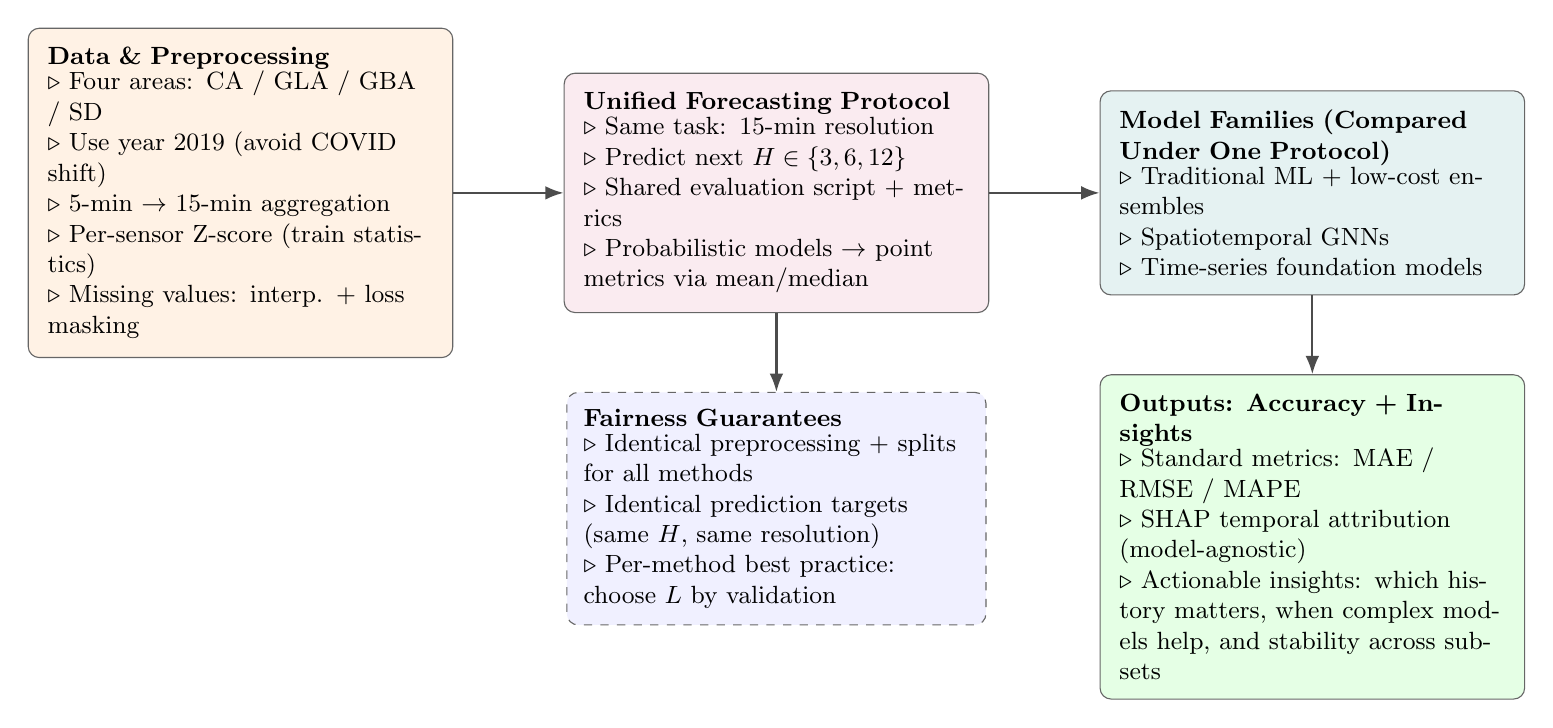
\begin{tikzpicture}[
  font=\small,
  node distance=10mm and 14mm,
  block/.style={
    draw=black!60, rounded corners, align=left,
    inner sep=7pt, text width=4.9cm, fill=gray!6
  },
  sub/.style={
    draw=black!60, rounded corners, dashed, align=left,
    inner sep=6pt, text width=4.9cm, fill=blue!6
  },
  arrow/.style={-Latex, thick, draw=black!70}
]

% ---- Column 1: Data ----
\node[block, fill=orange!10] (data) {
  \textbf{Data \& Preprocessing}\\[-2pt]
  $\triangleright$ Four areas: CA / GLA / GBA / SD\\
  $\triangleright$ Use year 2019 (avoid COVID shift)\\
  $\triangleright$ 5-min $\rightarrow$ 15-min aggregation\\
  $\triangleright$ Per-sensor Z-score (train statistics)\\
  $\triangleright$ Missing values: interp. + loss masking %\\
  %$\triangleright$ Sliding windows, stride = 1
};

% ---- Column 2: Protocol ----
\node[block, fill=purple!8, right=of data] (protocol) {
  \textbf{Unified Forecasting Protocol}\\[-2pt]
  $\triangleright$ Same task: 15-min resolution\\
  $\triangleright$ Predict next $H \in \{3,6,12\}$\\
  %$\triangleright$ Candidate contexts $L \in \{48,96,192,336,720\}$\\
  %$\triangleright$ Chronological train/val/test splits\\
  $\triangleright$ Shared evaluation script + metrics \\
  $\triangleright$ Probabilistic models $\rightarrow$ point metrics via mean/median
};

\node[sub, below=of protocol] (fairness) {
  \textbf{Fairness Guarantees}\\[-2pt]
  $\triangleright$ Identical preprocessing + splits for all methods\\
  $\triangleright$ Identical prediction targets (same $H$, same resolution)\\
  $\triangleright$ Per-method best practice: choose $L$ by validation %\\
  
};

% ---- Column 3: Models & Outputs ----
\node[block, fill=teal!10, right=of protocol] (models) {
  \textbf{Model Families (Compared Under One Protocol)}\\[-2pt]
  $\triangleright$ Traditional ML + low-cost ensembles\\
  $\triangleright$ Spatiotemporal GNNs\\
  $\triangleright$ Time-series foundation models
};

\node[block, fill=green!10, below=of models] (outputs) {
  \textbf{Outputs: Accuracy + Insights}\\[-2pt]
  $\triangleright$ Standard metrics: MAE / RMSE / MAPE\\
  %$\triangleright$ Robust baselines (e.g., mean ensembles)\\
  $\triangleright$ SHAP temporal attribution (model-agnostic)\\
  $\triangleright$ Actionable insights: which history matters, when complex models help, and stability across subsets
};

% ---- Arrows ----
\draw[arrow] (data) -- (protocol);
\draw[arrow] (protocol) -- (models);
\draw[arrow] (models) -- (outputs);
\draw[arrow] (protocol) -- (fairness);

\end{tikzpicture}%
}
\caption{Overview of the proposed unified traffic-forecasting benchmark: standardized data processing and chronological splits, a shared forecasting specification, per-method validation-based context selection to avoid unfairly constraining receptive fields, and interpretability (SHAP) to produce actionable insights beyond error metrics.}
\label{fig:benchmark_overview}
\end{figure*}



% \section{Dataset and Tasks}
% \label{sec:data}

% \textit{LargeST subsets}
% LargeST is a large-scale traffic forecasting benchmark sourced from CalTrans PeMS mainline loop
% detectors in California \citep{liu2023largest}. It provides four real-world subsets with increasing spatial
% scale: {CA} (state-wide California; 8,600 sensors), {GLA} (Greater Los Angeles; five counties; 3,834 sensors),
% {GBA} (Greater Bay Area; eleven counties; 2,352 sensors), and {SD} (San Diego county; 716 sensors). Each sensor is
% accompanied by metadata such as geographic coordinates, district, highway, travel direction, and number
% of lanes.
% The original LargeST release provides 5-minute readings from 2017--2021. Following
% the standard experimental setup used in LargeST, we aggregate 5-minute readings into {15-minute}
% windows (96 steps/day) and use {the year 2019} to reduce COVID-era distribution shift and to make
% slower baselines feasible. 


% \textit{Data prepare.}
% We aggregate 5-minute readings into non-overlapping 15-minute windows. Unless stated otherwise, the
% target is traffic \emph{flow}. We apply per-sensor $z$-score normalization using statistics computed \emph{only on the training split}.
% The same training statistics are applied to validation and test, preventing information leakage across
% time. We generate supervised instances using a stride-$H$ sliding window over time. For each $(L,H)$, an input
% consists of the most recent $L$ steps and the target consists of the next $H$ steps.




% \textit{Operational interpretation.}
% At 15-minute resolution, horizons $H=3/6/12$ correspond to 45 minutes / 1.5 hours / 3 hours
% ahead. Rather than fixing a single context length across all models, we follow each method's recommended best-practice configuration and select the input length that yields its best validation performance if accessible. This avoids penalizing methods whose design assumes a particular receptive field, while keeping the prediction targets identical across approaches. For methods that naturally output probabilistic forecasts, we compute deterministic metrics using the predictive mean. We use time-based splits, training on the first 60\% of the data points if needed, and fix the sliding window size for a fairness and best-practice configuration.


% \textit{Forecasting task}
% We study multi-step traffic flow forecasting on a directed sensor graph. Let
% $X \in \mathbb{R}^{T \times N \times C}$ denote traffic measurements over time ($T$), sensors ($N$), and
% channels ($C$). In our benchmark, we forecast {traffic flow} (typically $C=1$).
% Given a context window of length $L$,
% $\mathcal{X}_{t} = X_{t-L+1:t}$, the model predicts the next $H \in \{3, 6, 12\}$ steps:
% $\hat{X}_{t+1:t+H} = f(\mathcal{X}_{t})$.


% \textit{Interpretability and actionable insights}
% \label{sec:insights}
% Beyond accuracy, we characterize \emph{how} different model families use historical context via
% model-agnostic temporal attribution (SHAP) \citep{lundberg2017shap}. We compute attributions on the same
% deterministic quantity used for evaluation (predictive mean/median for probabilistic models) and
% aggregate attributions across sensors and time. This yields concise summaries of which lags (e.g., recent
% history vs.\ periodic components) dominate predictions under different horizons and subsets, enabling
% insights directly relevant to deployment and monitoring.


% -------------------------
% -------------------------
% \section{Models and Baselines}
% \label{sec:models}

% % --- Local definitions (safe even if defined elsewhere) ---
% \providecommand{\freq}{15\text{ min}}
% \providecommand{\ctxset}{\{48, 98, 196, 336, 720\}}
% \providecommand{\hzset}{\{3, 6, 12, 48\}}


\section{Benchmark Setup}
\label{sec:setup}

\subsection{Data, Tasks, and Diagnostic Analysis}
We evaluate on {LargeST} (Caltrans PeMS loop detectors) \citep{liu2023largest} with four subsets of increasing
scale: CA (8,600 sensors), GLA (3,834), GBA (2,352), and SD (716). Following the setup of \citet{liu2023largest},
we aggregate 5-minute readings to 15-minute resolution and use year 2019. We do not introduce new sensor measurements; our contribution is a controlled benchmark setup and
diagnostic analysis that enable reproducible, fair comparison of modern forecasting paradigms under realistic
traffic regimes.
We study multi-step traffic flow forecasting: given the most recent $L$ steps, predict the next
$H \in \{3,6,12\}$ steps (45 min / 1.5 h / 3 h). 
%All methods share the same preprocessing, chronological 60/20/20
%splits, and evaluation script. 
Rather than fixing one context length, we select each method's best-practice
context $L$ by validation from a common candidate set, keeping prediction targets identical. For probabilistic
forecasters, point metrics use the predictive mean. 

In addition, we use SHAP as a model-agnostic proxy to compare temporal reliance across heterogeneous model families; our goal is
not to fully explain each architecture, but to provide a consistent diagnostic lens that complements accuracy \citep{lundberg2017shap}. Beyond accuracy, we quantify how different model families use historical context via model-agnostic temporal
attribution (SHAP) \citep{lundberg2017shap}.  Attributions are computed on the evaluated point forecast and aggregated over
sensors/time. We report reliance profiles for representative methods by partitioning a fixed context $L$ (e.g., 48/96) into \textit{recent}, \textit{medium}, and
\textit{distant} segments and measuring their relative contributions across horizons.% $H\in\{3,6,12\}$.


\begin{table*}[t]
\centering
\caption{Performance Comparison of Forecasting Methods (San Diego Data). RMSE is dominated by a few extreme outliers at longer horizons.}
\label{tab:performance_comparison_san_diego}
\resizebox{\textwidth}{!}{
\begin{tabular}{c|c|c|c|c|c|c|c|c|c|c|c|c|c}
\toprule
Category & Method & H3 MAE & H3 RMSE & H3 MAPE & H6 MAE & H6 RMSE & H6 MAPE & H12 MAE & H12 RMSE & H12 MAPE & Avg MAE & Avg RMSE & Avg MAPE \\
\midrule
\multirow{2}{*}{Simple Baselines}
& HL & 33.61 & 50.97 & 20.77\% & 57.80 & 84.92 & 37.73\% & 101.74 & 140.14 & 76.84\% & 60.79 & 87.40 & 41.88\% \\
& Naive & 23.65 & 33.66 & 10.83\% & 35.94 & 52.99 & 24.00\% & 52.32 & 76.83 & 38.26\% & 37.30 & 54.49 & 24.36\% \\
& Seasonal Naive & 35.76 & 54.67 & 27.60\% & 29.33 & 47.65 & 23.32\% & 45.24 & 74.59 & 26.21\% & 36.78 & 58.97 & 25.71\% \\
\midrule
\multirow{4}{*}{ML Baselines}

& Ridge & 20.51 & 30.52 & 9.62\% & 27.94 & 48.86 & 23.79\% & 38.24 & 70.88 & 37.32\% & 28.90 & 50.09 & 23.58\% \\
& Random Forest & 20.05 & 30.21 & 8.42\% & 28.07 & 44.14 & 17.44\% & 35.36 & 56.02 & 20.69\% & 27.83 & 43.46 & 15.52\% \\
& Linear Regression & 20.51 & 30.52 & 9.62\% & 33.24 & - & 28.96\% & 59.47 & - & 42.89\% & 37.74 & - & 27.16\% \\
& LightGBM & 23.51 & 34.44 & 10.67\% & 30.09 & 44.59 & 23.10\% & 38.60 & 57.00 & 30.59\% & 30.73 & 45.34 & 21.45\% \\
\midrule
\multirow{3}{*}{Ensembles}
& Median & 19.18 & 28.71 & 8.76\% & 24.30 & 39.29 & 18.75\% & 32.41 & 53.03 & 27.22\% & 25.30 & 40.34 & 18.24\% \\
& Mean & 19.61 & 29.13 & 11.89\% & 23.90 & - & 20.01\% & 36.65 & - & 27.76\% & 26.72 & - & 19.89\% \\
& Weighted & 19.26 & 28.57 & 10.46\% & 24.68 & - & 19.84\% & 35.78 & - & 27.48\% & 26.57 & - & 19.26\% \\
\midrule
\multirow{10}{*}{GNN-based}
& AGCRN & 15.71 & 27.85 & 11.48\% & 18.06 & 31.51 & 13.06\% & 21.86 & 39.44 & 16.52\% & 18.09 & 32.01 & 13.28\% \\
& ASTGCN & 19.56 & 31.33 & 12.18\% & 24.13 & 37.95 & 15.38\% & 30.96 & 49.17 & 21.98\% & 23.70 & 37.63 & 15.65\% \\
& D2STGNN & \textbf{14.92} & 24.95 & 9.56\% & 17.52 & 29.24 & 11.36\% & 22.62 & 37.14 & 14.86\% & 17.85 & 29.51 & 11.54\% \\
& DCRNN & 17.14 & 27.47 & 11.12\% & 20.99 & 33.29 & 13.95\% & 26.99 & 42.86 & 18.67\% & 21.03 & 33.37 & 14.13\% \\
& DGCRN & 15.34 & 25.35 & 10.01\% & 18.05 & 30.06 & 11.90\% & 22.06 & 37.51 & 15.27\% & 18.02 & 30.09 & 12.07\% \\
& DSTAGNN & 18.13 & 28.96 & 11.38\% & 21.71 & 34.44 & 13.93\% & 27.51 & 43.95 & 19.34\% & 21.82 & 34.68 & 14.40\% \\
& GWNET & \underline{15.24} & 25.13 & 9.86\% & 17.74 & 29.51 & 11.70\% & 21.56 & 36.82 & 15.13\% & 17.74 & 29.62 & 11.88\% \\
& STGCN & 17.45 & 29.99 & 12.42\% & 19.55 & 33.69 & 13.68\% & 23.21 & 41.23 & 16.32\% & 19.67 & 34.14 & 13.86\% \\
& STGODE & 16.75 & 28.04 & 11.00\% & 19.71 & 33.56 & 13.16\% & 23.67 & 42.12 & 16.58\% & 19.55 & 33.57 & 13.22\% \\
& STTN & 16.22 & 26.22 & 10.63\% & 18.76 & 30.98 & 12.80\% & 22.62 & 39.09 & 16.14\% & 18.69 & 31.11 & 12.82\% \\
\midrule
\multirow{1}{*}{RNN-based}
& LSTM & 19.03 & 30.53 & 11.81\% & 25.84 & 40.87 & 16.44\% & 37.63 & 59.07 & 25.45\% & 26.44 & 41.73 & 17.20\% \\
\midrule
\multirow{8}{*}{Foundation Models}
& FlowState & 17.10 & 25.90 & 7.26\% & 16.60 & 26.50 & 10.09\% & 17.90 & 28.74 & 10.14\% & 17.20 & 27.05 & 9.16\% \\
& Chronos-2 & 16.15 & \textbf{24.70} & \underline{6.83\%} & 15.48 & \textbf{24.89} & 9.21\% & \textbf{16.42} & \textbf{27.01} & \textbf{9.43\%} & \underline{16.02} & \textbf{25.53} & \underline{8.49\%} \\
& Chronos-Bolt & 17.24 & 26.36 & 7.12\% & 16.46 & 26.50 & 9.60\% & 17.47 & 28.20 & 9.97\% & 17.06 & 27.02 & 8.90\% \\
& Kairos & 17.70 & 26.50 & 7.49\% & 17.81 & 28.49 & 10.97\% & 19.23 & 30.25 & 11.63\% & 18.25 & 28.41 & 10.03\% \\
& Moirai-2 & 16.57 & 25.27 & 6.94\% & 16.41 & 27.71 & 9.64\% & 17.59 & 29.83 & 10.03\% & 16.86 & 27.60 & 8.87\% \\
& Moirai-Small & 24.44 & - & 10.10\% & 28.88 & - & 19.90\% & 36.70 & - & 24.51\% & 30.01 & - & 18.17\% \\
& TimesFM & 19.35 & 28.29 & 7.98\% & 20.75 & 32.45 & 12.10\% & 21.37 & 33.54 & 12.29\% & 20.49 & 31.43 & 10.79\% \\
& Sundial & 15.79 & \underline{24.87} & \textbf{6.62\%} & \textbf{15.12} & \underline{25.10} & \textbf{9.01\%} & \underline{16.78} & \underline{27.50} & \underline{9.62\%} & \textbf{15.90} & \underline{25.82} & \textbf{8.42\%} \\
\bottomrule
\end{tabular}
}

\end{table*}


% -------------------------
\subsection{Models and Baselines}
\label{sec:models}

We benchmark forecasting methods spanning: (i) simple rule-based baselines, (ii) classical ML regressors,
(iii) low-cost ensembles, (iv) spatiotemporal GNN architectures tailored to traffic networks, (v) an RNN
sequence baseline, and (vi) pretrained time-series foundation models.

\subsubsection{Simple baselines}

We include transparent baselines as sanity checks for short-horizon traffic forecasting \citep{hyndman2021fpp}.

\textit{HL:}
A historical-level baseline that predicts using a simple persistence/level heuristic (as implemented in our codebase).

\textit{Naive:}
A persistence baseline that repeats the most recent observation \citep{hyndman2021fpp}.

\textit{Seasonal Naive:}
A seasonal persistence baseline that repeats the value from the same time-of-day in the previous cycle
(e.g., same 15-minute slot one day ago) \citep{hyndman2021fpp}.

\subsubsection{Machine Learning Methods}
Classical ML baselines recast forecasting as supervised regression on lag features. For each sensor,
we form a feature vector from the past $L$ observations and train a regressor to predict the next step;
multi-step forecasts up to horizon $H$ are produced via iterative roll-out.

\textit{Linear regression:}
Ordinary least squares on lag features (a minimal linear baseline).

\textit{Ridge regression:}
Linear regression with $\ell_2$ regularization to stabilize estimation under correlated lag features \citep{hoerl1970ridge}.

\textit{Random Forest:}
A bagged ensemble of decision trees to capture non-linear interactions among lags \citep{breiman2001randomforest}.

\textit{LightGBM:}
Gradient-boosted decision trees with efficient histogram-based training and strong tabular performance \citep{ke2017lightgbm}.

\textit{Ensemble models:}
Ensembles improve robustness by combining heterogeneous predictors \citep{bates1969combination}.
Let $\{\hat{\mathbf{x}}^{(k)}\}_{k=1}^K$ be the $H$-step forecasts from $K$ base models (here, combinations of
SeasonalNaive/ Ridge/ LinearRegression/ RandomForest as instantiated by our ensemble variants). We use a weighted ensemble:
\begin{equation}
\hat{\mathbf{x}}^{\text{ens}}=\sum_{k=1}^K w_k \hat{\mathbf{x}}^{(k)}, \qquad
\sum_{k=1}^K w_k=1,\;\; w_k\ge 0,
\end{equation}
with weights selected on the validation set. The mean ensemble is the special case $w_k = 1/K$,
and the median ensemble uses the coordinate-wise median across $\{\hat{\mathbf{x}}^{(k)}\}$.

\subsubsection{Task-Trained Deep Learning  Models}


\textit{GNN-based models:}
Spatiotemporal GNNs forecast jointly across sensors by combining temporal modeling with graph-based spatial
message passing, matching the inductive structure of traffic networks. We include widely used architectures:
DCRNN \citep{li2018dcrnn}, STGCN \citep{yu2018stgcn}, Graph WaveNet (GWNET) \citep{wu2019graphwavenet},
ASTGCN \citep{guo2019attention}, and AGCRN \citep{bai2020adaptive}, plus additional traffic GNN variants
(DGCRN~\citep{li2021dynamic}, STGODE~\citep{fang2021spatial}, STTN~\citep{xu2020spatial}, DSTAGNN~\citep{lan2022dstagnn}, D2STGNN~\citep{shao2022decoupled}) following prior benchmarking practice \citep{liu2023needgnn, lan2022dstagnn}.

\textit{LSTM:}
We include an LSTM forecaster as a canonical sequence model baseline \citep{hochreiter1997lstm}.

\subsubsection{Foundation Models}
Time-series foundation models are pretrained on large and diverse corpora and can be applied to new domains
in (primarily) zero-shot mode. We evaluate Chronos-2 \citep{ansari2024chronos} (and a Chronos-Bolt variant built
on the Chronos family), Moirai-2 and Moirai-Small \citep{woo2024moirai},
TimesFM \citep{das2024timesfm}, Kairos \citep{feng2025kairos}, Sundial (sundial\_base\_128m) \citep{liu2025sundial},
and FlowState-9.1M \citep{graf2025flowstate}. For probabilistic models, we compute point metrics using the predictive mean.
%(or median when more appropriate).

%\subsection{SHAP value via temporal attribution}



%\textit{Operational Observations.} Our analysis reveals distinct patterns in information utilization.  Foundation models tend to allocate a higher proportion of importance to \textit{remote} history, suggesting they successfully extract long-range temporal dependencies.  In contrast, linear models often distribute importance more uniformly or focus heavily on the most recent observations, particularly in short-horizon scenarios ($H=3$).  These profiles provide critical insights for practitioners regarding model stability and robustness under distribution shifts. 

% -------------------------
% \section{Experimental Protocol}
% \label{sec:protocol}

% \subsection{Unified preprocessing}
% We standardize:
% \begin{itemize}[leftmargin=1.2em]
%   \item time alignment and \freq{} resampling,
%   \item missing-value handling and masking,
%   \item normalization/scaling (applied consistently across model families),
%   \item context/horizon windowing and dataset serialization.
% \end{itemize}
% \TODO{Specify the exact preprocessing steps used in the repo (e.g., z-score per sensor, global scaling, interpolation strategy).}

% \subsection{Training configuration}
% \begin{itemize}[leftmargin=1.2em]
%   \item Hardware: \TODO{GPU/CPU/RAM}.
%   \item Training length: \TODO{epochs} epochs; early stopping on validation.
%   \item Optimizer + LR: \TODO{Adam/SGD, learning rate schedule}.
%   \item Batch size: \TODO{...}.
% \end{itemize}

% \subsection{Code entry points}
% We provide standardized entry points:
% \begin{itemize}[leftmargin=1.2em]
%   \item \texttt{benchmark/}: unified evaluation utilities and metrics,
%   \item \texttt{experiments/}: training runs (ML/GNN/foundation),
%   \item \texttt{gift-eval/}: evaluation helper scripts (if applicable),
%   \item \texttt{interpret/}: SHAP pipeline and plotting.
% \end{itemize}
% \TODO{Replace with the exact script/module names from your repo.}

% \subsection{Seeds and repeatability}
% We fix random seeds and report mean $\pm$ std for stochastic methods (e.g., GNN training).
% \TODO{State number of repeats, seed list, and how results are aggregated.}










\begin{table*}[t]
\centering
\caption{Performance Comparison of Forecasting Methods (Bay Area Data)}
\label{tab:performance_comparison_bay_area}
\resizebox{\textwidth}{!}{
\begin{tabular}{c|c|c|c|c|c|c|c|c|c|c|c|c|c}
\toprule
Category & Method & H3 MAE & H3 RMSE & H3 MAPE & H6 MAE & H6 RMSE & H6 MAPE & H12 MAE & H12 RMSE & H12 MAPE & Avg MAE & Avg RMSE & Avg MAPE \\
\midrule
\multirow{3}{*}{Simple Baselines} & HL & 32.57 & 48.42 & 22.78\% & 53.79 & 77.08 & 43.01\% & 92.64 & 126.22 & 92.85\% & 56.44 & 79.82 & 48.87\% \\
& Naive & 22.34 & 33.42 & 11.00\% & 33.63 & 48.75 & 26.48\% & 50.99 & 75.10 & 45.46\% & 35.65 & 52.42 & 27.64\% \\
& Seasonal Naive & 39.17 & 62.10 & 16.12\% & 34.89 & 56.73 & 18.62\% & 49.37 & 76.59 & 28.15\% & 41.14 & 65.14 & 20.96\% \\
\midrule
\multirow{4}{*}{ML Baselines} 
& Ridge & 19.24 & 30.18 & 9.37\% & 26.23 & 38.60 & 26.93\% & 38.78 & 60.01 & 45.68\% & 28.08 & 42.93 & 27.33\% \\
& Random Forest & 22.12 & 33.66 & 9.39\% & 27.49 & 42.40 & 19.18\% & 35.06 & 54.19 & 23.73\% & 28.22 & 43.42 & 17.43\% \\
& Linear Regression & 19.24 & 30.18 & 9.37\% & 26.95 & - & 28.30\% & 38.79 & 60.16 & 45.71\% & 28.33 & - & 27.76\% \\
& LightGBM & 23.10 & 34.32 & 10.56\% & 28.99 & 42.01 & 27.69\% & 37.89 & 55.47 & 36.41\% & 29.99 & 43.94 & 24.88\% \\

\midrule
\multirow{3}{*}{Ensembles} & Median & 18.51 & 29.29 & 8.60\% & 23.20 & 34.87 & 20.93\% & 33.67 & 50.32 & 33.82\% & 25.13 & 38.16 & 21.12\% \\
& Mean & 19.50 & 30.34 & 8.81\% & 22.04 & - & 19.42\% & 32.44 & 48.26 & 31.62\% & 24.66 & - & 19.95\% \\
& Weighted & 18.81 & 29.35 & 8.56\% & 22.73 & 73.90 & 20.23\% & 32.24 & 48.13 & 31.76\% & 24.59 & 50.46 & 20.18\% \\

\midrule
\multirow{10}{*}{GNN-based} & AGCRN & 18.31 & 30.24 & 14.27\% & 21.27 & 34.72 & 16.89\% & 24.85 & 40.18 & 20.80\% & 21.01 & 34.25 & 16.90\% \\
& ASTGCN & 21.46 & 33.86 & 17.24\% & 26.96 & 41.38 & 24.22\% & 34.29 & 52.44 & 32.53\% & 26.47 & 40.99 & 23.65\% \\
& D2STGNN & 17.54 & 28.94 & 12.12\% & 20.92 & 33.92 & 14.89\% & 25.48 & 40.99 & 19.83\% & 20.71 & 33.65 & 15.04\% \\
& DCRNN & 18.71 & 30.36 & 14.72\% & 23.06 & 36.16 & 20.45\% & 29.85 & 46.06 & 29.93\% & 23.13 & 36.35 & 20.84\% \\
& DGCRN & 18.02 & 29.49 & 14.13\% & 21.08 & 34.03 & 16.94\% & 25.25 & 40.63 & 21.15\% & 20.91 & 33.83 & 16.88\% \\
& DSTAGNN & 19.73 & 31.39 & 15.42\% & 24.21 & 37.70 & 20.99\% & 30.12 & 46.40 & 28.16\% & 23.82 & 37.29 & 20.16\% \\
& GWNET & 17.85 & 29.12 & 13.92\% & 21.11 & 33.69 & 17.79\% & 25.58 & 40.19 & 23.48\% & 20.91 & 33.41 & 17.66\% \\
& STGCN & 21.05 & 34.51 & 16.42\% & 23.63 & 38.92 & 18.35\% & 26.87 & 44.45 & 21.92\% & 23.42 & 38.57 & 18.46\% \\
& STGODE & 18.84 & 30.51 & 15.43\% & 22.04 & 35.61 & 18.42\% & 26.22 & 42.90 & 22.83\% & 21.79 & 35.37 & 18.26\% \\
& STTN & 18.25 & 29.64 & 14.05\% & 21.06 & 33.87 & 17.03\% & 25.29 & 40.58 & 21.20\% & 20.97 & 33.78 & 16.84\% \\

\midrule
\multirow{1}{*}{RNN-based} & LSTM & 20.38 & 33.34 & 15.47\% & 27.56 & 43.57 & 23.52\% & 39.03 & 60.59 & 37.48\% & 27.96 & 44.21 & 24.48\% \\

\midrule
\multirow{8}{*}{Foundation Models} & FlowState& 15.72 & 26.76 & 6.72\% & 16.13 & 27.20 & 11.08\% & 19.83 & 32.53 & 13.49\% & 17.23 & 28.83 & 10.43\% \\
& Chronos-2 & \textbf{13.92} & \textbf{25.01} & \textbf{5.63\%} & \textbf{14.39} & \textbf{25.12} & \textbf{9.67\%} & \textbf{17.61} & \textbf{30.13} & \textbf{11.52\%} & \textbf{15.31} & \textbf{26.75} & \textbf{8.94\%} \\
& Chronos-Bolt & 15.06 & 25.92 & 6.32\% & 15.76 & 26.21 & 10.68\% & 19.45 & 31.69 & 12.99\% & 16.76 & 27.94 & 10.00\% \\
& Kairos & 14.92 & \underline{25.51} & 6.27\% & 15.78 & 26.11 & 10.64\% & 19.88 & 31.54 & 13.60\% & 16.86 & 27.72 & 10.17\% \\
& Moirai-Small & 25.61 & 37.78 & 12.79\% & 31.31 & 45.73 & 25.81\% & 39.50 & 58.97 & 33.61\% & 32.14 & 47.49 & 24.07\% \\
& Moirai-2 & 14.90 & 25.84 & 6.25\% & 15.77 & 26.59 & 10.63\% & 19.27 & 31.49 & 13.17\% & 16.64 & 27.97 & 10.02\% \\
& TimesFM & 16.28 & 27.53 & 6.74\% & 18.06 & 30.25 & 12.24\% & 21.47 & 35.18 & 14.49\% & 18.60 & 30.99 & 11.15\% \\
& Sundial& \underline{14.38} & 25.63 & \underline{5.94\%} & \underline{15.09} & \underline{25.94} & 10.28\% & \underline{19.00} & \underline{31.32} & 12.88\% & \underline{16.15} & \underline{27.63} & \underline{9.70\%} \\

\bottomrule
\end{tabular}
}

\end{table*}

\begin{table*}[t]
\centering
\caption{Performance Comparison of Forecasting Methods (CA Data)}
\label{tab:performance_comparison_ca}
\resizebox{\textwidth}{!}{
\begin{tabular}{c|c|c|c|c|c|c|c|c|c|c|c|c|c}
\toprule
Category & Method & H3 MAE & H3 RMSE & H3 MAPE & H6 MAE & H6 RMSE & H6 MAPE & H12 MAE & H12 RMSE & H12 MAPE & Avg MAE & Avg RMSE & Avg MAPE \\

\midrule
\multirow{2}{*}{Simple Baselines}
& HL
& 30.72 & 46.96 & 20.43\% 
& 51.56 & 76.48 & 37.22\% 
& 89.31 & 125.71 & 76.80\% 
& 57.20 & 83.05 & 44.82\% \\

& Naive
& 21.22 & 32.55 & 11.10\% 
& 32.66 & 49.17 & 24.14\% 
& 48.17 & 73.35 & 39.37\% 
& 34.02 & 51.69 & 24.87\% \\
& Seasonal Naive
& 34.39 & 57.65 & 19.37\% 
& 30.64 & 52.10 & 20.33\% 
& 43.86 & 72.13 & 26.64\% 
& 36.29 & 60.63 & 22.11\% \\

\midrule
\multirow{5}{*}{ML Baselines}


& Ridge
& 18.74 & 29.78 & 10.07\% 
& 25.83 & 40.07 & 24.87\% 
& 36.66 & 73.52 & 39.70\% 
& 27.08 & 47.79 & 24.88\% \\

& Random Forest
& 17.26 & 29.49 & 8.11\% 
& 20.69 & 35.60 & 13.04\% 
& 26.99 & 46.11 & 17.52\% 
& 21.65 & 37.07 & 12.89\% \\

& Linear Regression
& 18.74 & 29.78 & 10.07\% 
& 85.87 & - & 45.43\% 
& 38.45 & - & 40.18\% 
& 47.69 & - & 31.89\% \\

& LightGBM
& 21.64 & 33.08 & 11.19\% 
& 27.40 & 40.79 & 24.13\% 
& 35.43 & 53.34 & 32.27\% 
& 28.16 & 42.41 & 22.53\% \\

\midrule
\multirow{3}{*}{Ensembles}
& Median
& 17.65 & 28.38 & 9.22\% 
& 22.43 & 34.65 & 19.53\% 
& 31.09 & 53.03 & 29.71\% 
& 23.72 & 38.69 & 19.49\% \\

& Mean
& 18.26 & 28.78 & 10.20\% 
& 36.21 & - & 23.63\% 
& 30.68 & - & 28.49\% 
& 28.38 & - & 20.77\% \\

& weighted
& 17.82 & 28.12 & 9.67\% 
& 33.91 & - & 23.07\% 
& 30.47 & - & 28.62\% 
& 27.40 & - & 20.45\% \\
\midrule

\multirow{10}{*}{GNN-based}
& AGCRN
& 15.71 & 27.85 & 11.48\% 
& 18.06 & 31.51 & 13.06\% 
& 21.86 & 39.44 & 16.52\% 
& 18.54 & 32.93 & 13.69\% \\

& ASTGCN
& 19.56 & 31.33 & 12.18\% 
& 24.13 & 37.95 & 15.38\% 
& 30.96 & 49.17 & 21.98\% 
& 24.88 & 39.48 & 16.51\% \\

& D2STGNN
& 14.92 & 24.95 & 9.56\% 
& 17.52 & 29.24 & 11.36\% 
& 22.62 & 37.14 & 14.86\% 
& 18.35 & 30.44 & 11.93\% \\

& DCRNN
& 17.14 & 27.47 & 11.12\% 
& 20.99 & 33.29 & 13.95\% 
& 26.99 & 42.86 & 18.67\% 
& 21.71 & 34.54 & 14.58\% \\

& DGCRN
& 15.34 & 25.35 & 10.01\% 
& 18.05 & 30.06 & 11.90\% 
& 22.06 & 37.51 & 15.27\% 
& 18.48 & 30.97 & 12.39\% \\

& DSTAGNN
& 18.13 & 28.96 & 11.38\% 
& 21.71 & 34.44 & 13.93\% 
& 27.51 & 43.95 & 19.34\% 
& 22.45 & 35.78 & 14.88\% \\

& GWNET
& 15.24 & 25.13 & 9.86\% 
& 17.74 & 29.51 & 11.70\% 
& 21.56 & 36.82 & 15.13\% 
& 18.18 & 30.49 & 12.23\% \\

& STGCN
& 17.45 & 29.99 & 12.42\% 
& 19.55 & 33.69 & 13.68\% 
& 23.21 & 41.23 & 16.32\% 
& 20.07 & 34.97 & 14.14\% \\

& STGODE
& 16.75 & 28.04 & 11.00\% 
& 19.71 & 33.56 & 13.16\% 
& 23.67 & 42.12 & 16.58\% 
& 20.04 & 34.57 & 13.58\% \\

& STTN
& 16.22 & 26.22 & 10.63\% 
& 18.76 & 30.98 & 12.80\% 
& 22.62 & 39.09 & 16.14\% 
& 19.20 & 32.10 & 13.19\% \\

\midrule
\multirow{8}{*}{Foundation Models}
& FlowState
& 15.02 & 26.16 & 7.36\% 
& 15.08 & 25.64 & 10.45\% 
& 17.39 & 29.15 & 11.64\% 
& 15.83 & 26.98 & 9.82\% \\

& Chronos-2
& \textbf{13.57} & \textbf{24.27} & \textbf{6.44\%} 
& \textbf{13.57} & \textbf{23.85} & \textbf{9.38\%} 
& \textbf{15.62} & \textbf{27.63} & \textbf{10.32\%} 
& \textbf{14.25} & \textbf{25.25} & \textbf{8.71\%} \\

& Chronos-Bolt
& 14.84 & 25.59 & 7.12\% 
& 15.12 & 25.38 & 10.21\% 
& 17.48 & 29.12 & 11.36\% 
& 15.81 & 26.70 & 9.56\% \\

& Kairos
& 14.74 & 25.26 & 7.05\% 
& 15.31 & 25.73 & 10.33\% 
& 17.95 & 29.60 & 12.04\% 
& 15.99 & 26.86 & 9.81\% \\

& Moirai-2
& 14.30 & 25.25 & 6.84\% 
& 14.84 & 25.61 & 9.90\% 
& 17.23 & 29.39 & 11.33\% 
& 15.46 & 26.75 & 9.36\% \\

& Moirai-Small
& 24.65 & 42.57 & 13.27\% 
& 30.97 & 50.68 & 24.06\% 
& 37.40 & 69.22 & 30.07\% 
& 31.01 & 54.16 & 22.47\% \\

& TimesFM 
& 15.78 & 26.58 & 7.39\% 
& 17.12 & 28.87 & 11.45\% 
& 19.15 & 32.11 & 12.67\% 
& 17.35 & 29.19 & 10.50\% \\

& Sundial
& \underline{13.85} & \underline{24.74} & \underline{6.61\%} 
& \underline{14.10} & \underline{24.57} & \underline{9.62\%} 
& \underline{16.81} & \underline{28.81} & \underline{11.19\%} 
& \underline{14.92} & \underline{26.04} & \underline{9.14\%} \\

\bottomrule
\end{tabular}
}
\end{table*}




\section{Experimental Results}
\label{sec:results}

\textit{Experimental coverage and space constraints.}
Due to limited space, we report the full set of results for CA/GBA/SD in the main paper and move the complete
Greater Los Angeles (GLA) tables and analysis to the appendix. The GLA subset follows the same protocol and
evaluation pipeline; we include it as an additional large-scale urban test case to verify that the observed
trends are consistent across regions.

\subsection{San Diego (SD) Results}
\label{sec:sd_results}

% Table~\ref{tab:performance_comparison_san_diego} reports forecasting performance on the SD subset
% across horizons $H\in\{3,6,12\}$. Overall, SD exhibits a clear separation between simple heuristics, tabular ML (and their ensembles), graph-aware spatiotemporal models, and pretrained foundation models.


% Rule-based heuristics degrade rapidly as the horizon grows. HL suffers severe error accumulation
% (MAE: 33.61 $\rightarrow$ 57.80 $\rightarrow$ 101.74 from $H=3$ to $H=12$), confirming that pure
% persistence is not operationally useful beyond the shortest horizon. Naive is substantially stronger than HL but still shows pronounced degradation (Avg MAE 37.30).
% Among single ML regressors, \texttt{random\_forest} is the strongest overall (Avg MAE/RMSE/MAPE
% $=27.83/43.46/15.52\%$), outperforming ridge and lightgbm. Importantly, simple ensembles of classical
% predictors provide a consistent boost: the \texttt{median} ensemble achieves Avg MAE 25.30, improving
% over the best single ML model by $\approx 9.1\%$ (25.30 vs.\ 27.83) with essentially negligible
% engineering overhead. Notably, these low-cost ensembles are also competitive with the LSTM baseline (Avg MAE 26.44), suggesting that careful aggregation of strong tabular predictors can match or exceed
% a temporal-only neural model on SD.

% GNN-based methods substantially improve over ML baselines at short horizons. D2STGNN attains the best
% $H=3$ MAE (14.92), while GWNET provides the best average MAE among GNNs (Avg MAE 17.74), indicating robust performance from graph propagation with temporal convolution. However, compared with the foundation models, GNNs show steeper error growth with horizon (e.g., D2STGNN MAE increases by $\approx 51.6\%$ from $H=3$ to $H=12$: 14.92 $\rightarrow$ 22.62), highlighting reduced mid-horizon stability on SD.

% Pretrained foundation models are highly competitive on SD and dominate medium horizons. The best overall average accuracy (by MAE/MAPE) is achieved by \texttt{sundial\_base\_128m} (Avg MAE/MAPE $=15.90/8.42\%$), while \texttt{Chronos-2} achieves the best Avg RMSE (25.53) and the strongest $H=12$ performance (MAE/RMSE $=16.42/27.01$). Foundation models also exhibit markedly flatter horizon degradation: Chronos-2’s MAE increases by only $\approx 1.7\%$ from $H=3$ to $H=12$
% (16.15 $\rightarrow$ 16.42), compared with $>40\%$ growth for strong GNN baselines such as GWNET.
% This suggests that large-scale pretraining provides robust transfer and improved medium-range stability even without explicitly encoding the road graph.

% \textit{Takeaway:}
% On SD, spatiotemporal GNNs remain the most accurate family at the shortest horizon (e.g., D2STGNN at $H=3$),
% but foundation models provide substantially better horizon stability and the best overall averages
% (\texttt{sundial\_base\_128m} / \texttt{Chronos-2}). Meanwhile, classical ensembles offer a strong
% ``low-cost'' option that materially improves upon single ML baselines and can rival simple neural models.

Table~\ref{tab:performance_comparison_san_diego} summarizes results on SD for $H\in\{3,6,12\}$.
Simple heuristics degrade quickly with horizon: HL accumulates error severely (MAE
33.61$\rightarrow$57.80$\rightarrow$101.74), while Naive is stronger but still unstable (Avg MAE 37.30).
Among tabular ML, \texttt{random\_forest} is best (Avg MAE 27.83), and low-cost ensembles provide a reliable boost:
the \texttt{median} ensemble reaches Avg MAE 25.30, a $\approx9.1\%$ improvement over the best single ML model and
competitive with the temporal-only \texttt{LSTM} baseline (Avg MAE 26.44).

STGNNs substantially improve short-horizon accuracy. \texttt{D2STGNN} attains the best $H{=}3$ MAE (14.92), and
\texttt{GWNET} is the strongest GNN on average (Avg MAE 17.74). However, their errors grow more steeply with
horizon (e.g., \texttt{D2STGNN} MAE 14.92$\rightarrow$22.62 from $H{=}3$ to $H{=}12$), whereas pretrained
foundation models are markedly more stable and dominate mid-horizon performance. The best overall averages
(by MAE/MAPE) are achieved by \texttt{sundial\_base\_128m} (Avg MAE/MAPE $=15.90/8.42\%$), while \texttt{Chronos-2}
yields the best Avg RMSE (25.53) and the strongest $H{=}12$ results (MAE/RMSE $=16.42/27.01$). Notably,
\texttt{Chronos-2} exhibits near-flat degradation across horizons, with MAE increasing by only $\approx 1.7\%$
(16.15$\rightarrow$16.42), compared with $>40\%$ growth for strong GNN baselines such as \texttt{GWNET}. These
patterns suggest that large-scale pretraining confers robust transfer and improved medium-range stability even
without explicitly encoding the road graph.


%The best overall averages are
%obtained by \texttt{sundial\_base\_128m} (Avg MAE/MAPE 15.90/8.42\%), while \texttt{Chronos-2} yields the best Avg
%RMSE (25.53) and strongest $H{=}12$ accuracy (MAE/RMSE 16.42/27.01), with near-flat MAE growth across horizons
%(16.15$\rightarrow$16.42).
\begin{keydiscovery1}
\textit{Takeaway:} On SD, GNNs lead at the shortest horizon, but foundation models provide the best overall accuracy
and markedly better horizon stability; classical ensembles remain a strong, low-cost baseline that can rival simple
neural models.
\end{keydiscovery1}







%\TODO{Verify if cross-dataset transfer (e.g., GLA $\to$ GBA) provides foundation models with an additional performance edge compared to GNNs trained from scratch.}




\subsection{ Bay Area (GBA) Results}
\label{sec:results_bay_area}

The Greater Bay Area (GBA) subset is a challenging setting due to its large spatial extent and heterogeneous
traffic dynamics. Table~\ref{tab:performance_comparison_bay_area} summarizes results at horizons
$H\in\{3,6,12\}$. Classical ML baselines are substantially improved by ensembling: the best ensemble (\texttt{weighted}) achieves Avg MAE 24.59, outperforming single regressors (e.g., ridge 28.08, lightgbm 29.99) and the LSTM
baseline (Avg MAE 27.96). However, even these strong low-cost baselines remain far behind pretrained models. GNNs remain competitive at short horizons but lag in mid-range stability. Among GNN-based methods, \texttt{D2STGNN} is the strongest (Avg MAE 20.71), followed closely by
\texttt{DGCRN}/\texttt{GWNET}/\texttt{STTN} (Avg MAE $\approx 20.9$--21.0). While these models leverage spatial
structure effectively, their errors grow faster with horizon (e.g., D2STGNN: 17.54 $\rightarrow$ 25.48).
Notably, heavier architectures such as \texttt{ASTGCN} and \texttt{DSTAGNN} underperform relative to more
efficient designs, reinforcing that stronger inductive bias and optimization behavior matter more than raw
capacity on GBA.

Across all horizons and metrics, \texttt{Chronos-2} ranks first (Avg MAE/RMSE/MAPE $=15.31/26.75/8.94\%$),
achieving the best performance at $H=3$ (MAE 13.92), $H=6$ (MAE 14.39), and $H=12$ (MAE 17.61).
Other foundation models are consistently strong, including \texttt{sundial} (Avg MAE 16.15),
\texttt{Moirai-2} (16.64), \texttt{Chronos-Bolt} (16.76), and \texttt{Kairos} (16.86), indicating that
large-scale pretraining transfers well to GBA without explicitly encoding the road graph.
A key insight is \emph{horizon stability}: Chronos-2’s MAE increases by only $\approx 26.5\%$ from $H=3$ to
$H=12$ (13.92 $\rightarrow$ 17.61), suggesting robust medium-range extrapolation.



\begin{keydiscovery1}
\textit{Takeaway:}
On GBA, foundation models set the accuracy and robustness frontier (best overall and best stability), GNNs offer strong graph-aware short-horizon performance but weaker horizon scaling, and classical ensembles provide
a practical improvement over single ML baselines while still leaving a sizable gap to pretrained models.
\end{keydiscovery1}




\begin{figure}[t]
    \centering
    \begin{subfigure}[t]{0.48\linewidth}%
        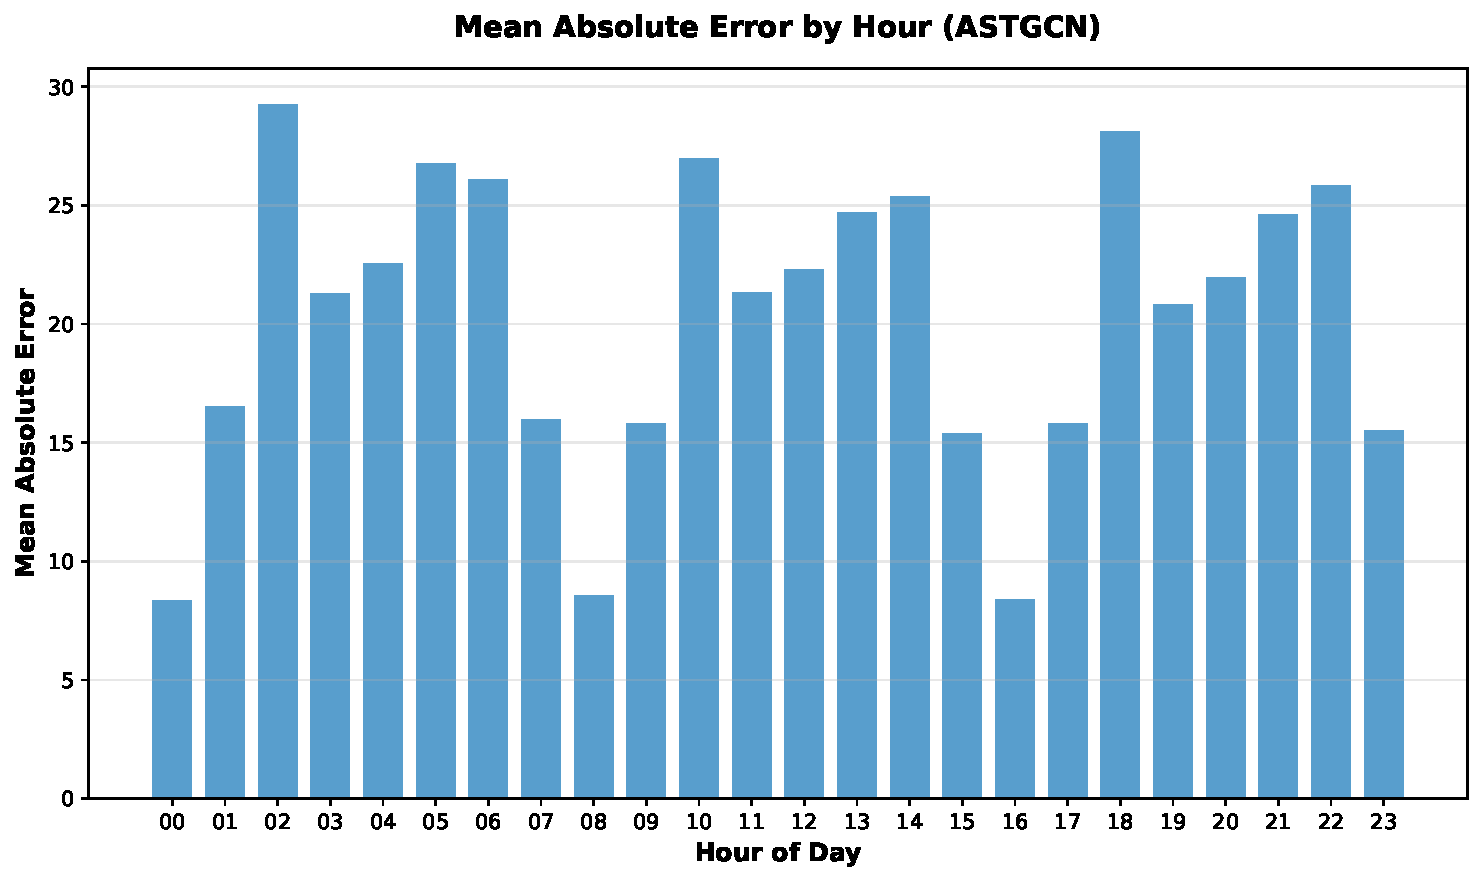
\includegraphics[width=\linewidth]{images/time_interval/ASTGCN_hourly_mean_abs_error.pdf}%
        \caption{\textbf{ASTGCN}. Errors are elevated in late-night low-demand periods (notably around 02:00) and again near the evening peak, indicating regime-dependent sensitivity that is not visible from aggregate scores alone.}%
        \label{fig:ASTGCN_hourly_mean_abs_error}%
    \end{subfigure}%
    \hfill
    \begin{subfigure}[t]{0.48\linewidth}%
        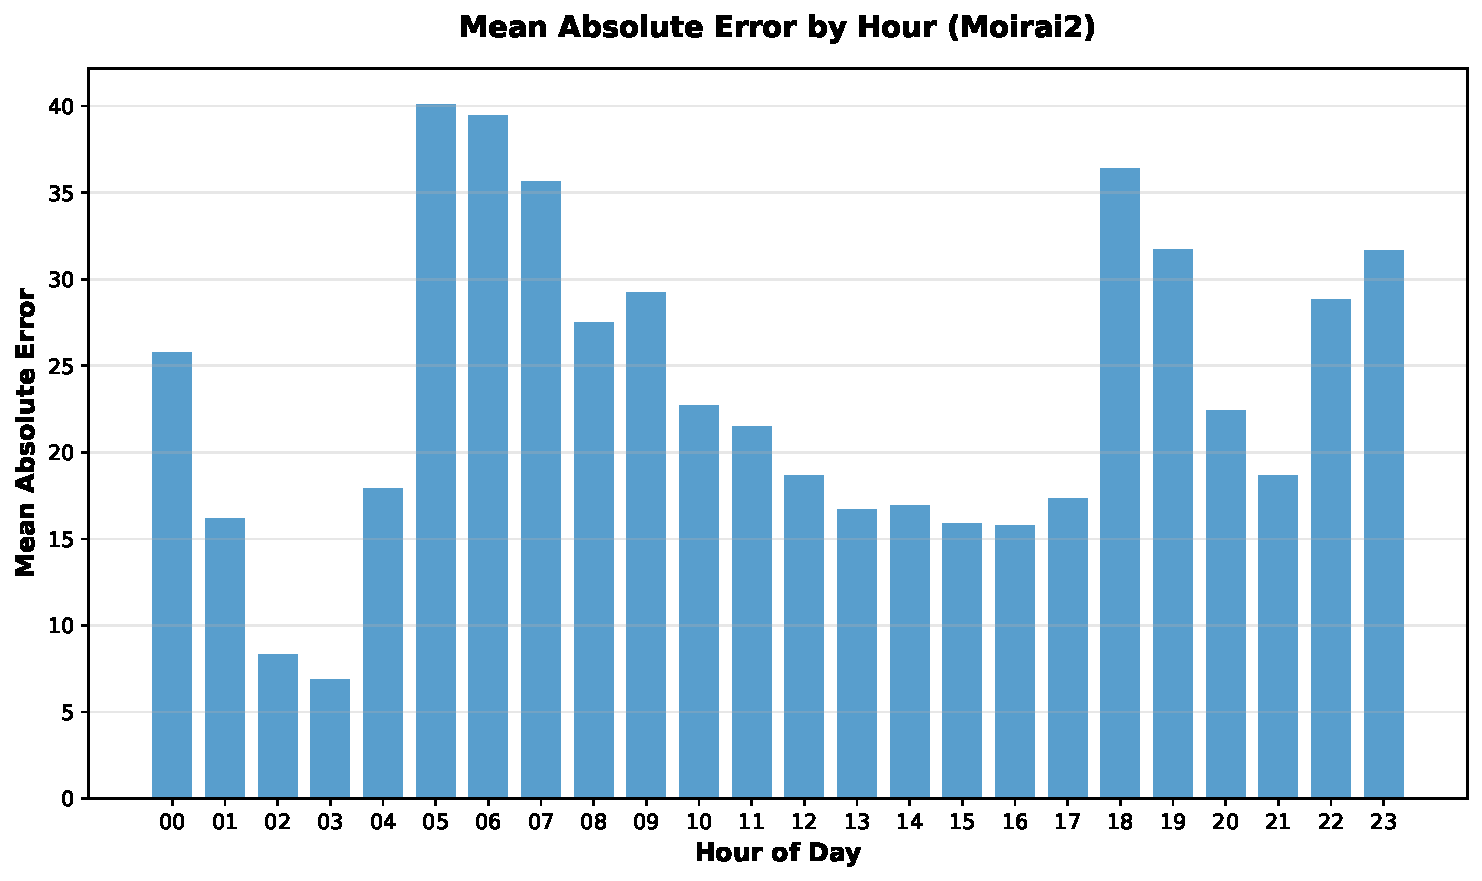
\includegraphics[width=\linewidth]{images/time_interval/Moiria2_hourly_mean_abs_error.pdf}%
        \caption{\textbf{Moirai2}. The model is relatively accurate overnight (02:00--04:00) but exhibits sharp error spikes during regime transitions, especially the morning ramp-up (05:00--08:00) and the evening peak (around 18:00--19:00).}%
        \label{fig:Moiria2_hourly_mean_abs_error}%
    \end{subfigure}
    \caption{Hour-of-day MAE, averaged over all sensors on the test split.}
    \label{fig:hourly_mae_main}
\end{figure}












\subsection{State-wide California (CA) Data}
\label{sec:results_ca}

Table~\ref{tab:performance_comparison_ca} reports results on CA, the largest and most heterogeneous subset
(8,600 sensors). This setting is a stress test for both \emph{scalability} and \emph{generalization}: GNNs are
trained (retrained) on CA using the full graph, whereas foundation models largely operate in a per-series
zero-shot manner. Simple heuristics deteriorate rapidly with horizon (HL MAE 30.72 $\rightarrow$ 89.31; Naive 21.22 $\rightarrow$ 48.17),
confirming that CA contains substantial non-stationarity beyond periodic repetition. Classical ML models can be
competitive at low cost---\texttt{random\_forest} is the strongest single ML baseline (Avg MAE 21.65)---but still trails
graph-aware and pretrained approaches. Interestingly, ensembles built from heterogeneous classical predictors do not
consistently help on CA (e.g., \texttt{median} Avg MAE 23.72), suggesting that on the largest subset, the benefit of
aggregation depends critically on the quality and calibration of constituent models rather than ensembling per se. Among GNNs (trained on CA), the strongest short-horizon models are \texttt{D2STGNN} (H3 MAE 14.92) and
\texttt{GWNET} (H3 MAE 15.24), showing that graph-aware inductive biases remain valuable when forecasting is dominated
by local spatial correlations. However, their errors grow substantially faster with horizon (e.g., \texttt{GWNET}:
15.24 $\rightarrow$ 21.56 from $H=3$ to $H=12$, a $\approx 41.5\%$ increase), whereas \texttt{Chronos-2} remains
comparatively stable (13.57 $\rightarrow$ 15.62, $\approx 15.1\%$ increase). This stability gap is also reflected in
averages: \texttt{Chronos-2} improves over the best GNN average MAE (\texttt{GWNET}, 18.18) by $\approx 21.6\%$
(14.25 vs.\ 18.18), and by $\approx 27.6\%$ at $H=12$ (15.62 vs.\ 21.56).

{Foundation models set the frontier at scale.}
Across all horizons and metrics, \texttt{Chronos-2} achieves the best overall performance (Avg MAE/RMSE/MAPE
$=14.25/25.25/8.71\%$) and ranks first at each horizon (MAE: 13.57 / 13.57 / 15.62 for $H=3/6/12$).
The next tier of foundation models (\texttt{sundial\_base\_128m}, \texttt{Moirai-2}, \texttt{Chronos-Bolt}, \texttt{Kairos})
remains tightly clustered (Avg MAE $\approx 14.9$--16.0), indicating that large-scale pretraining transfers robustly
to CA without explicit road-topology encoding. A consistent insight is \emph{capacity sensitivity}:
\texttt{Moirai-Small} degrades sharply (Avg MAE 31.01), suggesting that large, diverse urban dynamics require
sufficient model scale.

\begin{keydiscovery1}
\textit{Takeaway:}
CA highlights a practical division of labor: retrained GNNs remain strong for short horizons where spatial locality matters most, but foundation models deliver the best overall accuracy and markedly better horizon stability at scale, providing a robust alternative even without explicitly encoding the road graph.
\end{keydiscovery1}





\section{Analysis}


\begin{figure*}
    \centering
    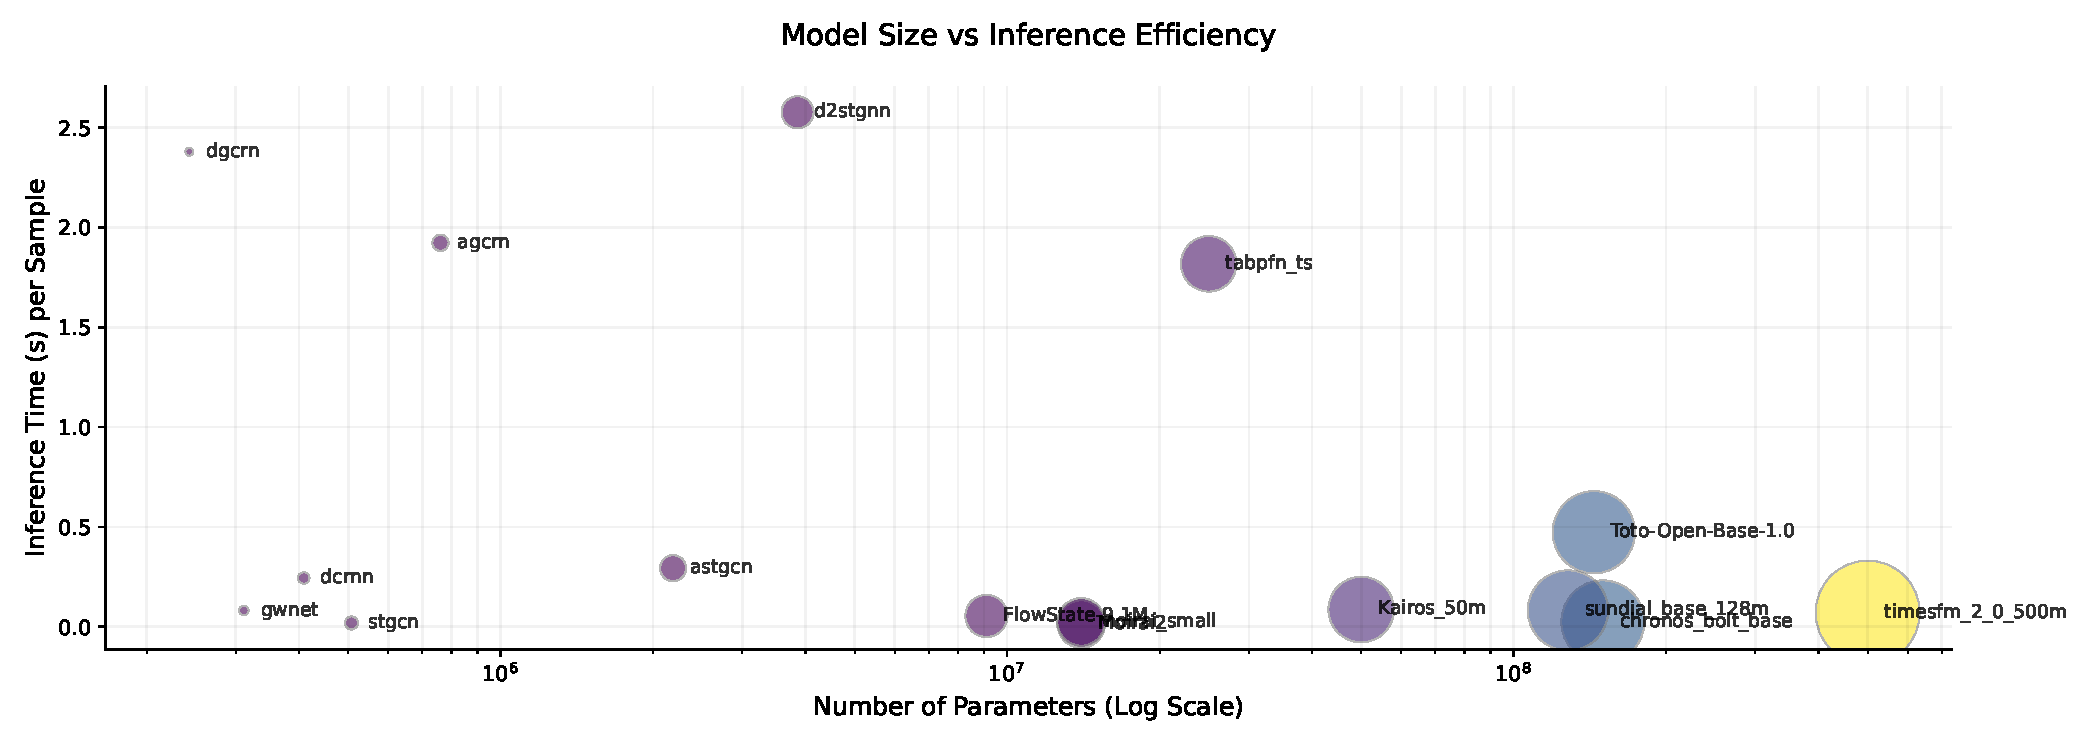
\includegraphics[width=1\linewidth]{images/time_interval/model_efficiency_chart (1).pdf}
    \caption{Model size vs.\ inference latency. Each point shows a model’s parameter count (x-axis, log scale) and average wall-clock inference time per sample (y-axis). Lower-left indicates better efficiency. Note that Spatiotemporal GNNs typically produce a \emph{full-graph} forecast in one forward pass. In contrast, univariate foundation models forecast \emph{per sensor series} and can run asynchronously as soon as a sensor’s latest reading arrives; network-wide latency depends on how many sensors are queried and the available batch/edge parallelism.}
    \label{fig:model_efficiency}
\end{figure*}
\subsection{Compute Cost and Efficiency Analysis}
\label{sec:efficiency}
\begin{figure}[t]
    \centering
    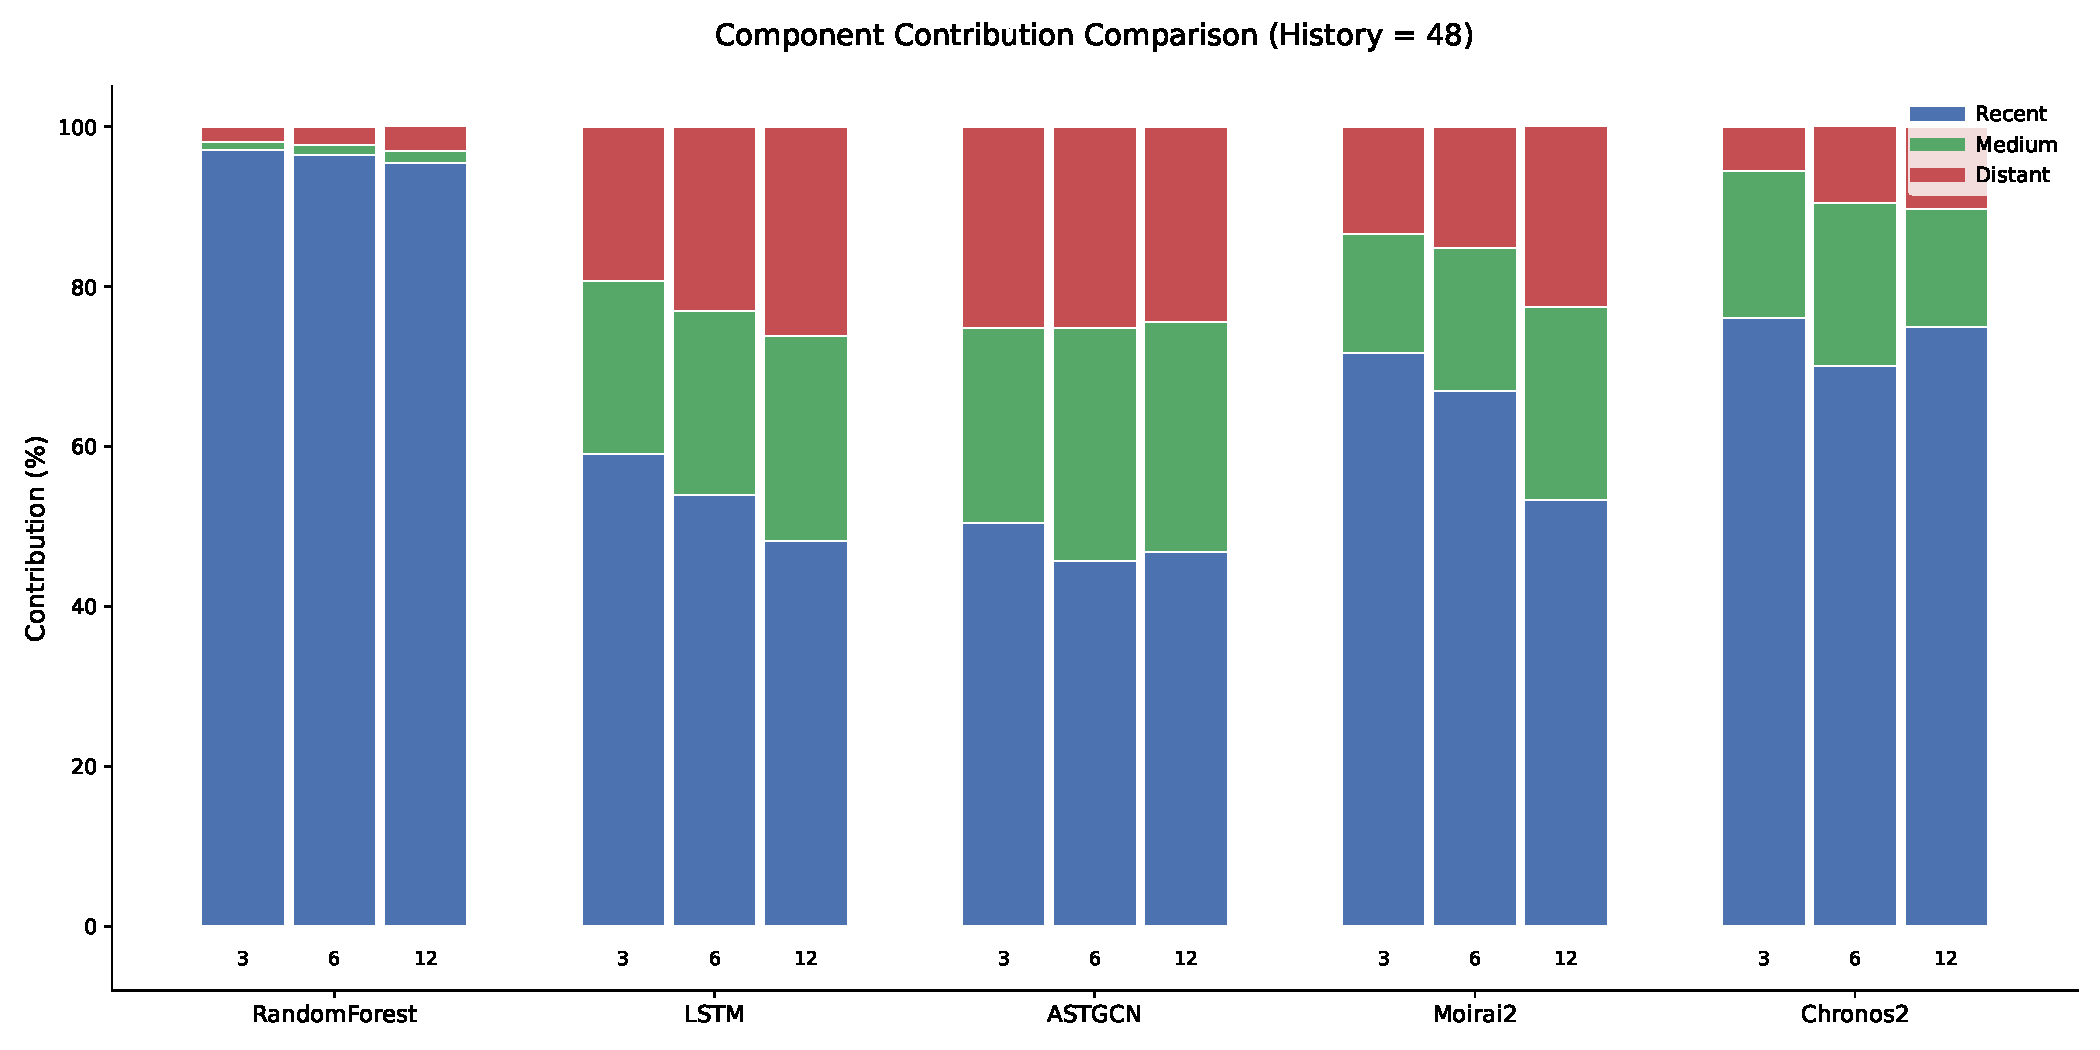
\includegraphics[width=\linewidth]{images/SHAP/history_48 (3).pdf}
    \caption{\textbf{Temporal-scale contribution (History $L{=}48$, 12h).} We aggregate absolute SHAP values over three contiguous lag groups (Recent / Medium / Distant) and normalize them to sum to 100\% for each model and horizon. Bars correspond to horizons $H\in\{3,6,12\}$.}
    \label{fig:shap_his48}
    \vspace{-0.3in}
\end{figure}




Deployment depends on system constraints as much as accuracy. Fig.~\ref{fig:model_efficiency} reports parameter
count versus per-inference latency, but note that model families produce different output granularities:
STGNNs generate a full-graph forecast in one forward pass, whereas univariate TSFMs forecast per sensor series.
As a rule of thumb, network-wide latency for TSFMs scales as $(N/B)\,t_{\text{uni}}$ (for $N$ sensors and batch
parallelism $B$), while STGNN cost is $\approx t_{\text{GNN}}$, implying that STGNNs amortize well for scheduled
network-wide forecasting, whereas TSFMs are better matched to event-triggered or sparse-query (edge/near-edge)
settings with asynchronous updates. Because ``end-to-end network time'' is heavily confounded by deployment
topology and batching, we report per-inference latency, which is reproducible and can be composed into
deployment-specific throughput.



% Deployment in intelligent transportation systems depends not only on accuracy but also on inference cost and
% system constraints. Figure~\ref{fig:model_efficiency} reports parameter count versus average inference time per
% sample. Importantly, these measurements reflect different \emph{output granularities}: spatiotemporal GNNs
% typically output a network-wide (full-graph) forecast in one forward pass, while univariate foundation models
% (e.g., Moirai2/Chronos/TimesFM) forecast per sensor series, requiring repeated inference to obtain
% network-level predictions (or large-batch parallelism when memory permits).

% This distinction yields a practical break-even rule of thumb. Let $t_{\text{GNN}}$ denote the time for one
% full-graph forward pass and $t_{\text{uni}}$ the time for one per-series forward pass. For $N$ sensors and
% effective batch parallelism $B$, univariate network-wide latency scales as $\approx (N/B)\,t_{\text{uni}}$,
% whereas the GNN cost remains $\approx t_{\text{GNN}}$. Thus:

\begin{keydiscovery1}
 \emph{Takeaway:}
 Even moderately slower GNNs can be competitive
when forecasts must be produced for many sensors on a fixed schedule, while univariate models are naturally
suited to event-triggered or sparse-query settings.  
\end{keydiscovery1}


% The figure also highlights that parameter count is a weak proxy for latency: compact GNNs can be slow due to
% recurrent/diffusion operators or dynamic graph learning, whereas very large transformers can remain efficient
% through optimized dense kernels. Finally, GNN deployments introduce a synchronization barrier---forming a full-graph
% snapshot requires waiting for all sensors at a timestamp (handling stragglers and missing values), while per-series
% inference supports asynchronous updates. These system considerations become even more pronounced under \emph{edge} or \emph{near-edge} deployment.
% When computation is pushed closer to sensors, the dominant requirement is often low-latency \emph{per-sensor}
% (or per-corridor) prediction under intermittent connectivity, rather than synchronized network-wide forecasting.
% In this regime, univariate transformer forecasters can be particularly attractive: they support lightweight,
% asynchronous updates and can exploit highly optimized dense-kernel inference on modern edge accelerators.
% This is also why we do not report a single ``end-to-end time for forecasting the entire network'': such a number
% is heavily confounded by the deployment topology (centralized vs.\ edge), batching strategy, and the set of queried
% sensors. Instead, we report \emph{per-inference} latency, which is reproducible and can be composed into a
% deployment-specific throughput estimate under the desired batching and edge/central execution model.

%These results motivate reporting both per-series and per-snapshot latency,
%along with end-to-end freshness under asynchronous arrivals.


\subsection{Predict Time Interval Analysis}


To understand \emph{when} models succeed or fail beyond aggregate metrics, we stratify errors by hour-of-day
and report mean absolute error (MAE) averaged across sensors within each hourly bin
(Figs.~\ref{fig:ASTGCN_hourly_mean_abs_error}--\ref{fig:Moiria2_hourly_mean_abs_error}).
The resulting diurnal profiles reveal complementary failure modes. ASTGCN shows higher errors during
low-demand late-night periods (e.g., around 02:00), which is consistent with potential sensitivity to
\emph{zero-inflated} regimes where small, spatially propagated biases can accumulate across many nodes.
In contrast, Moirai2 is comparatively stable overnight but its error increases sharply during
\emph{regime transitions}, most notably the morning ramp-up (05:00--08:00) and the evening peak, when traffic
changes rapidly. Taken together, these plots suggest that average MAE conflates qualitatively different sources of error (near-zero stability vs.\ transition dynamics), motivating regime-aware reporting (overnight vs.\ peak/transition)
and modeling choices that explicitly handle both zero-inflation and abrupt change-points.
\begin{keydiscovery1}
    \textit{Takeaway:}
Diurnal error profiles show a clear regime-dependent trade-off: the graph model  is more vulnerable in
near-zero overnight regimes ( due to spatially propagated bias under zero-inflation), while the foundation
model is more stable in low-flow periods but degrades during rapid ramp-up/peak transitions. %Hence,
%average MAE masks distinct failure modes, and evaluation/model choice should be conditioned on regime
%(overnight vs.\ transition/peak) rather than relying on a single aggregate score.
\end{keydiscovery1}





% -------------------------
% \section{Analysis}
% \label{sec:analysis}

% \subsection{Comparing model families}
% \begin{itemize}[leftmargin=1.2em]
%   \item \textbf{Traditional ML and ensembles:} computationally efficient; simple mean ensembles are strong, robust baselines with fast training.
%   \item \textbf{GNNs:} strong for short horizons due to localized spatiotemporal correlation modeling; serve as classic strong baselines.
%   \item \textbf{Foundation models:} more robust for long horizons and cross-dataset generalization; competitive under zero/few-shot or light tuning.
% \end{itemize}

% \subsection{Scale and generalization effects}
% \TODO{Analyze how performance changes from CA$\rightarrow$GLA$\rightarrow$GBA$\rightarrow$SD; if available, include cross-region train/test transfer experiments.}

% \subsection{Compute cost and efficiency}
% \TODO{Add training/inference cost comparisons: wall-clock time, GPU memory, throughput; emphasize ML/ensemble efficiency, GNN GPU training needs, and foundation inference costs vs reusable pretraining benefits.}

\subsection{Forecasts Change with Horizon and Context}
\label{sec:interpretability}

% (Tip) Filenames with spaces/parentheses may break LaTeX; consider renaming
% history_48 (3).pdf -> history_48.pdf for robustness.



% Rather than treating SHAP purely as an explanation tool, we use grouped temporal attributions
% (Figs.~\ref{fig:shap_his48}--\ref{fig:shap_his96}) to diagnose \emph{why} model performance changes with forecasting
% horizon and available history, and \emph{when} different model classes are expected to work best.
% Across models, increasing the horizon shifts importance away from \textit{Recent} toward longer lags, reflecting
% that medium-horizon forecasts rely more on stable structure (e.g., periodicity) than on short-term persistence.
% However, model classes differ sharply in how they realize this shift: (i) the tabular \textbf{RandomForest} remains
% strongly myopic (dominated by \textit{Recent} under $L{=}48$, and still heavily \textit{Recent} under $L{=}96$),
% which is consistent with its typical strength at very short horizons but limited long-range extrapolation;
% (ii) temporal neural models such as \textbf{LSTM} and graph-based \textbf{ASTGCN} exhibit a clearer rebalancing toward
% \textit{Medium}/\textit{Distant} as $H$ increases, indicating a more explicit multi-timescale strategy; and
% (iii) foundation models (\textbf{Moirai2}, \textbf{Chronos2}) retain a strong near-term reliance but increase their
% use of longer history as horizons extend, suggesting robustness from short-term signals with selective long-range
% conditioning.


% Extending the context from $L{=}48$ (12h) to $L{=}96$ (24h) induces a qualitative shift: importance is reallocated
% from \textit{Medium} to \textit{Distant} lags for several architectures, most visibly for \textbf{ASTGCN}, whose
% \textit{Distant} contribution grows substantially once a full-day context is available (Fig.~\ref{fig:shap_his96}).
% This pattern is consistent with a practical mechanism in traffic: once the input spans a full diurnal cycle,
% models can anchor predictions using daily periodicity, improving stability at longer horizons.

% A second, complementary observation is that {foundation models remain more ``recent-driven'' overall}:
% their grouped attributions place a larger fraction of mass on the \textit{Recent} window than spatiotemporal GNNs,
% even when $L{=}96$. This implies a stronger reliance on short-term cues and local temporal continuity, with
% comparatively weaker dependence on mid/remote history. Such a reliance profile helps explain the diurnal error
% pattern observed in Figure~\ref{fig:Moiria2_hourly_mean_abs_error}: during the morning ramp-up, traffic transitions rapidly from uncongested to congested regimes, and when the recent context is dominated by low/near-zero flow, purely temporal near-term cues can be
% weakly informative about an imminent regime change. In contrast, graph-based models that allocate more weight to
% longer lags (and can implicitly exploit spatial precursors) are better positioned to anticipate the onset of
% congestion, narrowing the gap precisely during transition windows. This recent-driven reliance also enables {faster response} to abrupt changes: because transformer foundation models condition heavily on the most recent observations, their forecasts can adapt quickly as soon as
% new measurements arrive, which is particularly beneficial under asynchronous or event-triggered updates.


% Taken together, grouped temporal contributions offer an actionable lens for model selection and for explaining why
% accuracy rankings can change with $(L,H)$ under a fixed protocol: recent-driven models tend to excel in stable regimes and short horizons, whereas models that effectively leverage daily-scale history (and/or spatial coupling) are more reliable as horizons extend and when periodic structure or regime transitions dominate.


We use grouped temporal SHAP (Figs.~\ref{fig:shap_his48}--\ref{fig:shap_his96}) to explain \emph{why} rankings
change with horizon and available history. As $H$ increases, all models shift importance away from \textit{Recent}
toward longer lags, consistent with medium-horizon forecasts relying more on stable structure (e.g., periodicity).
Model classes differ in how strongly they make this shift: \textbf{RandomForest} remains largely myopic, while
\textbf{LSTM}/\textbf{ASTGCN} reweight more clearly toward \textit{Medium}/\textit{Distant}. Foundation models
(\textbf{Moirai2}/\textbf{Chronos2}) stay more recent-driven overall, but selectively increase long-lag usage as
$H$ grows.
Increasing context from $L{=}48$ to $L{=}96$ produces a qualitative change for several models, most notably
\textbf{ASTGCN}, which reallocates attribution from \textit{Medium} to \textit{Distant} once a full diurnal cycle is
available (Fig.~\ref{fig:shap_his96}), consistent with anchoring on daily periodicity for improved stability.

By contrast, foundation models keep a larger share of mass on \textit{Recent}, which helps explain their diurnal
profile: they are stable overnight but can spike during morning ramp-up when recent history is near-zero and
weakly predictive of an imminent regime change. This same recent-driven conditioning also enables faster response
to shocks as soon as new measurements arrive, benefiting asynchronous or event-triggered updates. Overall,
grouped attributions provide an actionable lens for model choice: recent-driven models tend to work well in stable
regimes and short horizons, while models that exploit diurnal-scale history and/or spatial coupling are more
reliable as horizons extend and during regime transitions.
\begin{keydiscovery1}
    \textit{Takeaway:}
Recent-driven foundation models enable fast, responsive
updates but are more prone to miss abrupt ramp-ups, whereas models that allocate more mass to diurnal-scale history
(and/or spatial coupling) are better suited for transition-heavy periods.
\end{keydiscovery1}

\begin{table}[t]
\centering
\caption{Incident-conditioned forecasting on SD collision windows. ML: machine learning regressors; DL: task-trained deep learning baselines; FM: pretrained foundation models.}
\label{tab:model_comparison}
\resizebox{\linewidth}{!}{
\begin{tabular}{cc|cc|cc|cc}
\toprule
\multirow{2}{*}{\textbf{Category}} & \multirow{2}{*}{\textbf{Method}}
& \multicolumn{2}{c|}{\textbf{$H{=}3$}} 
& \multicolumn{2}{c|}{\textbf{$H{=}6$}} 
& \multicolumn{2}{c}{\textbf{$H{=}12$}} \\
\cmidrule(lr){3-4}\cmidrule(lr){5-6}\cmidrule(lr){7-8}
 &  & \textbf{MAE} & \textbf{RMSE} & \textbf{MAE} & \textbf{RMSE} & \textbf{MAE} & \textbf{RMSE} \\
\midrule
\multirow{3}{*}{ML}
& Naive              & 29.82 & 46.20 & 42.46 & 66.51 & 67.49 & 102.72 \\
& Random Forest      & 26.19 & 39.55 & 33.65 & 50.93 & 39.76 & 61.99 \\
& Ensemble Mean      & 24.39 & 36.58 & 31.64 & 46.83 & \textemdash & \textemdash \\
\midrule
\multirow{2}{*}{DL}
& LSTM               & 25.25 & 40.12 & 26.18 & 40.27 & 28.79 & 43.60 \\
& ASTGCN             & 27.41 & 42.98 & 28.62 & 43.93 & 30.46 & 48.57 \\
\midrule
\multirow{6}{*}{FM}
& Chronos-Bolt  & 17.29 & 28.16 & 18.33 & 30.18 & 20.29 & 33.79 \\
& Sundial & 16.55 & 27.40 & 17.97 & 29.69 & 21.01 & 34.36 \\
& TimesFM   & 16.38 & 27.02 & 17.12 & 28.71 & 18.77 & 31.87 \\
& Moirai-Small       & 29.68 & 45.06 & 38.41 & 59.53 & 55.26 & 85.46 \\
& FlowState    & 16.90 & 27.54 & 17.57 & 29.00 & 19.27 & 31.96 \\
& Kairos      & 18.34 & 28.97 & 20.21 & 32.31 & 23.94 & 39.49 \\
\bottomrule
\end{tabular}
}
\vspace{1mm}
%\footnotesize{\textit{Note.} \textemdash\ denotes missing or unavailable measurements for that setting.}
\end{table}



\begin{figure}[t]
    \centering
    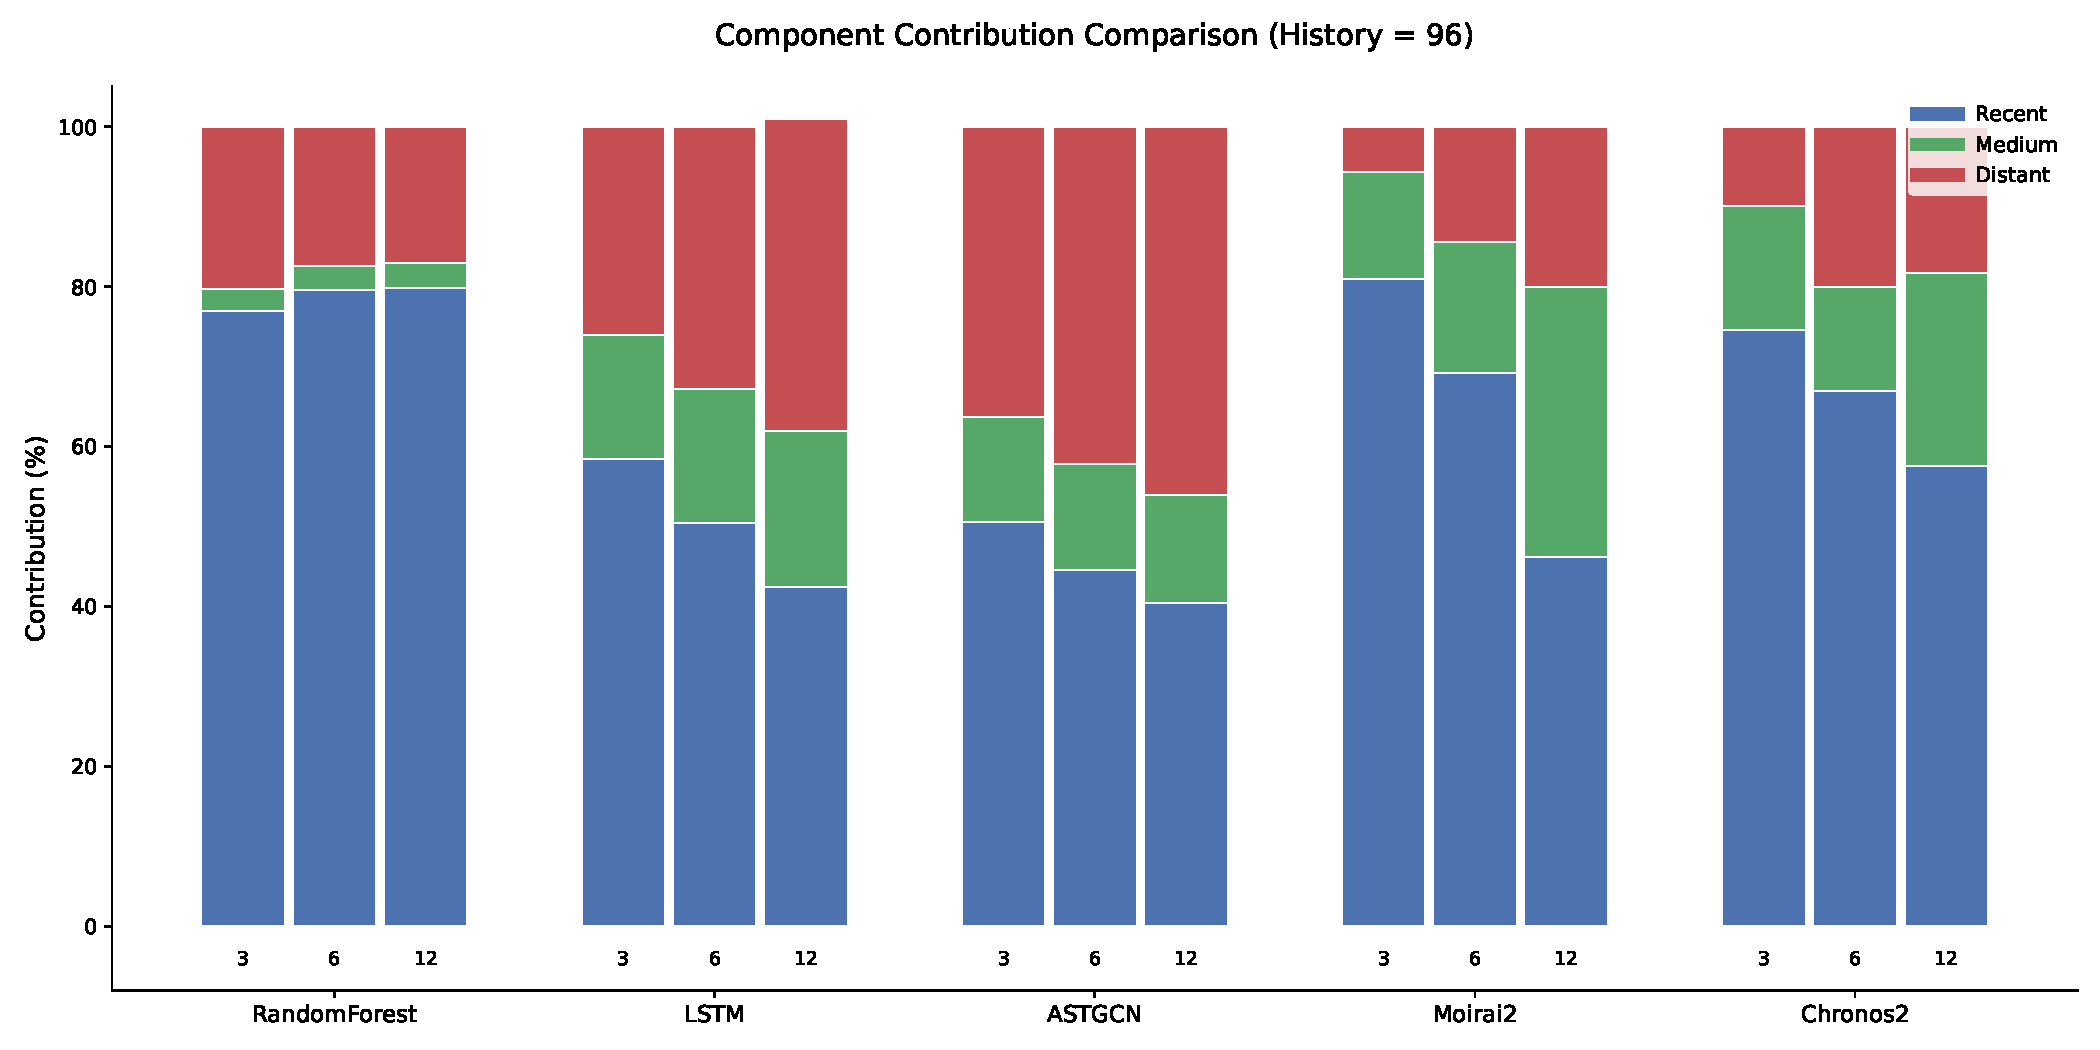
\includegraphics[width=\linewidth]{images/SHAP/history_96.pdf}
    \caption{\textbf{Temporal-scale contribution (History $L{=}96$, 24h).} Same grouped SHAP analysis as Fig.~\ref{fig:shap_his48}, but with a full-day context that exposes diurnal periodic signals.}
    \label{fig:shap_his96}
    \vspace{-0.3in}
\end{figure}
\subsection{Incident-conditioned forecasting reveals regime-specific inductive biases}
\label{sec:incident}

To stress-test robustness under non-stationary disruptions, we evaluate models on an incident-conditioned
setting using San Diego collision records: for each collision, we select the six sensors most correlated with
event metadata and forecast post-collision traffic for horizons $H\in\{3,6,12\}$.
Table~\ref{tab:model_comparison} shows that persistence-style baselines degrade sharply with horizon
(Naive MAE: 29.82$\rightarrow$67.49), confirming that collision windows constitute a strong distribution shift.

Pretrained foundation models dominate across horizons: \texttt{TimesFM} attains the lowest MAE at all
three horizons (16.38/17.12/18.77), with \texttt{FlowState-9.1M} and \texttt{Chronos-Bolt-Base} close behind.
Compared to the graph-based \texttt{ASTGCN}, \texttt{TimesFM} reduces MAE by $\approx$38--40\% and RMSE by
$\approx$34--37\%, indicating substantially better adaptation to post-incident dynamics.

These results align with our earlier temporal-reliance findings: foundation models tend to be more
\emph{recent-driven}, which allows forecasts to update quickly as soon as new post-incident measurements arrive
(i.e., faster response under asynchronous/event-triggered inference). In contrast, \texttt{ASTGCN} underperforms
even a temporal-only \texttt{LSTM} (5--9\% lower MAE), suggesting that a static message-passing prior can be
suboptimal for localized, directional shocks. Spatial aggregation encourages global smoothness, which may dampen
abrupt changes and yield conservative but biased predictions during incident recovery.
Overall, incident-conditioned forecasting provides a targeted robustness
benchmark and motivates event-aware temporal priors and directionality-aware spatial modeling (e.g., dynamic or
directed graphs).
%Finally, we observe substantial heterogeneity within foundation models (e.g., \texttt{Moirai-Small} is close to
%Naive), implying that robustness to incident regimes depends on pretraining priors and inference configurations
%rather than ``foundation'' status alone. 

\begin{keydiscovery1}
    \textit{Takeaway:}
Robust post-incident recovery forecasting requires event-aware temporal dynamics and directionality-aware (not
purely global-smoothing) spatial modeling.
\end{keydiscovery1}

% \subsection{Qualitative case studies}
% \TODO{Show real vs predicted curves with SHAP heatmaps for selected sensors and time periods.}

% % -------------------------
% \section{Ablations and Robustness}
% \label{sec:ablations}

% \begin{itemize}[leftmargin=1.2em]
%   \item \textbf{Ensemble strategies:} mean vs median vs weighted mean; effect of ensemble pool size and diversity.
%   \item \textbf{Data frequency:} robustness under frequency changes (if supported) or resampling variations.
%   \item \textbf{Training time span:} effect of training years / history length.
%   \item \textbf{Hyperparameter sensitivity:} key knobs for GNNs/foundation models and their stability.
%   \item \textbf{Missingness/noise:} robustness under controlled masking or perturbation (if available).
% \end{itemize}

% % -------------------------
% \section{Limitations and Future Work}
% \label{sec:limitations}

% \begin{itemize}[leftmargin=1.2em]
%   \item \textbf{Domain scope:} traffic is central but not exhaustive; extend the protocol to other spatiotemporal domains.
%   \item \textbf{Spatial interpretability:} current analysis focuses on temporal attribution; future work should include sensor/edge-level explanations.
%   \item \textbf{Real-time deployment:} latency, drift detection, and continual adaptation remain challenging.
% \end{itemize}

% -------------------------

% -------------------------
\section{Conclusion}
\label{sec:conclusion}

We present \LargeST{}, a unified benchmark for large-scale traffic flow forecasting that standardizes data processing, chronological splits, horizons, and metrics, enabling fair comparison across classical ML baselines, spatiotemporal GNNs, and time-series foundation models.

% Lightweight ML ensembles are strong, low-cost baselines.
% GNNs remain highly competitive at short horizons, but require synchronized full-graph snapshots and can be
% sensitive to missing/straggler sensors. Foundation models often achieve the best overall accuracy and
% horizon stability, and their per-series inference supports asynchronous and edge-friendly deployment.
% Their stronger reliance on recent history yields faster updates, but can be brittle during abrupt regime
% transitions.

Our results provide several practical takeaways. Foundation models often achieve the best overall accuracy and
horizon stability, and their per-series inference supports asynchronous and edge-friendly deployment. Beyond point metrics, we introduced deployment- and regime-aware diagnostics—per-inference latency with explicit
full-graph vs.\ per-series accounting, diurnal error stratification, grouped-lag SHAP temporal reliance, and an
incident-conditioned evaluation using collision records—to explain \emph{why} rankings change with $(L,H)$ and
\emph{when} each family is preferable. Together, these results motivate future work on hybrid designs that combine
rapid local updates with directional, event-aware spatial reasoning, as well as evaluation protocols that report
performance by operational regime rather than a single aggregate score. We release the end-to-end pipeline to
enable reproducible comparisons and to support deployment-oriented model selection in practice.


% -------------------------
% Appendix: Command cookbook template (optional)
% -------------------------



% -------------------------
% Bibliography (optional)
% -------------------------
\bibliographystyle{tmlr}
\bibliography{ref}

\clearpage
\appendix


\begin{table*}[t]
\centering
\caption{LargeST subset statistics used in this benchmark (year 2019, resampled to 15-minute).}
\label{tab:datasets}
\begin{tabular}{lrrrr}
\toprule
Subset & \#Sensors ($N$) & \#Timesteps ($T$) & Duration & Notes \\
\midrule
CA  & 8{,}600 & 35{,}040 & 2019 (1 year) & State-wide California mainline sensors \\
GLA & 3{,}834 & 35{,}040 & 2019 (1 year) & Greater Los Angeles (5 counties) \\
GBA & 2{,}352 & 35{,}040 & 2019 (1 year) & Greater Bay Area (11 counties) \\
SD  & 716     & 35{,}040 & 2019 (1 year) & San Diego county \\
\bottomrule
\end{tabular}
\end{table*}


% \section{Experimental Protocol}
% \label{sec:protocol}



% To ensure a rigorous and fair evaluation across disparate model families, we establish a unified experimental protocol. This framework eliminates confounding factors such as mismatched data splits, inconsistent normalization, or varying horizon definitions, ensuring that performance gains are attributable solely to modeling innovations.

% \subsection{Unified Preprocessing}
% We standardize the data pipeline to maintain consistency across traditional ML, GNNs, and foundation models. The preprocessing steps are as follows:
% \begin{itemize}[leftmargin=1.2em]
%     \item \textbf{Time Alignment and Resampling:} Raw 5-minute traffic readings are aggregated into 15-minute windows (96 steps/day). We utilize data from the year 2019 to mitigate COVID-era distribution shifts while maintaining computational feasibility for high-complexity baselines.
%     \item \textbf{Normalization:} We apply Z-score normalization per sensor based on training set statistics. This ensures stable gradient flow in neural architectures and uniform feature scaling for linear models.
%     \item \textbf{Missing-value Handling:} Linear interpolation is utilized for short-term gaps, while persistent missing values are masked during loss computation to prevent optimization bias.
% \end{itemize}



% \subsection{Benchmark Implementation and Entry Points}
% The benchmark is implemented as a modular framework to facilitate end-to-end reproducibility. We provide standardized execution modules for each component of the pipeline:
% \begin{itemize}[leftmargin=1.2em]
%     \item \textbf{Evaluation Core:} A unified interface handles dataset loading, windowing logic, and the computation of standardized metrics (MAE, RMSE, MAPE).
%     \item \textbf{Model Execution Modules:} Standardized entry points are provided for traditional machine learning, spatiotemporal GNNs, and time-series foundation models to ensure they are trained and evaluated under identical conditions.
%     \item \textbf{Interpretability Pipeline:} A dedicated SHAP-based module enables the generation of temporal attribution profiles and visualization of model reliance patterns.
% \end{itemize}


% \subsection{Seeds and Repeatability}
% To account for stochasticity in model initialization and optimization, we fix a consistent set of random seeds across all experiments. For stochastic methods—particularly GNNs—we report the aggregate performance ($\text{mean} \pm \text{std}$) over \TODO{number} independent runs. This ensures the statistical robustness of the reported results across the CA, GLA, GBA, and SD subsets.
% -------------------------

\begin{table*}[t]
\centering
\caption{Method families and evaluated models in our benchmark.}
\label{tab:method_families}
\begin{tabular}{p{2.7cm}p{9.0cm}}
\toprule
Family & Evaluated methods and characteristics \\
\midrule
Simple baselines
& \textbf{HL} (historical last / persistence); \textbf{Naive}; \textbf{seasonal\_naive} (lightweight sanity checks; strong periodicity prior). \\

Traditional ML
& \textbf{linear\_regression}, \textbf{ridge} (lag-feature regression); \textbf{random\_forest} (nonlinear tabular baseline);
\textbf{lightgbm} (gradient boosting on lag features; CPU-friendly). \\

Ensembles
& \textbf{median}, \textbf{mean}, \textbf{weighted} ensembles of \textbf{seasonal\_naive + ridge + linear\_regression + random\_forest}
(low-cost robustness; mean is a special case of weighted with uniform weights). \\

RNN-based
& \textbf{LSTM} (temporal-only neural baseline; trained per task). \\

Spatiotemporal GNNs
& \textbf{DCRNN}, \textbf{AGCRN}, \textbf{STGCN}, \textbf{GWNET}, \textbf{ASTGCN}, \textbf{STTN}, \textbf{STGODE}, \textbf{DSTAGNN}, \textbf{DGCRN}, \textbf{D2STGNN}
(full-graph, graph-aware spatiotemporal modeling; retrained on each subset). \\

Foundation / large pretrained models
& \textbf{Chronos-2}, \textbf{Chronos-Bolt}, \textbf{Moirai-2}, \textbf{Moirai-Small}, \textbf{TimesFM} (\texttt{timesfm\_2\_0\_500m}),
\textbf{Kairos}, \textbf{sundial\_base\_128m}, \textbf{FlowState-9.1M}
(pretrained forecasters, typically per-series inference; strong transfer under a unified protocol). \\
\bottomrule
\end{tabular}
\end{table*}



\section{Dataset and Tasks}
\label{sec:data}

\textit{LargeST subsets}
LargeST is a large-scale traffic forecasting benchmark sourced from CalTrans PeMS mainline loop
detectors in California \citep{liu2023largest}. It provides four real-world subsets with increasing spatial
scale: {CA} (state-wide California; 8,600 sensors), {GLA} (Greater Los Angeles; five counties; 3,834 sensors),
{GBA} (Greater Bay Area; eleven counties; 2,352 sensors), and {SD} (San Diego county; 716 sensors). Each sensor is
accompanied by metadata such as geographic coordinates, district, highway, travel direction, and number
of lanes.
The original LargeST release provides 5-minute readings from 2017--2021. Following
the standard experimental setup used in LargeST, we aggregate 5-minute readings into {15-minute}
windows (96 steps/day) and use {the year 2019} to reduce COVID-era distribution shift and to make
slower baselines feasible, as detailed in Table~\ref{tab:datasets}. 


\textit{Data prepare.}
We aggregate 5-minute readings into non-overlapping 15-minute windows. Unless stated otherwise, the
target is traffic \emph{flow}. We apply per-sensor $z$-score normalization using statistics computed \emph{only on the training split}.
The same training statistics are applied to validation and test, preventing information leakage across
time. We generate supervised instances using a stride-$H$ sliding window over time. For each $(L,H)$, an input
consists of the most recent $L$ steps and the target consists of the next $H$ steps.




\textit{Operational interpretation.}
At 15-minute resolution, horizons $H=3/6/12$ correspond to 45 minutes / 1.5 hours / 3 hours
ahead. Rather than fixing a single context length across all models, we follow each method's recommended best-practice configuration and select the input length that yields its best validation performance if accessible. This avoids penalizing methods whose design assumes a particular receptive field, while keeping the prediction targets identical across approaches. For methods that naturally output probabilistic forecasts, we compute deterministic metrics using the predictive mean. We use time-based splits, training on the first 60\% of the data points if needed, and fix the sliding window size for a fairness and best-practice configuration.


\textit{Forecasting task}
We study multi-step traffic flow forecasting on a directed sensor graph. Let
$X \in \mathbb{R}^{T \times N \times C}$ denote traffic measurements over time ($T$), sensors ($N$), and
channels ($C$). In our benchmark, we forecast {traffic flow} (typically $C=1$).
Given a context window of length $L$,
$\mathcal{X}_{t} = X_{t-L+1:t}$, the model predicts the next $H \in \{3, 6, 12\}$ steps:
$\hat{X}_{t+1:t+H} = f(\mathcal{X}_{t})$.


\textit{Interpretability and actionable insights}
\label{sec:insights}
Beyond accuracy, we characterize \emph{how} different model families use historical context via
model-agnostic temporal attribution (SHAP) \citep{lundberg2017shap}. We compute attributions on the same
deterministic quantity used for evaluation (predictive mean/median for probabilistic models) and
aggregate attributions across sensors and time. This yields concise summaries of which lags (e.g., recent
history vs.\ periodic components) dominate predictions under different horizons and subsets, enabling
insights directly relevant to deployment and monitoring.


%\appendix
% \section{Additional Benchmark Details}
% \label{sec:appendix_setup}

% \subsection{Data preprocessing}
% \label{sec:appendix_preprocess}
% We aggregate 5-minute readings into non-overlapping 15-minute windows (96 steps/day).
% Unless stated otherwise, the prediction target is traffic \emph{flow}.
% We apply per-sensor $z$-score normalization using statistics computed \emph{only} on the training split; the same
% training statistics are applied to validation and test to prevent temporal leakage.
% Supervised instances are generated by a sliding window over time: each input contains the most recent $L$ steps and
% each target contains the next $H$ steps.

% \subsection{Splits and windowing}
% \label{sec:appendix_splits}
% We use chronological (time-based) splits with a 60/20/20 train/validation/test partition over the 2019 timeline.
% For each horizon $H$, windows are extracted with a fixed stride (default stride=1) to maximize sample usage and to
% keep evaluation consistent across model families. All preprocessing, splits, and metrics are shared across methods.

% \subsection{Context length selection and probabilistic outputs}
% \label{sec:appendix_context_prob}
% To avoid conflating architectural assumptions with protocol choices, we select each model's input context length
% based on validation performance from a common candidate set. This follows best-practice usage for models that
% assume particular receptive fields (e.g., seasonal or long-context designs) while preserving identical prediction
% targets across methods.
% For methods that output probabilistic forecasts, we report point-forecast metrics using the predictive mean.

% \subsection{Graph topology (for graph-based models)}
% \label{sec:appendix_graph}
% For GNN-based methods, we follow the \textsc{LargeST} released graph construction, which models the sensor network as
% a directed graph derived from road-network distances and a thresholded Gaussian kernel \citep{liu2023largest}.


% -------------------------
% -------------------------
\section{Models and Baselines}
\label{sec:models}

% --- Local definitions (safe even if defined elsewhere) ---
\providecommand{\freq}{15\text{ min}}
\providecommand{\ctxset}{\{48, 98, 196, 336, 720\}}
\providecommand{\hzset}{\{3, 6, 12, 48\}}

As shown in Table~\ref{tab:method_families}, we benchmark a diverse set of forecasting methods spanning (i) ML baselines such as Ridge/Random Forest/boosting methods, (ii) established spatiotemporal GNN architectures (e.g., DCRNN, AGCRN, STGCN, GWNET, and variants), and (iii) foundation models (Chronos, Moirai2, TimesFM, etc.) leveraging large-scale pretraining.





\subsection{Traditional baselines}
Traditional statistical and ML baselines recast forecasting into supervised regression using lag-based features.
Given the last $L$ observations from a single sensor, we construct a feature vector of recent lags and train a
regressor to predict the next step. Multi-step forecasting is obtained via iterative roll-out: the model predicts
one step ahead, then the predicted value is appended to the context and used to predict subsequent steps up
to horizon $H$.

\textit{Seasonal Naive.}
Seasonal Naive is a transparent baseline that repeats a seasonal pattern (e.g., the same time-of-day
from a previous cycle). It provides a strong sanity check in traffic settings where periodicity is prominent,
and it requires no model training.

\textit{Linear Regression and Ridge Regression.}
Linear regression provides a minimal baseline. Ridge regression adds $\ell_2$ regularization, which is
particularly helpful when using long contexts (large $L$) where lag features may be highly correlated.

\textit{Tree ensembles: Random Forest (RF).}
RF aggregates many decision trees trained on bootstrapped samples to reduce variance and capture non-linear
interactions among lag features. RF is robust with minimal tuning and often performs competitively as a
low-cost baseline.

\textit{Boosting: LightGBM/GBM and XGBoost (XGB).}
Gradient-boosted decision trees typically provide strong accuracy on tabular features with good regularization.
We include both LightGBM-style gradient boosting and XGBoost as representative boosting frameworks, offering
a strong accuracy--efficiency trade-off in CPU-based forecasting.

\textit{Ensemble baselines}
Ensembles improve robustness by combining forecasts from multiple base models. Let
$\{\hat{\mathbf{x}}^{(k)}\}_{k=1}^K$ be the $H$-step forecasts from $K$ models. We use a weighted ensemble:
\[
\hat{\mathbf{x}}^{\text{ens}}=\sum_{k=1}^K w_k \hat{\mathbf{x}}^{(k)}, \qquad
\sum_{k=1}^K w_k=1,\;\; w_k\ge 0,
\]
where weights are chosen on the validation set. The mean ensemble is a special case with uniform weights
$w_k=1/K$. We employ a weighted ensemble forecasting approach that combines four base models: a seasonal naïve model, ridge regression, linear regression, and a random forest. 
The final ensemble prediction is computed as a convex combination of the individual model forecasts, with weights $(0.15, 0.30, 0.20, 0.35)$ assigned to the seasonal naïve, ridge regression, linear regression, and random forest models, respectively. 
This ensemble configuration is denoted as
\texttt{ensemble\_weighted}.


\subsection{Neural baseline}
\textit{Feedforward forecaster.}
We include a lightweight feedforward neural network (multi-layer perceptron) as a minimal deep-learning baseline.
The model maps a length-$L$ context window to multi-step predictions and serves as a reference point between
tabular ML and more structured spatiotemporal architectures. While simple, it can benefit from GPU acceleration
and provides a sanity check for whether non-linear representation learning alone improves over tree-based models.

\subsection{Spatiotemporal GNN baselines}
Spatiotemporal GNNs forecast jointly across sensors by combining graph-based spatial modeling with temporal
dynamics. They are particularly well-suited to traffic networks because spatial correlations arise from road
connectivity and shared congestion patterns. We include representative architectures along major design axes:

\textit{RNN-based graph forecasting (DCRNN, AGCRN, DGCRN).}
These models couple graph convolutions with recurrent temporal modeling to capture evolving traffic states.
DCRNN uses diffusion-style graph convolution integrated with gated recurrent units, while AGCRN learns an
adaptive graph structure to better fit sensor interactions. DGCRN further emphasizes dynamic correlations to
handle time-varying dependencies.

\textit{Temporal convolution (STGCN, GWNET).}
TCN-based approaches replace recurrence with dilated causal convolutions for parallelism and speed.
STGCN combines temporal convolutions with graph convolutions, while GWNET uses gated dilated convolutions
and graph propagation, often serving as a strong `classic'' baseline for traffic forecasting.

\textit{Attention-based spatiotemporal models (ASTGCN, STTN).}
Attention mechanisms can dynamically focus on informative sensors and timesteps.
ASTGCN introduces spatial and temporal attention atop convolutional blocks, while STTN employs transformer-style
attention to capture complex spatiotemporal dependencies.

\textit{Continuous-time dynamics (STGODE).}
STGODE models temporal evolution using neural ordinary differential equations, aiming to capture longer-range
dynamics via continuous transformations.

\textit{Dynamic-topology modeling (DSTAGNN, D2STGNN).}
These methods explicitly account for time-varying spatial dependencies, e.g., by constructing dynamic adjacency
representations or multi-faceted graph structures, which can be beneficial under non-stationary traffic regimes.

\subsection{Time-series foundation models}
Time-series foundation models are pretrained on large and diverse time-series corpora and can be applied to
new domains with limited or no task-specific training. In this benchmark we primarily evaluate them in
\emph{zero-shot} mode (direct inference on each sensor series), and when applicable we also consider light
adaptation settings. Their outputs are aligned to our $(L,H)$ grid; when probabilistic forecasts are produced,
we use the predictive mean for point-metric computation.

\textit{Chronos.}
Chronos is a transformer-based foundation model that casts forecasting into a sequence modeling problem and
supports multiple pretrained sizes. It provides a strong zero-shot baseline and often exhibits robust behavior
for longer horizons.

\textit{Moirai and Moirai2.}
Moirai-style models are universal forecasters trained across diverse datasets, designed to generalize across
domains and frequencies. We evaluate both Moirai and the updated Moirai2 variant, which can offer improved
robustness and longer-range dependency modeling.

\textit{TimesFM.}
TimesFM is a decoder-only transformer forecaster pretrained at scale, emphasizing efficient inference and
support for multiple context lengths. It serves as a representative industrial-grade foundation model baseline.

\textit{Additional pretrained baselines (Kairos, FlowState, TabPFN-TS).}
To broaden coverage, we also include additional pretrained approaches representing alternative modeling
paradigms: (i) multi-scale attention-based forecasting (Kairos), (ii) state-space / flow-inspired designs
(FlowState), and (iii) meta-learning / in-context tabular-style forecasting (TabPFN-TS). These methods expand
the foundation-model design space and help assess whether different pretraining and adaptation strategies
transfer to large-scale traffic data.




\begin{table*}[t]
\centering
\caption{Performance Comparison of Forecasting Methods (Los Angeles Data)}
\label{tab:performance_comparison_gla}
\resizebox{\textwidth}{!}{
\begin{tabular}{c|c|c|c|c|c|c|c|c|c|c|c|c|c}
\toprule
Category & Method & H3 MAE & H3 RMSE & H3 MAPE & H6 MAE & H6 RMSE & H6 MAPE & H12 MAE & H12 RMSE & H12 MAPE & Avg MAE & Avg RMSE & Avg MAPE \\
\midrule
\multirow{3}{*}{Simple Baselines}
& HL & 33.66 & 50.91 & 19.16\% & 56.88 & 83.54 & 34.85\% & 98.45 & 137.52 & 71.14\% & 59.58 & 86.19 & 38.76\% \\
& Naive & 22.94 & 35.71 & 10.66\% & 36.38 & 54.51 & 22.81\% & 52.54 & 80.26 & 36.84\% & 37.29 & 56.83 & 23.44\% \\
& Seasonal Naive & 35.96 & 62.29 & 17.59\% & 32.55 & 56.17 & 18.85\% & 45.96 & 76.53 & 25.01\% & 38.16 & 65.00 & 20.48\% \\
\midrule
\multirow{4}{*}{ML Baselines}

& Ridge & 20.62 & 32.97 & 10.11\% & 29.03 & 44.24 & 24.42\% & 41.03 & 92.36 & 39.09\% & 30.23 & 56.52 & 24.54\% \\
& Random Forest & 22.15 & 35.04 & 9.77\% & 28.20 & 43.97 & 17.16\% & 34.91 & 55.48 & 22.86\% & 28.42 & 44.83 & 16.60\% \\
& Linear Regression & 20.62 & 32.97 & 10.11\% & 166.65 & - & 70.24\% & 41.14 & 100.56 & 39.12\% & 76.13 & - & 39.82\% \\
& LightGBM & 23.32 & 35.70 & 10.83\% & 30.04 & 44.07 & 22.55\% & 38.63 & 57.92 & 31.05\% & 30.66 & 45.90 & 21.47\% \\
\midrule
\multirow{3}{*}{Ensembles}
& Median & 19.16 & 31.09 & 9.09\% & 24.90 & 37.79 & 18.95\% & 34.10 & 62.09 & 29.29\% & 26.05 & 43.66 & 19.11\% \\
& Mean & 19.66 & 31.07 & 9.83\% & 58.10 & - & 29.42\% & 33.19 & 61.58 & 28.06\% & 36.98 & - & 22.44\% \\
& Weighted & 19.28 & 30.53 & 9.41\% & 51.93 & - & 27.54\% & 33.12 & 61.29 & 28.33\% & 34.77 & - & 21.76\% \\
\midrule
\multirow{6}{*}{GNN-based}
& ASTGCN & 21.89 & 34.17 & 13.29\% & 29.54 & 45.01 & 19.36\% & 39.02 & 58.81 & 29.23\% & 28.99 & 44.33 & 19.62\% \\
& DCRNN & 18.41 & 29.23 & 10.94\% & 23.16 & 36.15 & 14.14\% & 30.26 & 46.85 & 19.68\% & 23.17 & 36.19 & 14.40\% \\
& DSTAGNN & 19.49 & 31.08 & 11.50\% & 24.27 & 38.43 & 15.24\% & 30.92 & 48.52 & 20.45\% & 24.13 & 38.15 & 15.07\% \\
& GWNET & 17.28 & 27.68 & 10.18\% & 21.31 & 33.70 & 13.02\% & 26.99 & 42.51 & 17.64\% & 21.20 & 33.58 & 13.18\% \\
& STGCN & 19.86 & 34.10 & 12.40\% & 22.75 & 38.91 & 14.11\% & 26.70 & 45.78 & 17.00\% & 22.64 & 38.81 & 14.17\% \\
& STGODE & 18.10 & 30.02 & 11.18\% & 21.71 & 36.46 & 13.64\% & 26.45 & 45.09 & 17.60\% & 21.49 & 36.14 & 13.72\% \\
\midrule
\multirow{1}{*}{RNN-based}
& LSTM & 20.02 & 32.41 & 11.36\% & 27.73 & 44.05 & 16.49\% & 39.55 & 61.65 & 25.68\% & 28.05 & 44.38 & 17.23\% \\
\midrule
\multirow{8}{*}{Foundation Models}
& FlowState& 16.22 & 29.14 & 7.20\% & 16.27 & 27.55 & 9.71\% & 18.18 & \underline{30.49} & 10.63\% & 16.89 & 29.06 & 9.18\% \\
& Chronos-2 & \textbf{14.43} & \textbf{26.58} & \textbf{6.24\%} & \textbf{14.59} & \textbf{25.78} & \textbf{8.78\%} & \textbf{16.47} & \textbf{29.63} & \textbf{9.40\%} & \textbf{15.16} & \textbf{27.33} & \textbf{8.14\%} \\
& Chronos-Bolt & 16.34 & 28.54 & 7.13\% & 16.86 & 27.97 & 9.84\% & 18.86 & 31.35 & 10.54\% & 17.36 & 29.29 & 9.17\% \\
& Kairos & 16.11 & 28.08 & 6.94\% & 16.89 & 28.22 & 9.83\% & 19.31 & 32.09 & 11.34\% & 17.44 & 29.46 & 9.37\% \\
& Moirai-2 & 15.43 & 27.93 & 6.70\% & 16.20 & 27.67 & 9.29\% & 18.42 & 31.68 & 10.43\% & 16.68 & 29.09 & 8.81\% \\
& Moirai-Small & 27.03 & 48.80 & 12.83\% & 34.83 & 58.37 & 22.90\% & 40.52 & 66.60 & 28.90\% & 34.13 & 57.92 & 21.54\% \\
& TimesFM & 16.78 & 28.77 & 7.07\% & 18.21 & 30.69 & 10.49\% & 19.87 & 33.63 & 11.45\% & 18.29 & 31.03 & 9.67\% \\
& Sundial& \underline{15.07} & \underline{27.37} & \underline{6.51\%} & \underline{15.41} & \underline{26.79} & \underline{9.04\%} & \underline{17.93} & 31.13 & \underline{10.33\%} & \underline{16.13} & \underline{28.43} & \underline{8.63\%} \\
\bottomrule
\end{tabular}
}
\end{table*}


\section{Further Results: Greater Los Angeles (GLA) Results}
\label{sec:gla_results}

Table~\ref{tab:performance_comparison_gla} summarizes forecasting performance on the GLA subset across
$H\in\{3,6,12\}$. Overall, GLA shows a clear hierarchy from naive extrapolation, to classical ML, to
spatiotemporal GNNs, and finally to pretrained foundation models.

\textit{Foundation models dominate across horizons.}
\texttt{Chronos-2} achieves the best results at every horizon and in all aggregate metrics
(Avg MAE/RMSE/MAPE $=15.16/27.33/8.14\%$), with consistently low error growth from $H=3$ to $H=12$
(MAE: 14.43 $\rightarrow$ 16.47). The second tier (\texttt{sundial\_base\_128m}, \texttt{Moirai-2},
\texttt{FlowState-9.1M}, \texttt{Chronos-Bolt}, \texttt{Kairos}) remains tightly clustered
(Avg MAE $\approx 16.1$--17.4), indicating robust transfer from large-scale pretraining even without explicit
road-graph encoding. In contrast, \texttt{Moirai-Small} degrades substantially (Avg MAE 34.13), reinforcing the
importance of sufficient model capacity in this large urban setting.

\textit{GNNs are the strongest non-pretrained family, especially at short horizons.}
Among GNN baselines, \texttt{GWNET} is best overall (Avg MAE 21.20) and also best at $H=3$ (MAE 17.28),
followed by \texttt{STGODE} (Avg MAE 21.49) and \texttt{STGCN} (22.64). However, even the best GNN remains
substantially behind \texttt{Chronos-2}, with a $\approx 28.5\%$ higher Avg MAE (21.20 vs.\ 15.16) and a
$\approx 38.9\%$ higher MAE at $H=12$ (26.99 vs.\ 16.47). This suggests that, on GLA, pretraining provides a
larger gain than explicitly modeling the sensor graph, particularly as horizon increases.

\textit{Classical baselines and ensembles: moderate gains, but limited robustness.}
Within classical ML, \texttt{random\_forest} is the strongest single model (Avg MAE 28.42), and the best
ensemble is the \texttt{median} ensemble (Avg MAE 26.05), improving over random\_forest by $\approx 8.3\%$.
However, these methods remain far from GNNs and foundation models, and show steeper horizon degradation than
pretrained models. We also observe instability in some configurations (e.g., \texttt{linear\_regression} at $H=6$
and the \texttt{mean}/\texttt{weighted} ensembles), suggesting that careful validation and numerical safeguards
are necessary when evaluating iterative multi-step rollouts.

\begin{keydiscovery1}
    \textit{Takeaway:}
On GLA, pretrained foundation models set the accuracy and stability frontier, GNNs provide the best
domain-specific non-pretrained performance (with \texttt{GWNET} as the leading baseline), and classical ensembles
offer a modest but reliable improvement over single ML predictors while remaining substantially less robust at
longer horizons.
\end{keydiscovery1}

\begin{figure*}
    \centering
    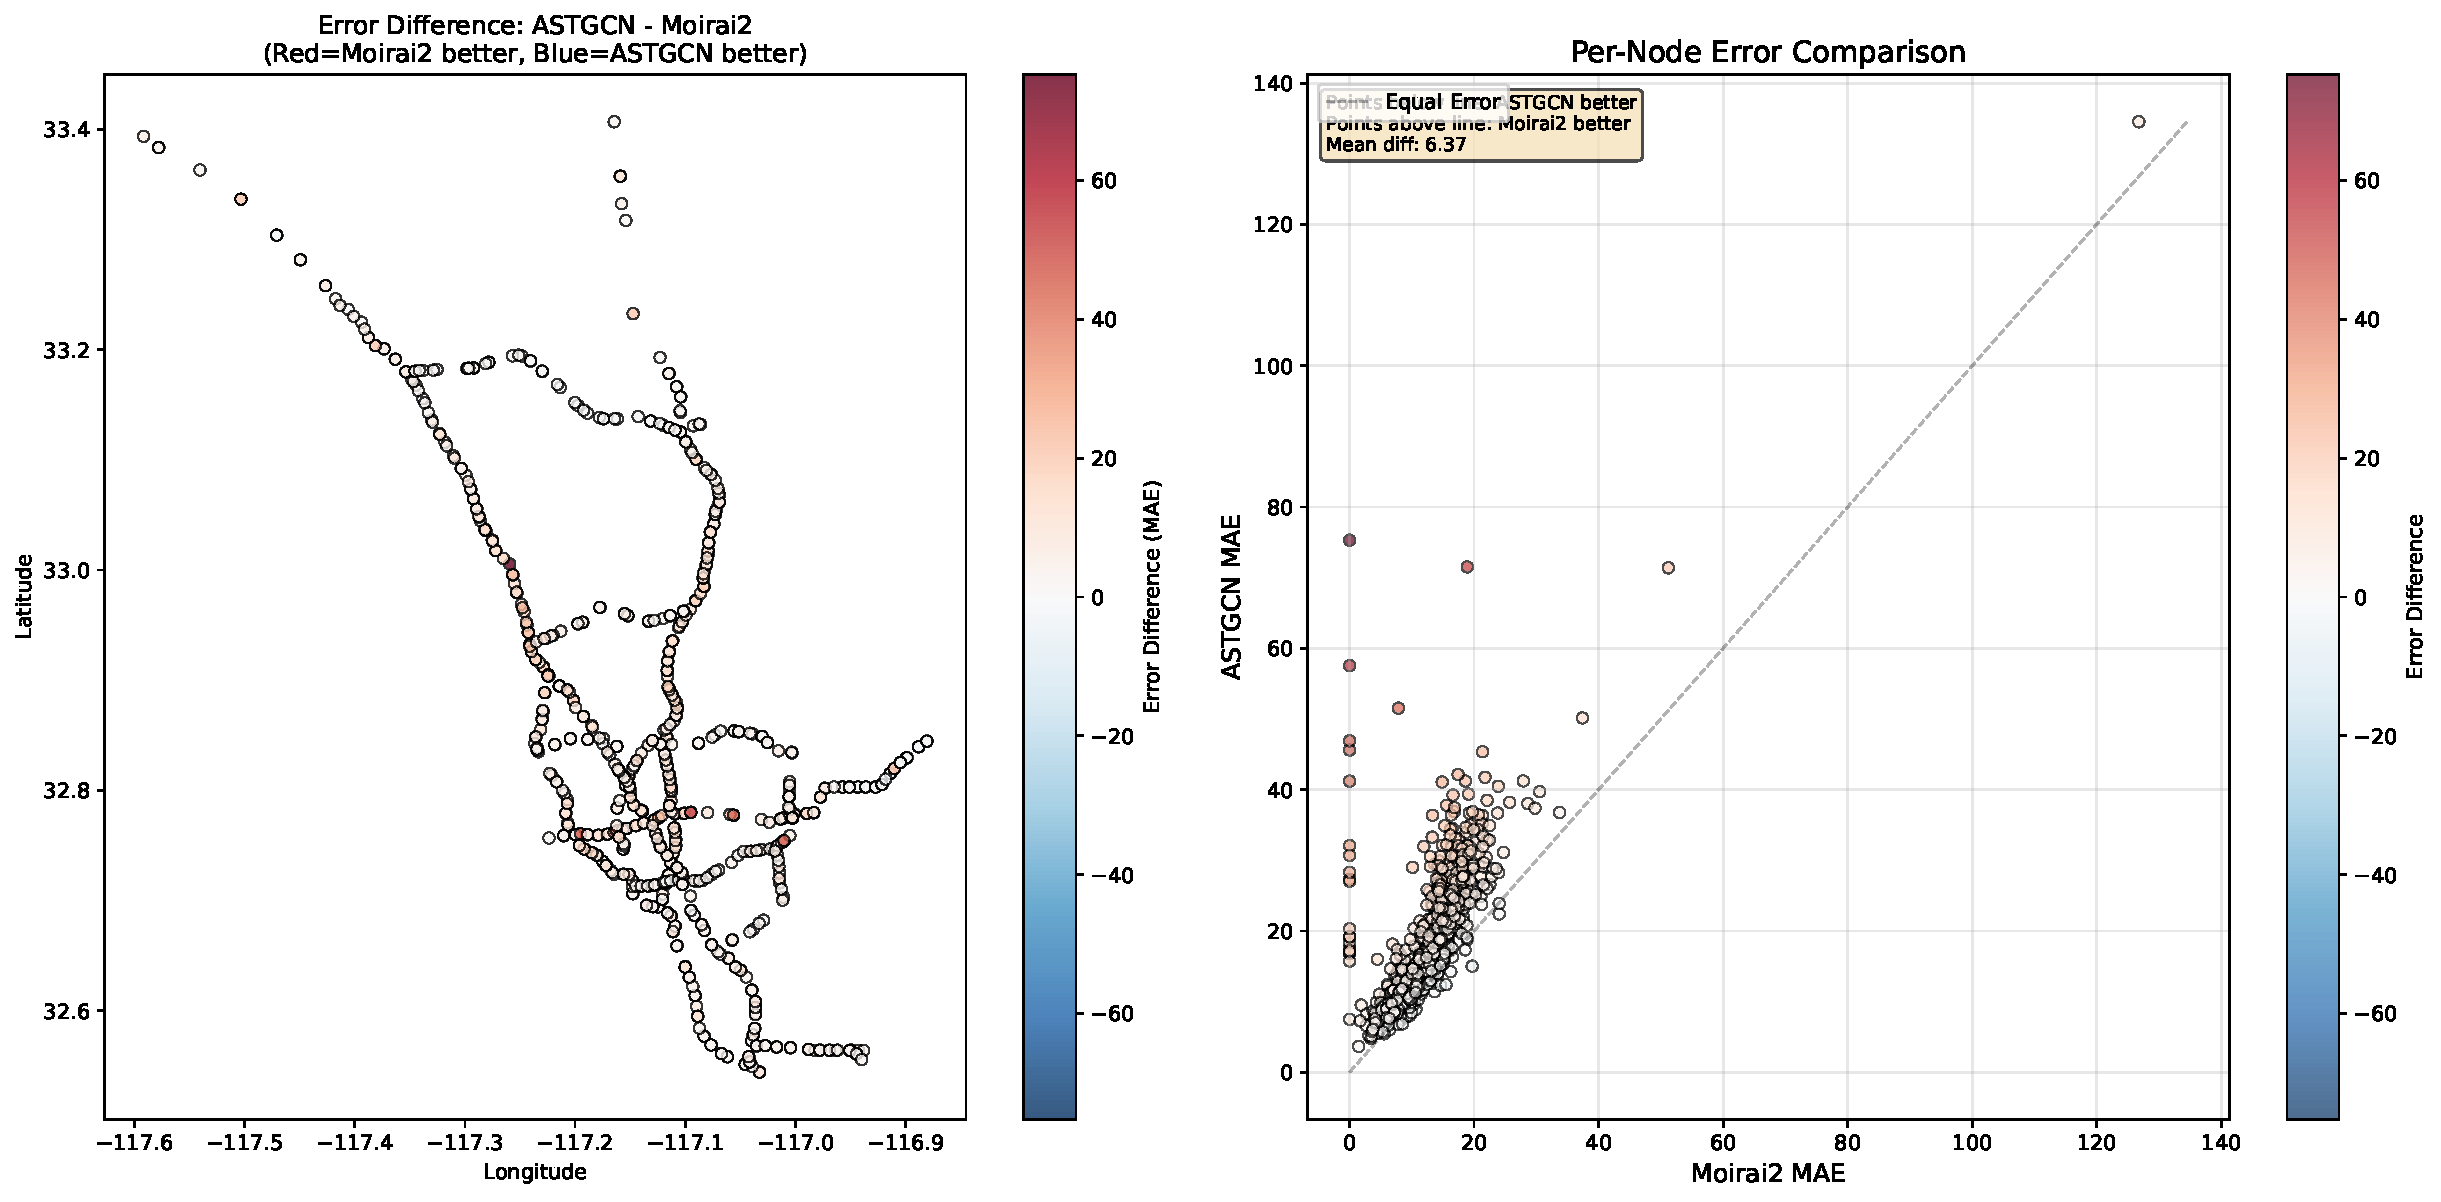
\includegraphics[width=1\linewidth]{images/moirai2_vs_astgcn.pdf}
    \caption{\textbf{Per-node error heterogeneity between Moirai2 and ASTGCN.}
    Left: spatial distribution of MAE difference (ASTGCN$-$Moirai2); red indicates Moirai2 achieves lower error and blue indicates ASTGCN achieves lower error.
    Right: per-node scatter of Moirai2 MAE vs.\ ASTGCN MAE; points above the diagonal favor Moirai2, and points below favor ASTGCN (mean MAE difference: 6.37).}
    \label{fig:moirai2_vs_astgcn}
\end{figure*}

\section{Detailed Analysis on SD dataset}


\subsection{Autocorrelation analysis on SD sensors}
To characterize the intrinsic temporal structure of SD traffic series, we analyze autocorrelation functions (ACF)
under three granularities: daily means (weekly-scale), hourly means (diurnal-scale), and the native sampling
(short-lag dynamics). Together, these views reveal a consistent multi-timescale pattern that informs context-length
selection and helps explain why different model classes excel under different horizons.

\begin{figure*}[t]
    \centering
    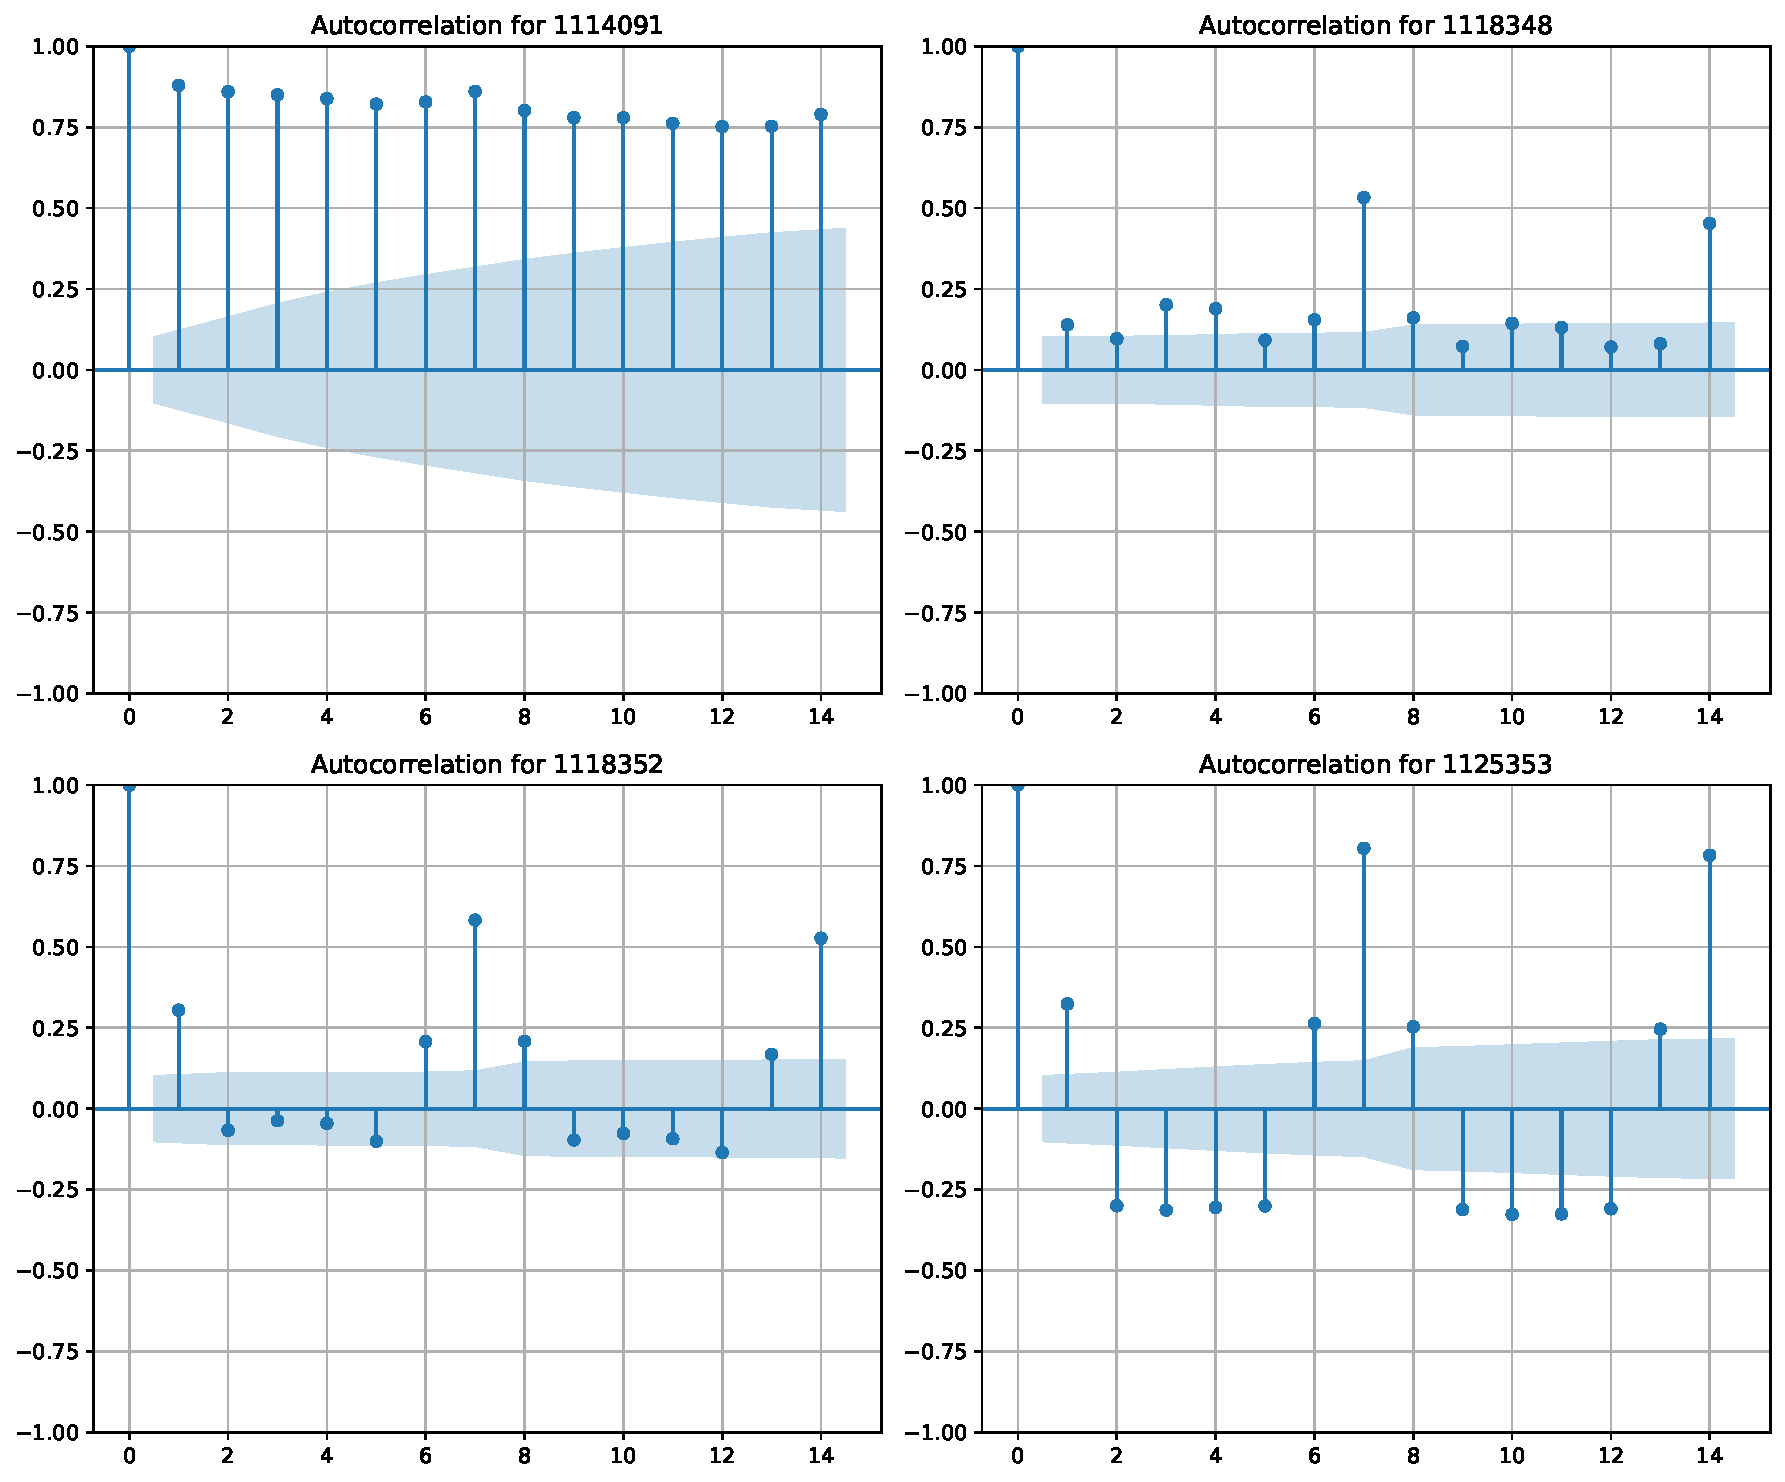
\includegraphics[width=1\linewidth]{images/auto/autocorrelation_plots.pdf}
    \caption{\textbf{Daily ACF on SD sensors (14 lags).} ACF of daily-averaged flow (1D resample, forward-filled),
    highlighting slow-varying structure and potential weekly recurrence (lags near 7 and 14 days). Shaded bands
    indicate 95\% confidence intervals.}
    \label{fig:acf_sd_daily}
\end{figure*}

\begin{figure*}[t]
    \centering
    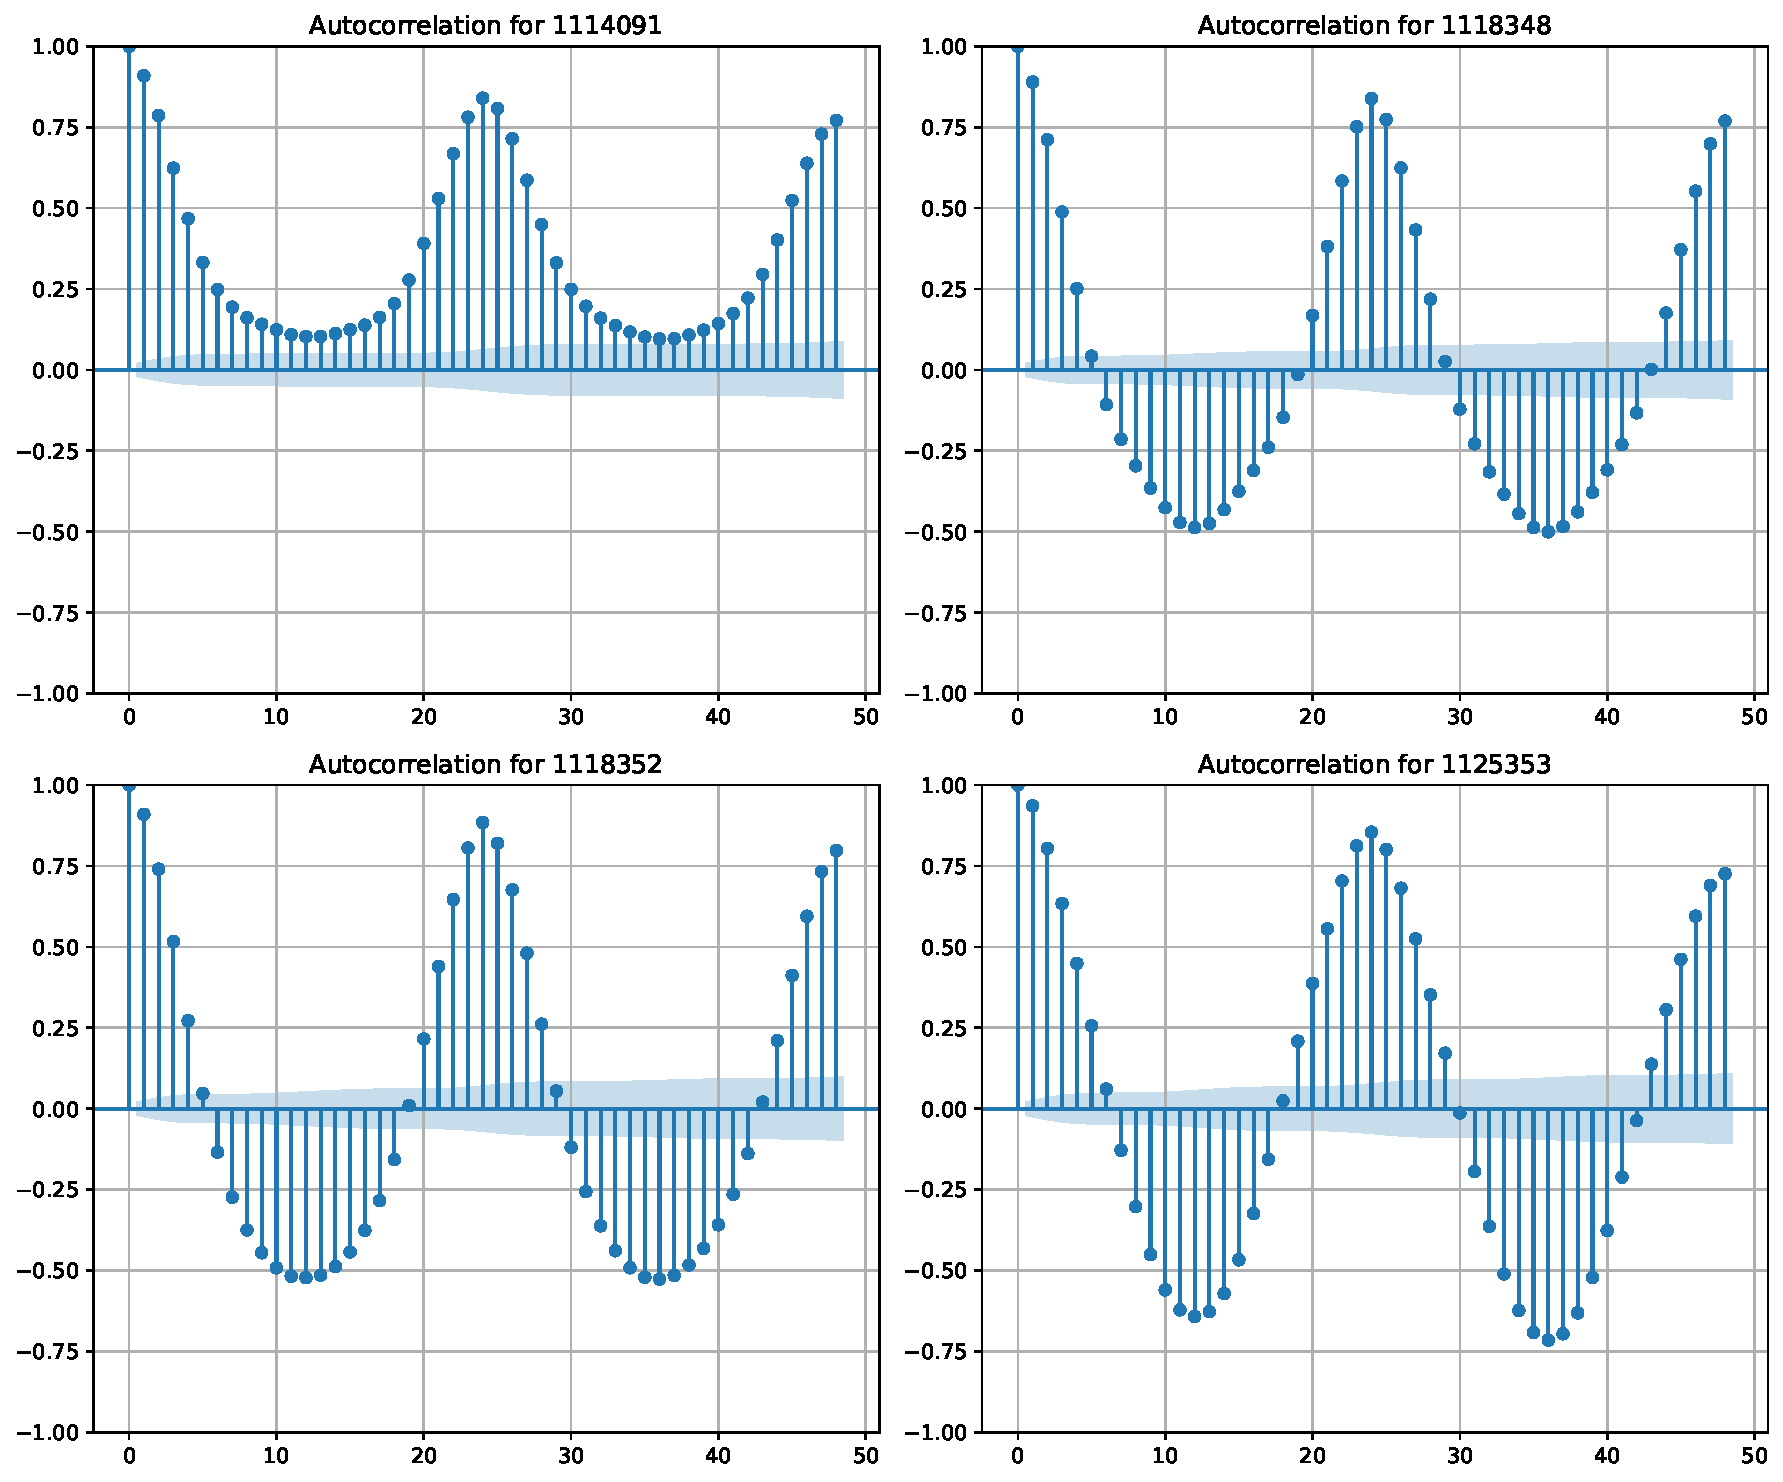
\includegraphics[width=1\linewidth]{images/auto/autocorrelation_plots_hourly.pdf}
    \caption{\textbf{Hourly ACF on SD sensors (48 lags).} ACF of hourly-averaged flow (1H resample, forward-filled).
    Clear periodicity emerges at daily-scale offsets (around 24 and 48 hours), reflecting diurnal commuting cycles
    that become exploitable once a full-day context is available. Shaded bands indicate 95\% confidence intervals.}
    \label{fig:acf_sd_hourly}
\end{figure*}

\begin{figure*}[t]
    \centering
    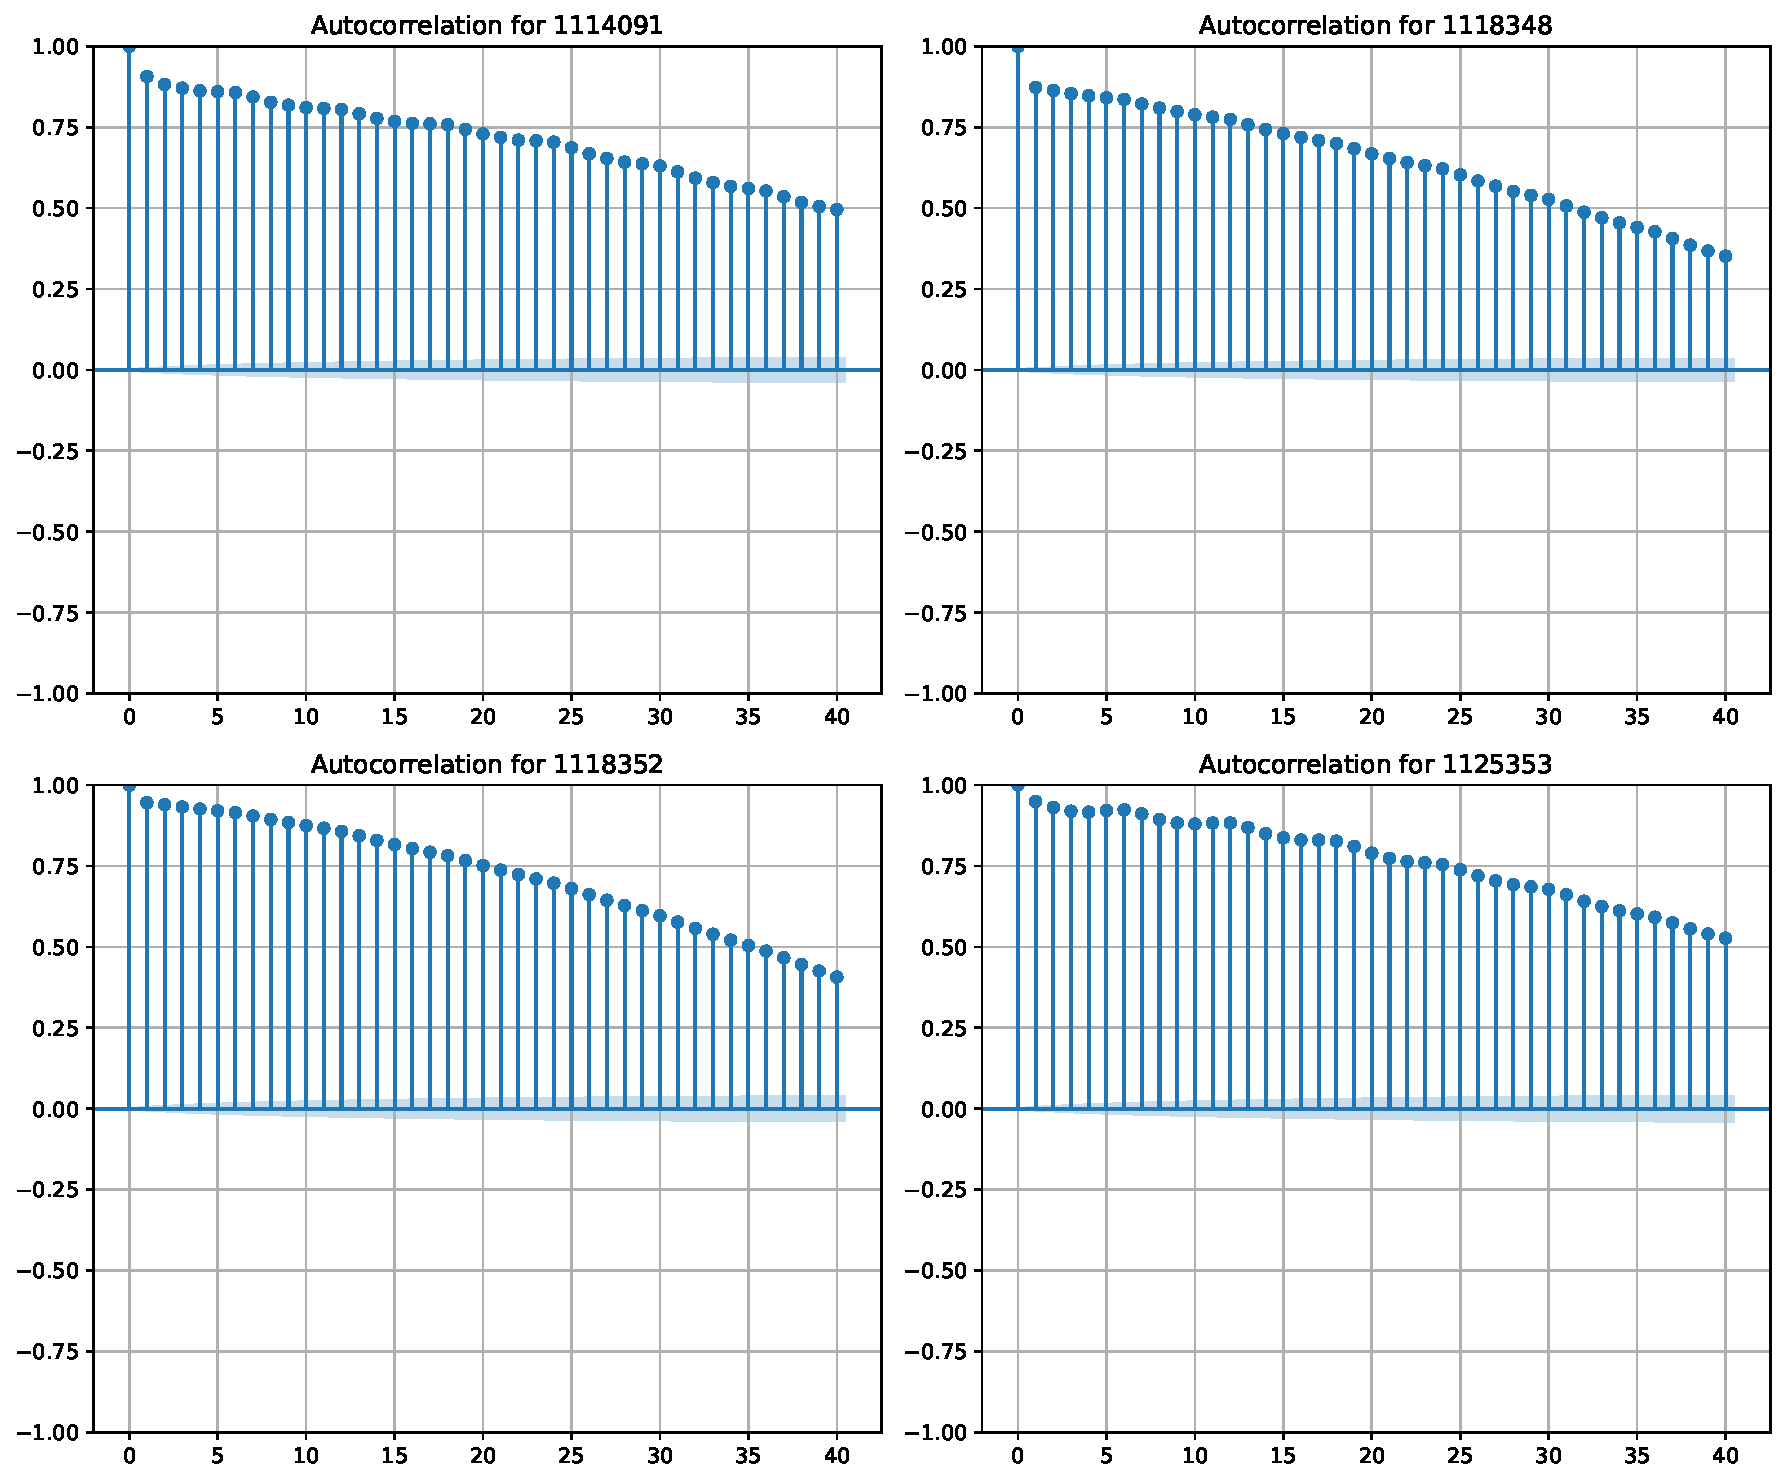
\includegraphics[width=1\linewidth]{images/auto/autocorrelation_plots_no_resample.pdf}
    \caption{\textbf{Native-resolution ACF on SD sensors (40 lags).} ACF computed on the original series
    (forward-filled), showing strong short-lag persistence and gradual decay over several hours, consistent with
    high predictability for short-horizon forecasting from recent context. Shaded bands indicate 95\% confidence
    intervals.}
    \label{fig:acf_sd_native}
\end{figure*}

\paragraph{Key observations and implications.}
At the native resolution (Fig.~\ref{fig:acf_sd_native}), all sensors exhibit strong short-lag dependence with a
slow decay, indicating that recent history alone carries substantial predictive signal—supporting why myopic or
``recent-driven'' models can remain competitive at very short horizons. After hourly aggregation
(Fig.~\ref{fig:acf_sd_hourly}), the ACF becomes strongly periodic, with pronounced re-correlation at 24--48 lags,
suggesting that providing a full diurnal context (e.g., 24 hours) should improve stability for medium horizons by
anchoring forecasts to daily structure. Finally, the daily ACF (Fig.~\ref{fig:acf_sd_daily}) shows longer-range
dependencies and, for some sensors, a weekly recurrence signal, motivating evaluation across multiple context
lengths rather than fixing a single $L$ for all methods and locations.


%\subsection{}
\subsection{Month-conditioned diurnal patterns on SD sensors}
\begin{figure*}[t]
    \centering
    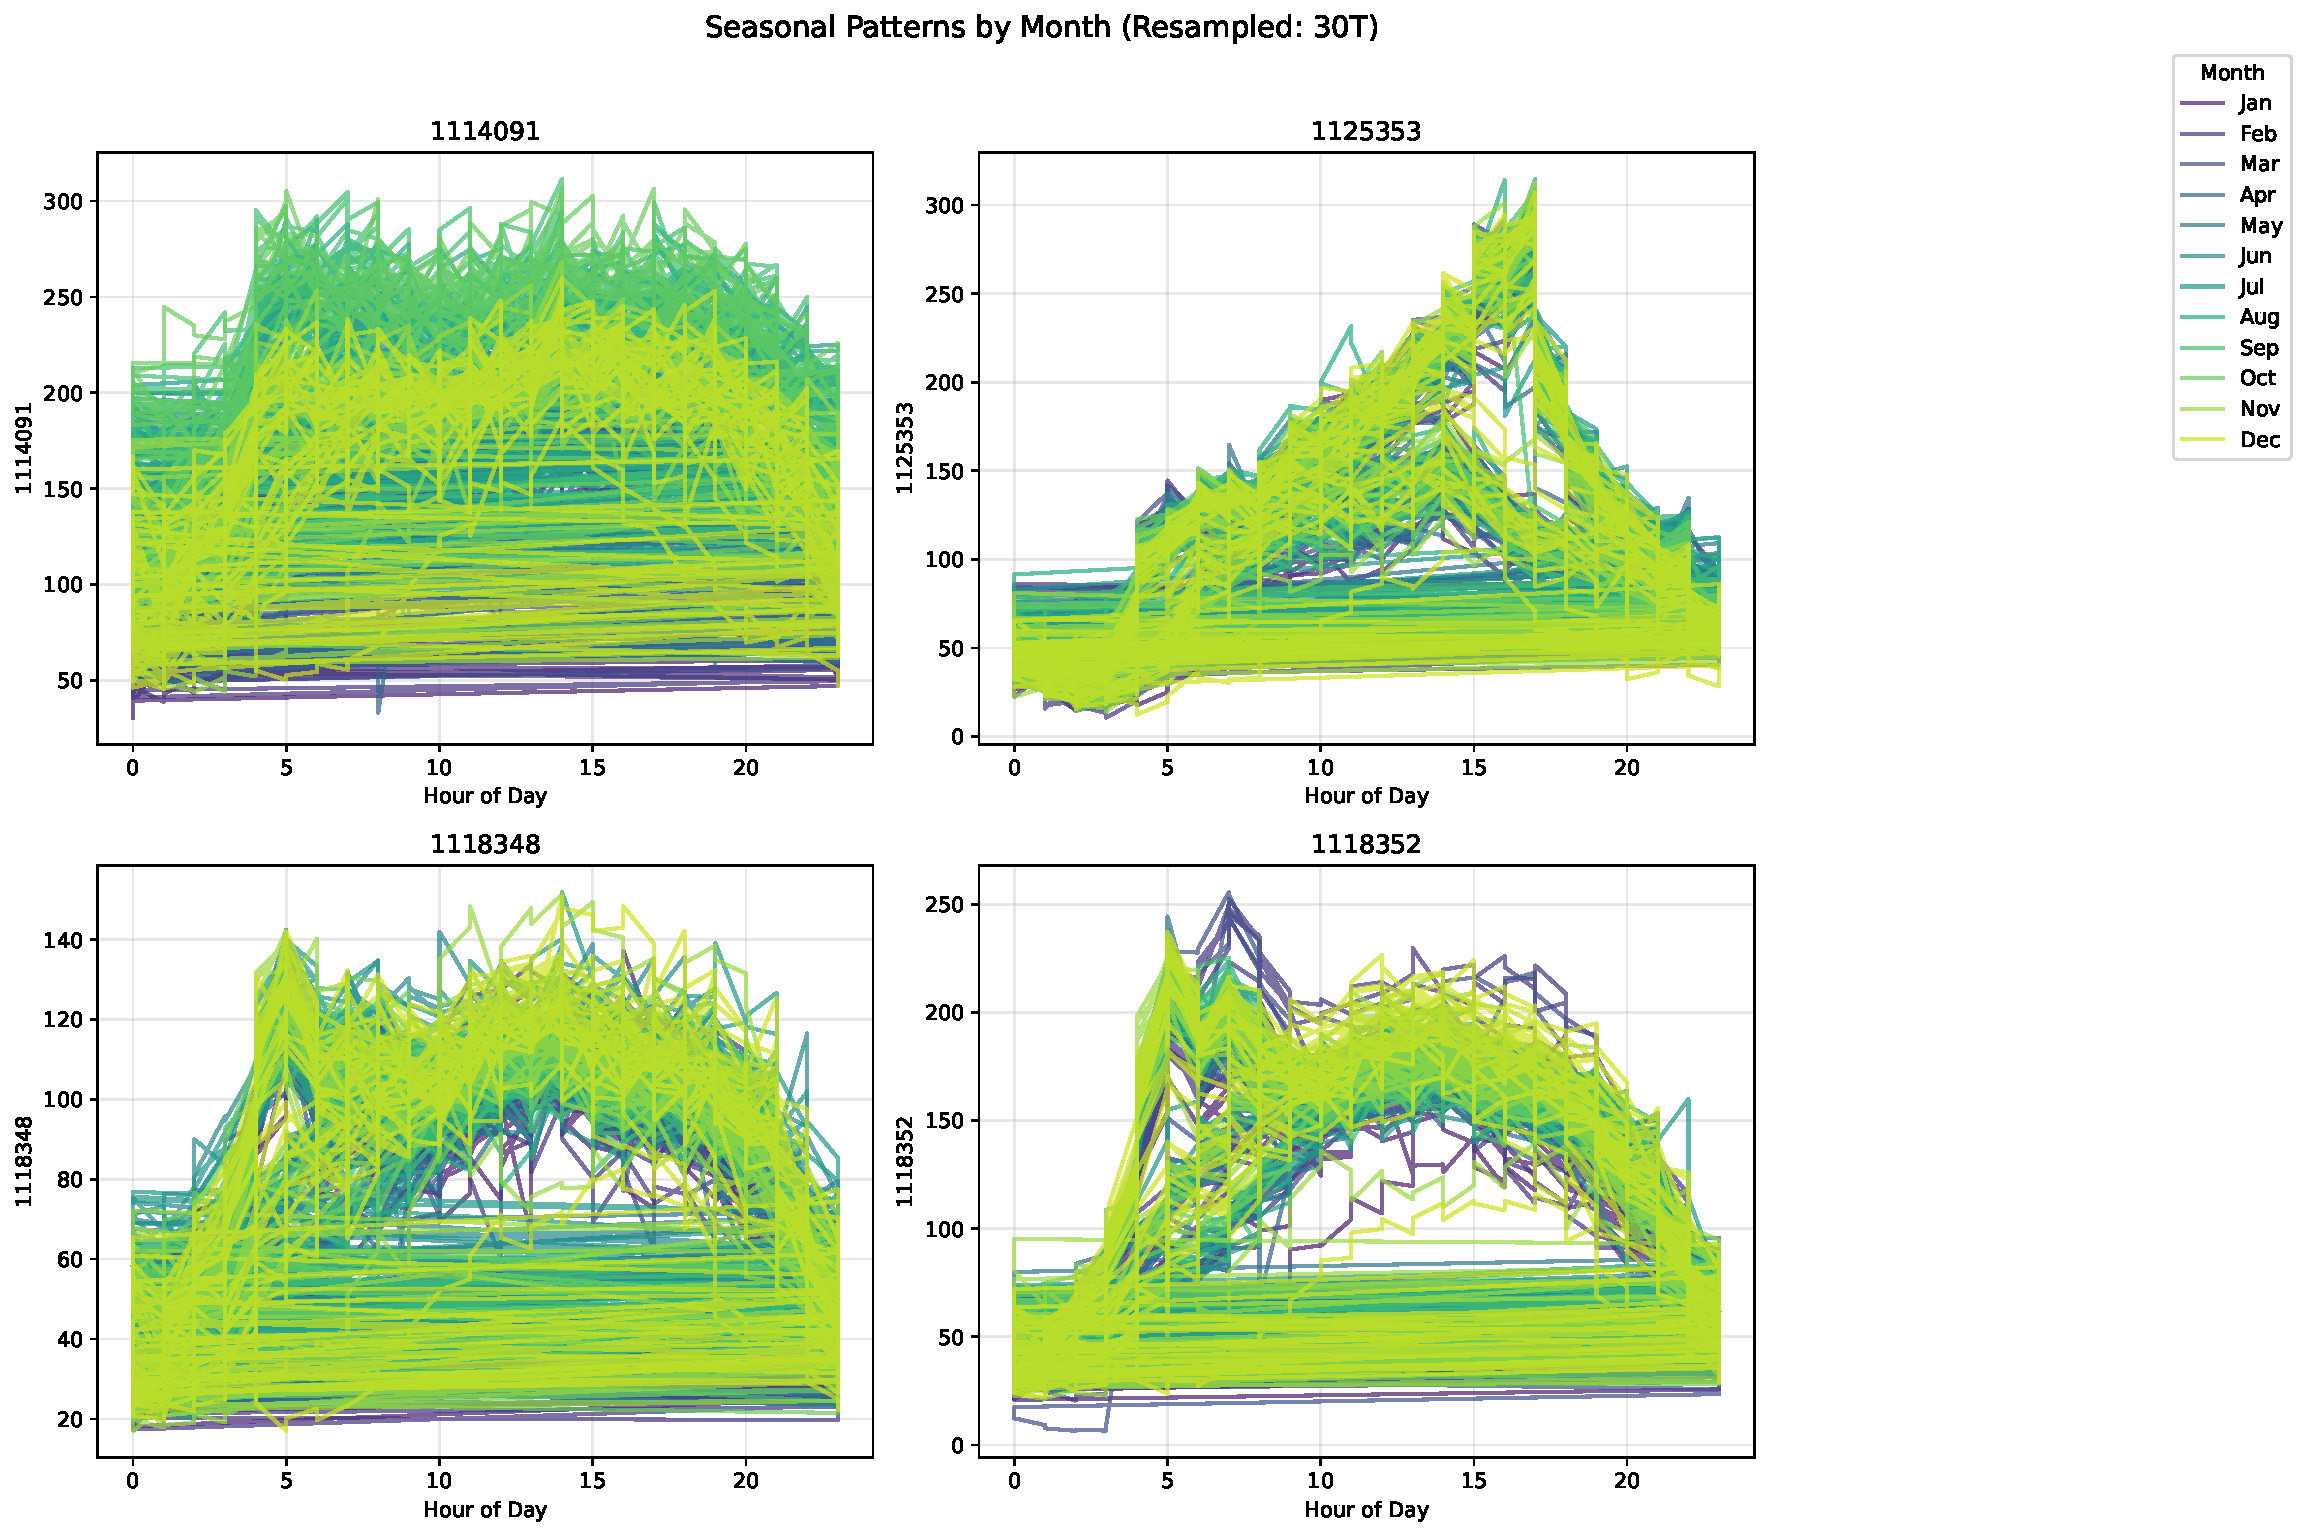
\includegraphics[width=\linewidth]{images/auto/seasonal_trends_with_legends.pdf}
    \caption{Month-conditioned diurnal profiles on SD sensors (30-min resample).}
    
    \label{fig:sd_month_diurnal}
\end{figure*}

For four representative SD sensors, we plot average flow versus hour-of-day after resampling to 30-minute bins in Figure~\ref{fig:sd_month_diurnal},
    with separate curves for each calendar month. Across all sensors, the dominant structure is diurnal: flow
    ramps up in the early morning (around 05:00), remains elevated through daytime, and decays into the night,
    indicating strong daily periodicity that can be exploited once a full-day context is available. Meanwhile,
    sensors exhibit clear heterogeneity in peak shape and amplitude (e.g., long daytime plateaus vs.\ sharper
    midday peaks), consistent with differences between mainline and more commuter- or locality-driven segments.
    The large within-month dispersion further suggests substantial day-to-day variability even after resampling,
    motivating models that combine diurnal anchoring with robustness to irregular disturbances (incidents, weather,
    special events).

\subsection{Forecasting Analysis}
The Moirai2–ASTGCN in Figure~\ref{fig:moirai2_vs_astgcn} comparison reveals strong node-level heterogeneity that is hidden by aggregate scores. Overall, the scatter plot shows that many sensors lie above the diagonal (with a positive mean MAE difference of ASTGCN$-$Moirai2), indicating that the transformer foundation model often achieves lower error. However, the spatial map shows this advantage concentrates on the most complex, high-variability corridors—e.g., dense freeway segments and weaving regions—where rapid regime changes and non-linear temporal patterns dominate, and a recent-driven transformer can track evolving dynamics effectively. In contrast, ASTGCN wins on a meaningful subset of sensors (points below the diagonal; blue regions), which plausibly correspond to branch roads, ramps, or low-flow locations where the local series is sparse/noisy and strongly influenced by nearby traffic states. In these “weak-signal” settings, explicit spatial coupling helps by borrowing information from correlated neighbors, yielding more stable forecasts. Taken together, the figure supports a practical takeaway: transformers can be preferable on highly dynamic, complex segments, while spatially aware models are advantageous on secondary links where inter-sensor dependence is a primary source of predictability.


% ---------------------------------------------------------------------------
% Preliminary appendix: full method x region x year grid.
% Place after Appendix D. Needs only multirow / pifont / graphicx (already in
% the preamble). Tables are generated -- do not hand-edit appendix_tables.tex:
%   python scripts/analysis/make_appendix_tables.py --out paper/appendix_tables.tex
% ---------------------------------------------------------------------------

\section{Extended Results: 33 Methods $\times$ 4 Regions $\times$ 2 Years}
\label{app:extended}

The main text reports year 2019 for a subset of the evaluated methods. This
appendix reports the complete re-run grid: all 33 methods in
Table~\ref{tab:app_coverage}, on all four LargeST subsets, for both 2018 and
2019. Beyond breadth it does three things the single-year tables cannot.
First, it adds two model families absent from the main text---deep state-space
models and linear forecasters---which turn out to occupy the gap between the
task-trained graph models and the pretrained forecasters. Second, the second
year converts the comparison into a replication: an ordering that survives both
years is a property of the method, whereas one that flips is a property of the
year. Third, it records which methods could not be run at all at scale, which
is itself a deployment result.

\subsection{Additional methods}
\label{app:extended:methods}

\textit{Deep state-space models (SSM).} Structured state-space sequence models
are task-trained, like the GNNs, but run per sensor series, like the foundation
models. That combination makes them the control this benchmark was missing: they
separate the contribution of the architecture class from the contribution of
large-scale pretraining, and they do so without a road graph. We evaluate a
minimal diagonal linear time-invariant model (\textbf{Linear SSM}),
\textbf{S4}~\citep{gu2022s4, gu2022s4d} with HiPPO-inspired initialization and a
learnable step size, the \textbf{LRU}~\citep{orvieto2023lru} with complex
eigenvalues and an output gate, and \textbf{Mamba-v2}~\citep{dao2024mamba2}, a
selective SSM with an input-dependent state transition. Each maps a length-$L$ univariate context to $H$ steps directly and
is trained under the same splits, normalization and early stopping as the GNNs.

\textit{Linear forecasters.} \textbf{DLinear} and \textbf{NLinear}~\citep{zeng2023transformers}
are single-layer linear maps from context to horizon---the former over a
trend/seasonal decomposition, the latter over a last-value-normalized input.
They were introduced as evidence that much of the reported gain from deep
forecasters is recoverable linearly, and as the cheapest trained methods here
they calibrate what the rest of the table buys.

\subsection{Coverage and failures at scale}
\label{app:extended:coverage}

Table~\ref{tab:app_coverage} records which methods ran on which subset. The
gaps are not incidental and they fall on one family: the $O(N^2)$ graph
operators exhaust GPU memory as the sensor count grows, so \textbf{STGODE} is
unavailable on every subset, \textbf{D2STGNN} beyond SD, and \textbf{DGCRN}
beyond SD and GBA~2018. These methods are kept as rows in every table, with
their entries shown as ``-'', so that the composition of each family stays
visible. This matters for reading the tables, because the
unavailable models are not arbitrary members of their family: \texttt{DGCRN}
records the lowest Avg MAE of any graph model on SD in both years (17.65 in 2019,
17.13 in 2018) and \texttt{D2STGNN} places third or fourth, yet neither can be
run on GLA or CA. The graph family's strongest member is therefore absent from
exactly the subsets where the forecasting problem is hardest, and the GLA and CA
columns compare the remainder. A missing cell means the run did not produce a usable result---never
that the method scored poorly.


\subsection{Results by region and year}
\label{app:extended:tables}

Tables~\ref{tab:app_sd_2019}--\ref{tab:app_ca_2018} give the grid, one table per
subset and year, in the column layout of the main text. Best per column is bold,
runner-up underlined; comparisons are within a table, never across them. A
``-'' marks a method that did not produce a usable result on that subset, not a
poor score.

FlowState is listed for completeness and is unavailable throughout. We discuss
each subset over both years in turn, then draw the comparison across regions.

\subsubsection{San Diego (716 sensors)}
\label{app:extended:sd}

SD is the smallest subset and the only one where the graph family is
competitive. \texttt{DGCRN} is the best graph model in both years (Avg MAE
17.13 in 2018, 17.65 in 2019) and in 2019 it beats every state-space model
(\texttt{LRU}, 18.41); in 2018 the order reverses by a small margin
(\texttt{LRU} 16.97 against \texttt{DGCRN} 17.13). At the shortest horizon the
gap to the pretrained models is narrow---\texttt{DGCRN} reaches 14.58 MAE at
$H{=}3$ in 2018 against \texttt{Sundial}'s 14.24---so on a network of this size
the spatial prior is close to paying for itself. It does not hold up as the
horizon extends: \texttt{DGCRN} degrades by a factor of $1.43$ from $H{=}3$ to
$H{=}12$ while \texttt{Sundial} is flat, and the full-grid ordering by Avg MAE
is \texttt{Sundial} $<$ \texttt{Moirai-2} $<$ \texttt{Chronos-Bolt} $<$
\texttt{Kairos} before any task-trained model appears.

\begin{insightbox}
\textit{Takeaway:} On the smallest network the graph models are genuinely
competitive at short horizons and the best of them is level with the best
state-space model, but they are already behind every pretrained model, and
their advantage is confined to $H{=}3$.
\end{insightbox}

\subsubsection{Bay Area (2,352 sensors)}
\label{app:extended:gba}

At three times SD's size the picture changes. The best graph model drops to
\texttt{DSTAGNN} (21.09) in 2018 and \texttt{AGCRN} (21.21) in 2019, while the
best state-space model (\texttt{Mamba-v2}, 19.43 and 19.30) leads it by $7.9\%$
and $9.0\%$ respectively. \texttt{D2STGNN} is unavailable on this subset and
\texttt{DGCRN} on 2019, so the family is evaluated without two of its three best
SD members. In 2019 even the linear forecasters overtake the graph family
(\texttt{DLinear} 19.90 against \texttt{AGCRN} 21.21), which is notable because
a single linear layer over a univariate context carries no spatial information
whatsoever. The top four places again go to the same four pretrained models, led
by \texttt{Sundial} (16.74 and 16.15); \texttt{TimesFM} is not among them and
trails the best state-space model in both years.

\begin{insightbox}
\textit{Takeaway:} At 2,352 sensors the graph family has already fallen behind
the state-space models, and in 2019 behind a single linear layer---the first
subset where spatial message passing returns nothing measurable.
\end{insightbox}

\subsubsection{Greater Los Angeles (3,834 sensors)}
\label{app:extended:gla}

GLA repeats the GBA pattern with a wider margin and more attrition:
\texttt{D2STGNN}, \texttt{DGCRN} and \texttt{STGODE} are all unavailable, and
\texttt{AGCRN} is the best remaining graph model in both years (19.55, 22.49).
The best state-space model leads it by $6.3\%$ in 2018 (\texttt{Mamba-v2},
18.32) and by $19.4\%$ in 2019 (\texttt{S4}, 18.13). The linear family is
roughly level with the graph family here---\texttt{NLinear} 18.86 against
\texttt{AGCRN} 19.55 in 2018, and 22.71 against 22.49 in 2019---and is the most
horizon-stable non-pretrained family on this subset, with an $H{=}12$ to
$H{=}3$ ratio of $1.13$--$1.20$ against $1.48$--$1.66$ for the graph models.
\texttt{Sundial} leads overall in both years (15.29, 15.85).

\begin{insightbox}
\textit{Takeaway:} On GLA the state-space models lead the graph family by up to
$19.4\%$, and two linear layers are statistically indistinguishable from the
best graph model while degrading far more slowly with horizon.
\end{insightbox}

\subsubsection{California (8,600 sensors)}
\label{app:extended:ca}

CA is the largest subset, the most punishing for the graph family---which loses
three members to memory---and the one subset where the two years disagree about
which family the graph models fall below. In 2018 their best survivor,
\texttt{GWNET} (22.29), is beaten not only by the state-space models
(\texttt{LRU} 17.24) and the linear forecasters (\texttt{DLinear} 17.79) but by
the \emph{ensembles of classical regressors} (\texttt{weighted} 21.70): a
weighted average of seasonal-naive, ridge, linear regression and random forest,
none of which sees more than one sensor's history. In 2019 that last comparison
reverses, and by a wide margin---the best graph model (\texttt{AGCRN}, 21.31)
beats every ensemble (best 31.62). The reversal is a property of the ensembles
rather than of the graph models: their own inputs degrade sharply between the
two years (\texttt{ridge} 24.11 to 38.33, \texttt{seasonal\_naive} 34.85 to
45.56), and the ensembles inherit that. What does replicate is the deficit to
the graph-free \emph{trained} models, which is the largest on any subset: the
best state-space model leads the best graph model by $29.3\%$ in 2018 and
$19.3\%$ in 2019. The graph family also records its worst horizon degradation
here ($1.97$ in 2018 from $H{=}3$ to $H{=}12$, against $1.21$ for the linear
models). \texttt{Sundial} leads in both years (14.29, 14.73).

\begin{insightbox}
\textit{Takeaway:} At 8,600 sensors the graph family trails the state-space
models by $19$--$29\%$ in both years, its largest deficit anywhere. Where it
sits relative to the \emph{classical ensembles} does not replicate---below them
in 2018, well above them in 2019---and that swing is driven by the ensembles'
inputs, not by the graph models. Single-year orderings between adjacent families
should not be read as stable.
\end{insightbox}

\subsubsection{Across regions}
\label{app:extended:across}

\textit{Four pretrained models occupy the top of every table---but the family is
not uniform.} \texttt{Sundial}, \texttt{Moirai-2}, \texttt{Chronos-Bolt} and
\texttt{Kairos} take the first four places by Avg MAE in all eight cells,
without exception, and their internal ordering is fixed throughout, with only
the third and fourth places exchanging. \texttt{Sundial} is first in every cell
not only on Avg MAE but also at $H{=}3$ and at $H{=}12$ individually---so the
main text's split verdict, that graph models own the short horizon while
pretrained models own the long one, does not survive the wider grid.

The other two pretrained models are the counterexample. \texttt{TimesFM} places
9th to 14th overall and is beaten by the best state-space model in every one of
the eight cells, by the best graph model in four of them, and by a single
linear layer in four; \texttt{Moirai-Small} is $2.0$--$2.6\times$ worse
than \texttt{Sundial} everywhere and behind every task-trained model. Neither
pretraining nor parameter count is therefore sufficient on its own:
\texttt{TimesFM} is roughly four times the size of \texttt{Sundial} and
uniformly worse. The spread \emph{inside} the pretrained family---13.83 to 31.54
Avg MAE on SD~2018---exceeds the spread between families, so ``foundation
model'' is not a useful unit of comparison.

\textit{The graph family's standing falls monotonically with network size.}
Read across the four subsets, the gap between the best graph model and the best
state-space model widens in one direction, and both years agree at every step:
level on SD (716 sensors; the graph model is $0.9\%$ behind in 2018 and $4.1\%$
ahead in 2019), $8$--$10\%$ behind on GBA (2,352), $7$--$24\%$ behind on GLA
(3,834) and $19$--$29\%$ behind on CA (8,600). This is the clearest single
pattern in the grid, and it runs opposite to the intuition that spatial coupling
should matter more as the network grows. We return to it in Section~\ref{app:extended:asymmetry}.

\textit{Horizon stability separates the families cleanly.} Taking the $H{=}12$
to $H{=}3$ MAE ratio of each family's best member, foundation models degrade
least ($0.97$--$1.33$), then SSMs ($1.22$--$1.52$), then graph models
($1.36$--$1.97$), then ensembles and single ML regressors ($1.5$--$2.4$). The
graph models' worst degradation is on CA ($1.97$), the subset where they are
already weakest, so the accuracy gap and the stability gap compound rather than
offset.

\textit{On SD~2018 the foundation models invert the horizon curve.} The ratio
falls below one for three of the six foundation models on MAE
(\texttt{Chronos-Bolt} $0.93$, \texttt{Moirai-2} $0.95$, \texttt{Sundial}
$0.97$) and for four of the six on RMSE ($0.94$--$0.99$): the three-hour
forecast is more accurate than the 45-minute one. The two exceptions are the two
weakest models here, \texttt{TimesFM} ($1.62$) and \texttt{Moirai-Small}
($1.98$), so the inversion tracks forecast quality rather than pretraining as
such. That RMSE falls too argues
against a hedging artifact, since a model retreating toward a smooth
climatological mean would lower MAE but not RMSE; so does the fact that the only
non-pretrained method anywhere in the grid with a ratio below one is
\texttt{seasonal\_naive} ($0.99$), which is pure daily periodicity by
construction. The effect is confined to this subset---elsewhere every ratio
exceeds one---and we report the pattern without claiming its mechanism.

\textit{Classical baselines behave as expected, with one caveat for reading the
tables.} Ensembling is a cheap and reliable gain: all three ensembles beat the
best single regressor in all eight cells, though which ensemble wins is not
stable and should not be read as a finding. The MAPE columns for the lag-feature
regressors, however, grow much faster with horizon than their MAE columns do,
reaching $53\%$ at $H{=}12$ for \texttt{ridge} on GBA~2018. This reflects
iterative roll-out compounding on low-flow sensors, where small absolute errors
are large relative ones; MAE and RMSE are the more trustworthy columns for those
rows.

\subsection{The family ordering is not an artifact of subset choice}
\label{app:extended:stats}

Everything above is a point estimate on eight region-year cells, which invites
the obvious objection: that the ordering reflects which cells happened to finish
rather than a property of the methods. We test this with the standard protocol
for comparing methods over multiple datasets~\citep{demsar2006}---a Friedman test
on the per-cell ranks, then a post-hoc test on the pairwise differences---using
one representative per family, since the family ordering is the claim at issue.

Table~\ref{tab:app_ranks} gives the average ranks. The Friedman test rejects the
null hypothesis that the seven representatives are equivalent
($\chi^2 = 46.1$, $p = 2.8\times10^{-8}$, $k=7$, $N=8$), as it does for the
wider set of all 29 methods that completed on every cell
($\chi^2 = 207.8$, $p < 10^{-28}$, $k=29$). \texttt{Sundial} attains an average
rank of exactly $1.00$: it is first in all eight cells, not first on average.

\begin{table}[t]
\centering
\caption{Average rank by Avg MAE across the eight region-year cells (lower is
better), one representative per family. Friedman $\chi^2 = 46.1$,
$p = 2.8\times10^{-8}$. Bonferroni--Dunn CD${}=2.85$ with \texttt{Sundial} as
control; Nemenyi CD${}=3.19$ for all pairs.}
\label{tab:app_ranks}
\begin{tabular}{l|l|c}
\toprule
Family & Representative & Avg.\ rank \\
\midrule
Foundation Models & \texttt{Sundial}   & 1.00 \\
SSM               & \texttt{Mamba-v2}  & 2.12 \\
Linear            & \texttt{NLinear}   & 3.25 \\
GNN-based         & \texttt{GWNET}     & 3.75 \\
Ensembles         & \texttt{median}    & 4.88 \\
ML Baselines      & \texttt{ridge}     & 6.00 \\
Simple Baselines  & \texttt{naive}     & 7.00 \\
\bottomrule
\end{tabular}
\end{table}

\textit{What the post-hoc test can and cannot resolve.} Taking \texttt{Sundial}
as the control and applying the Bonferroni--Dunn correction gives a critical
difference of $2.85$ ranks: it separates the pretrained representative from the
ensemble, ML and simple baselines, but---narrowly---still \emph{not} from the
graph representative, whose rank differs by $2.75$. Nemenyi's all-pairs
correction is more conservative still ($3.19$) and does not change that. The
binding constraint is the number of datasets rather than the size of the effect:
these omnibus procedures control the family-wise error rate over every pair
simultaneously, and eight cells is near the lower end of what they can resolve.

\textit{Pre-specified pairwise comparisons.} For the two contrasts this appendix
actually makes, a directly targeted paired test is more informative. Across the
eight cells \texttt{Sundial} beats the best graph model in each one (8/8,
Wilcoxon signed-rank $p = 0.0078$, mean margin $5.05$ MAE) and the best
state-space model in each one (8/8, $p = 0.0078$, margin $2.92$). The best
state-space model beats the best graph model in seven of eight cells
($p = 0.023$; the sign test alone, discarding magnitudes, gives $p = 0.070$).
Restricting to the three larger subsets, where
Section~\ref{app:extended:tables} locates the effect, the state-space models win
all six cells ($p = 0.031$), which with $N=6$ is the smallest two-sided $p$ the
test can return and is therefore significant at $\alpha = 0.05$ by the narrowest
possible margin.

The ordering therefore survives the objection at the level it is claimed---it is
stable across subsets, and the pretrained family separates significantly from
everything below the state-space models---while what eight datasets cannot
certify is the gap between families adjacent in the ranking.

\textit{Caveats.} Each cell contributes one number per method from a single
training run, so these tests treat run-to-run variance as zero and speak only to
consistency across region-years. They are not a substitute for repeated seeds,
which the compute budget did not allow across the full grid.

\begin{figure*}[t]
\centering
\begin{subfigure}[t]{0.32\linewidth}
  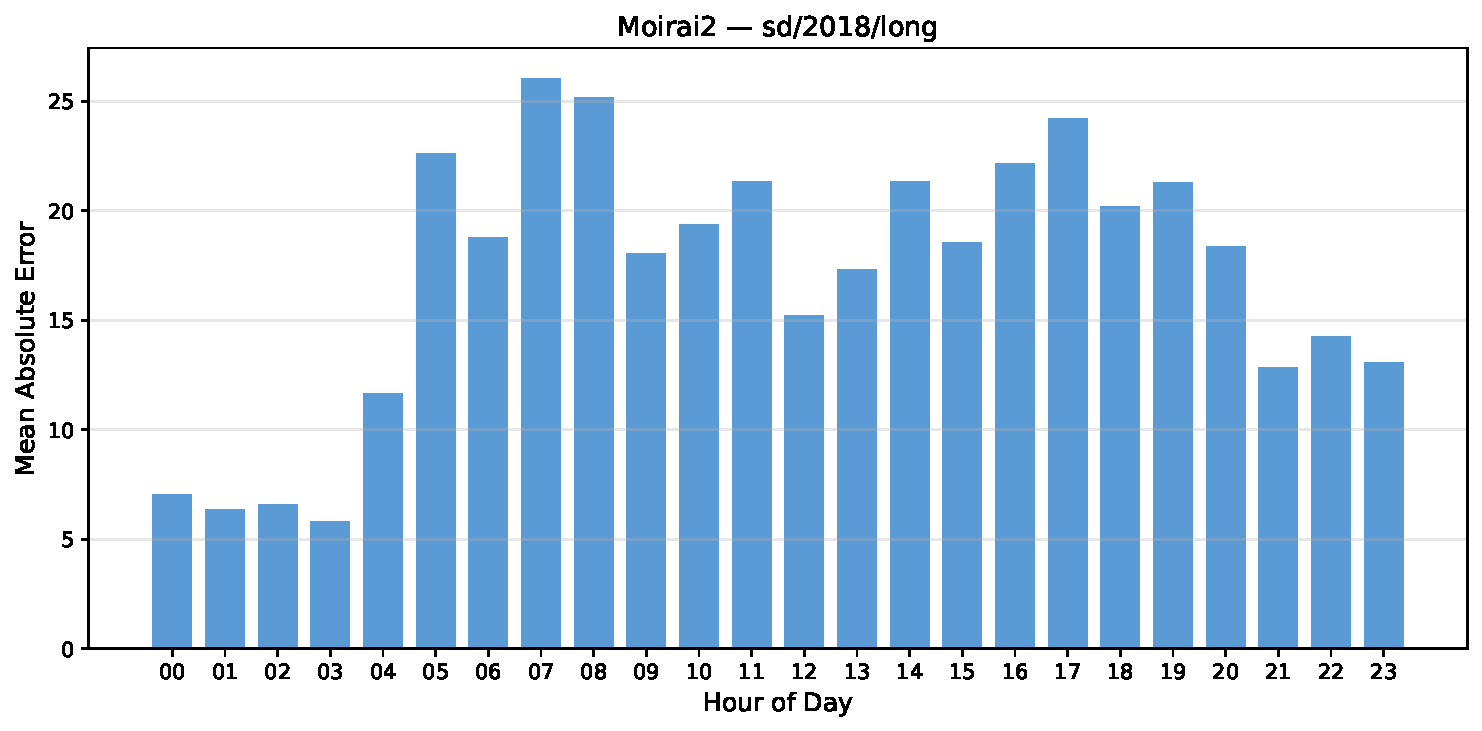
\includegraphics[width=\linewidth]{figs/hourly_mae_moirai2.pdf}
  \caption{\texttt{Moirai-2} (pretrained)}
\end{subfigure}
\hfill
\begin{subfigure}[t]{0.32\linewidth}
  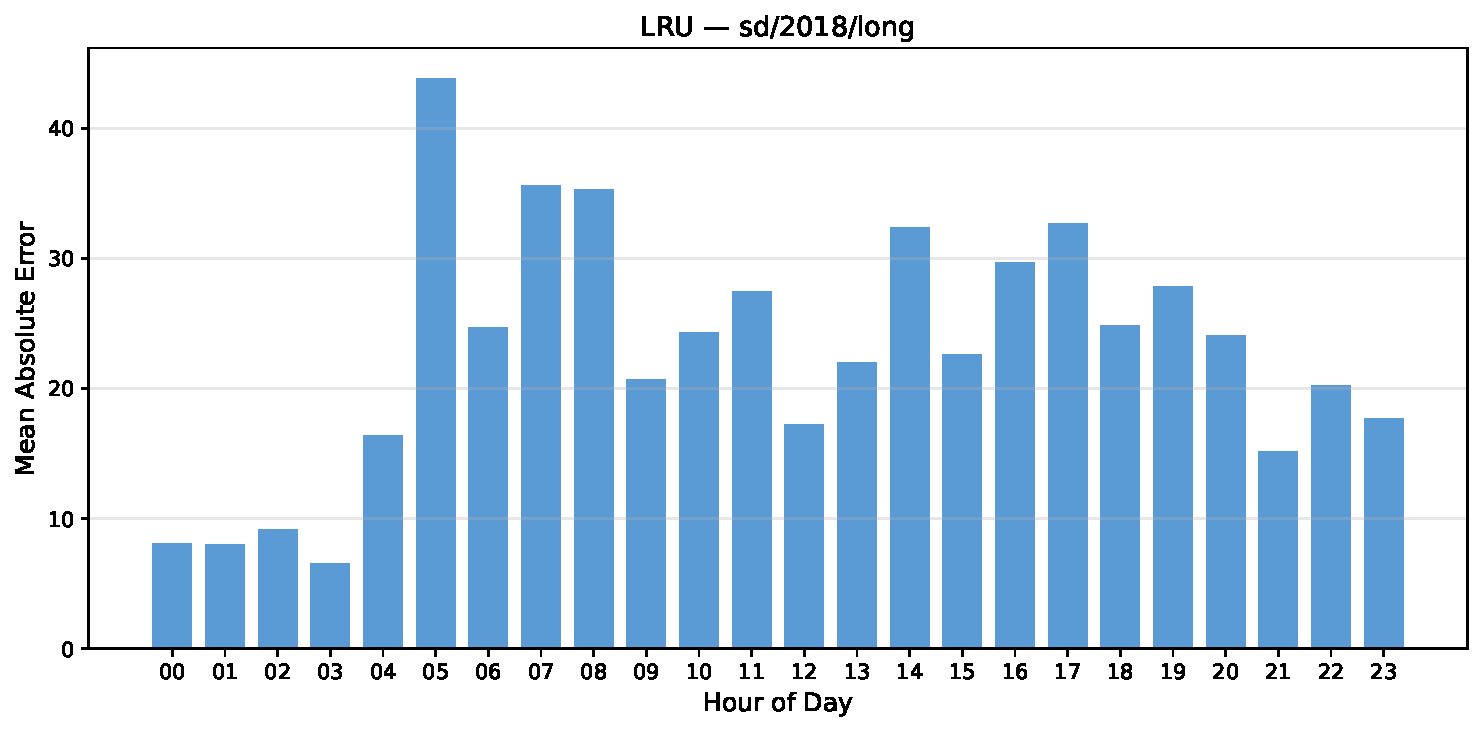
\includegraphics[width=\linewidth]{figs/hourly_mae_lru.pdf}
  \caption{\texttt{LRU} (state-space)}
\end{subfigure}
\hfill
\begin{subfigure}[t]{0.32\linewidth}
  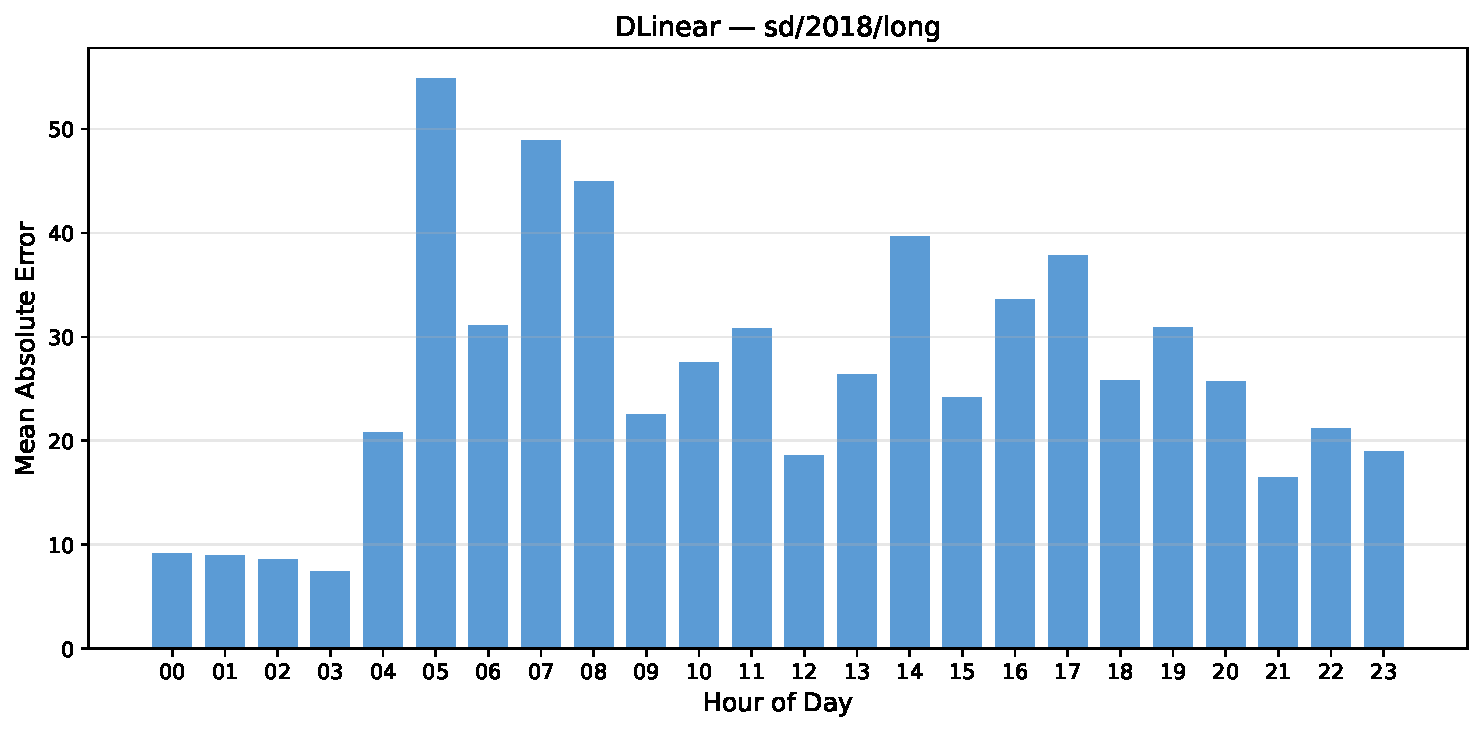
\includegraphics[width=\linewidth]{figs/hourly_mae_dlinear.pdf}
  \caption{\texttt{DLinear} (linear)}
\end{subfigure}
\\[4pt]
\begin{subfigure}[t]{0.32\linewidth}
  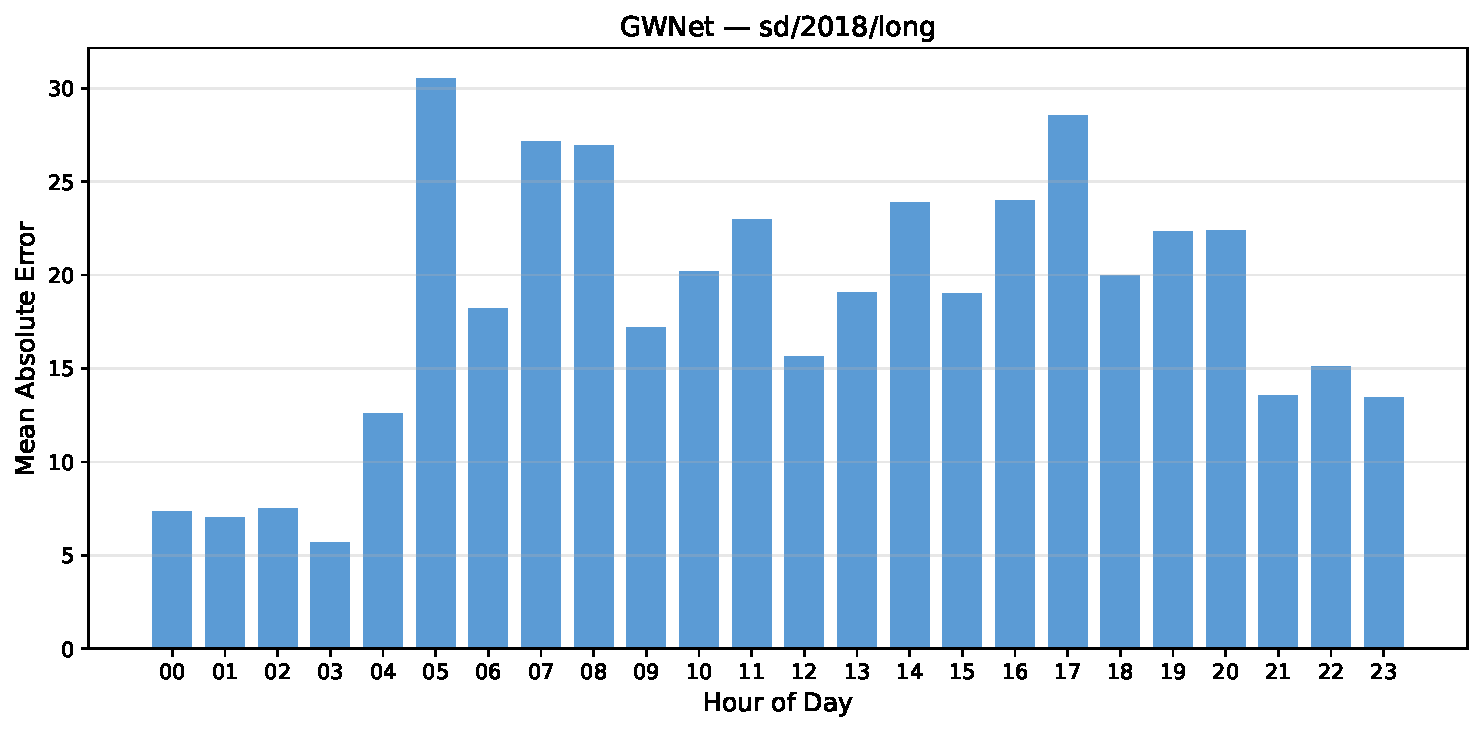
\includegraphics[width=\linewidth]{figs/hourly_mae_gwnet.pdf}
  \caption{\texttt{GWNET} (graph)}
\end{subfigure}
\hfill
\begin{subfigure}[t]{0.32\linewidth}
  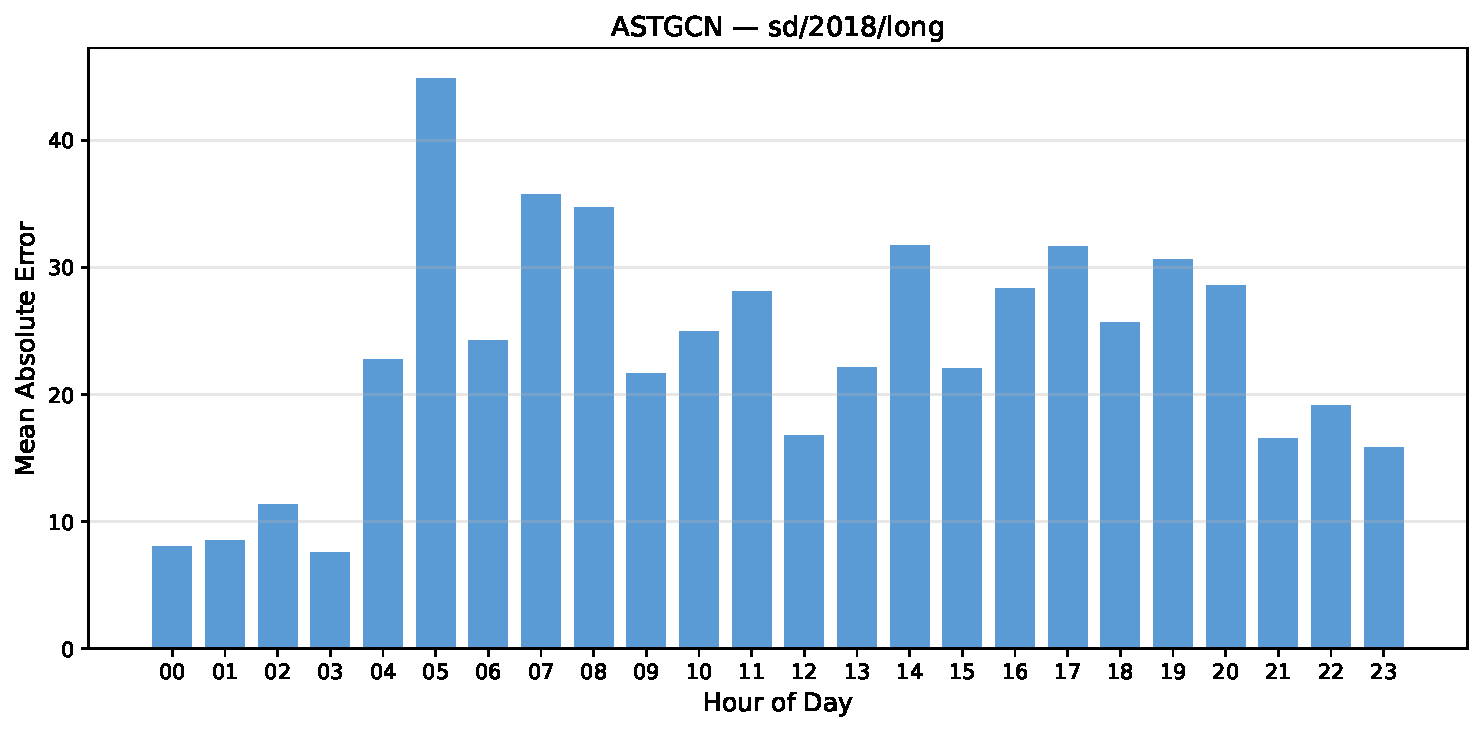
\includegraphics[width=\linewidth]{figs/hourly_mae_astgcn.pdf}
  \caption{\texttt{ASTGCN} (graph)}
\end{subfigure}
\hfill
\hspace{0.32\linewidth}
\caption{Hour-of-day MAE on SD~2018, averaged over all 716 sensors and the
twelve forecast steps, one representative per family. All five are scored on the
same 500 windows (2018-10-30 to 12-31), a wider span than the benchmark tables
so that every hour is sampled across two months; panels are comparable with each
other but not with the tables. All five bottom out at 03:00 and are hardest
through the morning ramp-up, but the peak hour is not shared: four of them peak
at 05:00 while \texttt{Moirai-2} peaks two hours later, at 07:00. At 05:00
itself---everyone else's worst hour---\texttt{Moirai-2} records 22.70 MAE
against 30.62 for \texttt{GWNET}, 43.97 for \texttt{LRU}, 45.02 for
\texttt{ASTGCN} and 55.03 for \texttt{DLinear}. This qualifies the main text's
reading, in which the morning spike is characteristic of recent-driven
foundation models: the spike is real for \texttt{Moirai-2} but arrives later and
is smaller than for any model it is contrasted with. \texttt{Moirai-2} also has
the flattest profile (worst-hour to best-hour ratio $4.4$, against $5.3$ for
\texttt{GWNET}, $5.9$ \texttt{ASTGCN}, $6.6$ \texttt{LRU}, $7.2$
\texttt{DLinear}) and the lowest error at 20 of the 24 hours; \texttt{GWNET}
takes the other four, each by less than $0.9$ MAE.}
\label{fig:app_hourly}
\end{figure*}

\begin{figure*}[t]
\centering
\begin{subfigure}[t]{\linewidth}
  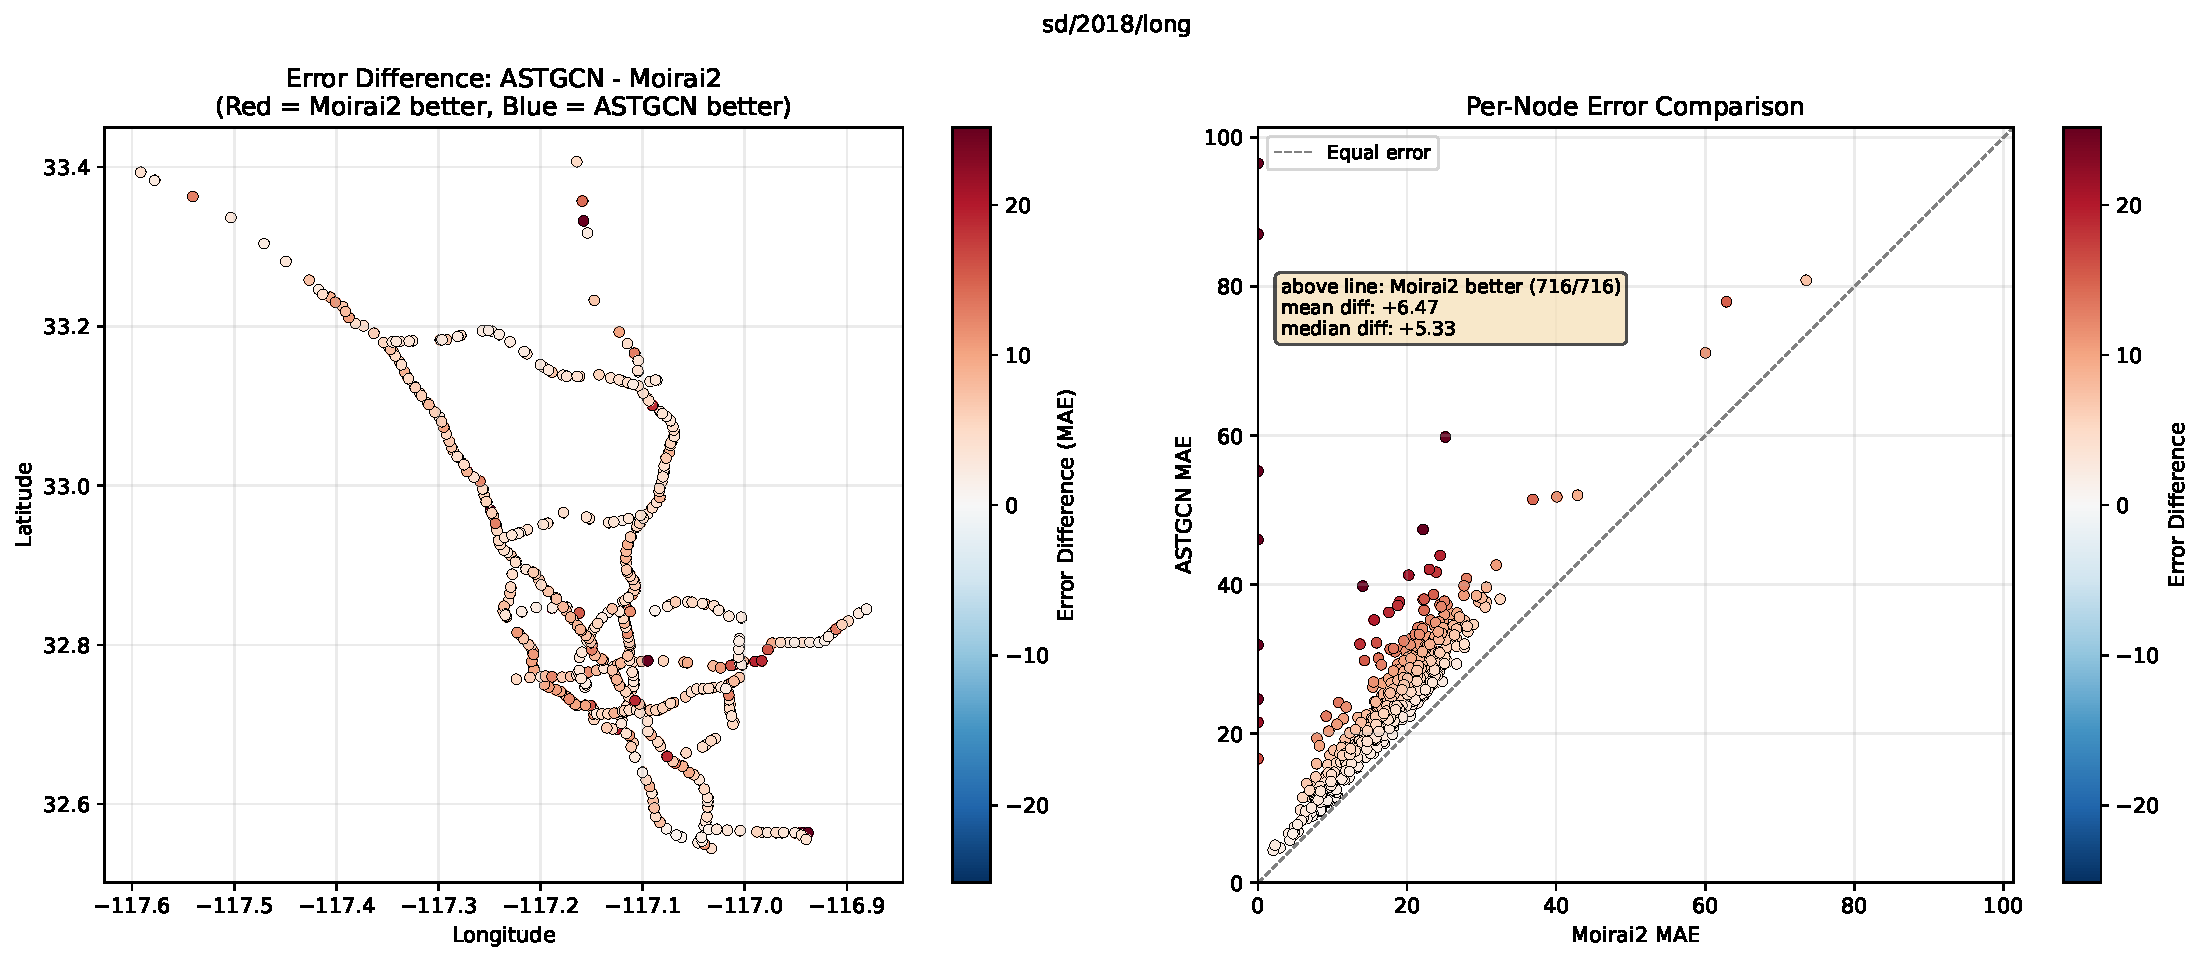
\includegraphics[width=\linewidth]{figs/node_error_astgcn_moirai2.pdf}
  \caption{\texttt{ASTGCN} against \texttt{Moirai-2}: the pretrained model wins
  on 716 of 716 sensors.}
\end{subfigure}
\\[6pt]
\begin{subfigure}[t]{\linewidth}
  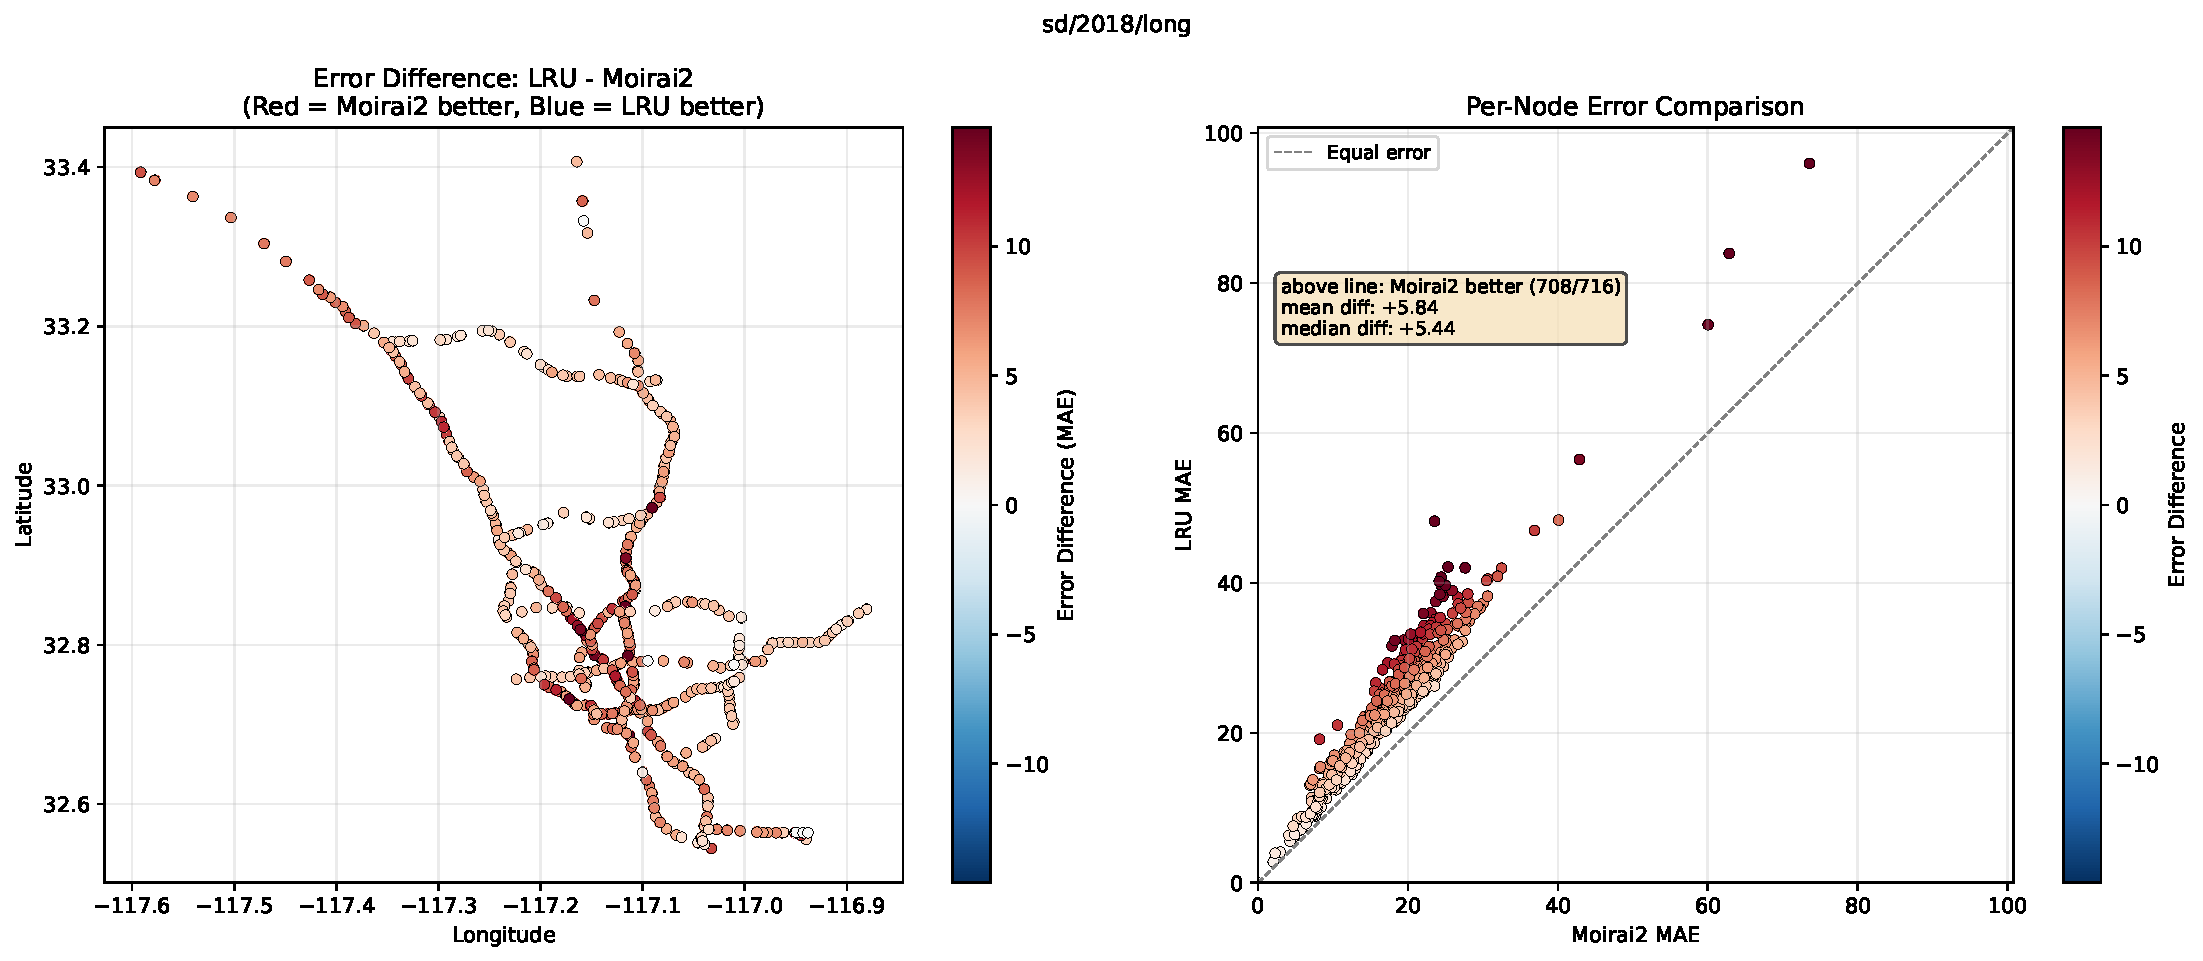
\includegraphics[width=\linewidth]{figs/node_error_lru_moirai2.pdf}
  \caption{\texttt{LRU} against \texttt{Moirai-2}: 708 of 716.}
\end{subfigure}
\caption{Per-sensor MAE on SD~2018 over all 716 sensors, same windows as
Figure~\ref{fig:app_hourly}. In each row, left is the spatial distribution of
the difference and right the per-sensor scatter against the $y=x$ line.
\emph{The pretrained model's advantage is uniform, not carried by outliers.}
\texttt{Moirai-2} (mean MAE $17.07$) is better than \texttt{ASTGCN} ($23.53$) on
\emph{every} sensor---a matched-pairs rank-biserial correlation of exactly
$+1.00$---and better than \texttt{LRU} ($22.90$) on $708$ of $716$ ($98.9\%$,
$r = +0.98$); both Wilcoxon signed-rank tests reject equality at
$p < 10^{-100}$. That this is a real property of the comparison and not of the
metric is clear from the same test applied to the two task-trained models:
\texttt{LRU} has a lower mean MAE than \texttt{ASTGCN} by $0.63$, but it wins
on only $330$ of $716$ sensors ($46.1\%$), the median difference runs the other
way, and Wilcoxon does not reject equality ($p = 0.092$). A mean gap can
therefore be uniform or an artifact of a few sensors, and on SD only the
pretrained model's is the former---consistent with
Section~\ref{app:extended:tables}, where SD is the one subset on which the
task-trained families do not separate.}
\label{fig:app_node}
\end{figure*}

\subsection{Information conditioning and the cost of full-graph inference}
\label{app:extended:asymmetry}

The two families are not conditioned on the same information. A spatiotemporal
GNN observes every sensor in the network simultaneously in a single forward
pass; the SSMs, linear forecasters and foundation models observe the history of
one sensor at a time and nothing else. Under identical data, splits, context
lengths and evaluation protocol, the graph models are strictly better informed
at prediction time.

That advantage does not appear in the results. On GBA and GLA, in both years,
the best graph-free model attains a lower MAE than \emph{every} executable graph
model at \emph{every} horizon---twelve comparisons out of twelve, with margins
that widen as the horizon grows (at $H{=}12$ on GLA~2019, 18.17 against 28.93).
This is not an artifact of pretraining scale: restricting the comparison to the
task-trained SSMs, which see the same training data under the same budget and
simply have no access to the adjacency, the same ordering holds at every horizon
on GLA and CA and at all but one on GBA. Whatever the graph contributes on these
networks, it is not being converted into accuracy.

The constraint is also unevenly distributed inside the family. The most accurate
graph model on SD, \texttt{DGCRN}, cannot be run on GLA or CA at all, and
\texttt{D2STGNN} cannot be run beyond SD---though the exclusion is not total,
since \texttt{AGCRN} places second on SD and executes everywhere. The cost of
full-graph inference is therefore not only that a forward pass is expensive and
needs a synchronized network-wide snapshot: the memory footprint removes some of
the family's most competitive members from consideration before accuracy is
measured, while per-series models remain available at every scale.

\subsection{Year-over-year stability}
\label{app:extended:years}

Ranking the shared methods by Avg MAE within each region and comparing 2018 to
2019 gives Spearman $\rho = 0.98$ on SD, $0.97$ on GBA, $0.95$ on GLA and
$0.87$ on CA. The family-level conclusions above are therefore not an artifact
of the year, which is the check the main text's single-year tables cannot
perform. Individual methods are much less stable than families---\texttt{STTN}
moves up four to eleven places depending on the subset, \texttt{AGCRN} up
eight on CA and \texttt{DSTAGNN} down six on GBA---but no such movement
changes which family leads. CA is the least stable subset
($\rho = 0.87$ against $0.95$--$0.98$ elsewhere), and
Section~\ref{app:extended:ca} locates the reason: the lag-feature regressors
and the ensembles built on them degrade far more between the two years than any
other family does. A single-year, single-region table is thus
adequate for choosing a \emph{family} and unreliable for ranking neighbours
within one, which is the paper's own thesis about fragmented protocols applied
to itself.

\begin{insightbox}
\textit{Takeaway:} Across four subsets and two years, pretrained foundation
models lead at every horizon rather than only at long ones---\texttt{Sundial} is
first in all eight cells (Wilcoxon $p = 0.0078$ against the best graph model in
each)---but the family is not uniform, and \texttt{TimesFM}, the largest model
evaluated, loses to the best state-space model everywhere. The graph models are
the only family conditioned on the whole network at inference time, yet on GBA
and GLA every executable one is beaten at every horizon by models that see a
single sensor, including task-trained SSMs that differ from them chiefly in
having no adjacency; on CA they trail the state-space models by $19$--$29\%$,
and their most accurate member cannot be run there at all. Spatial message passing is thus both
unrewarded at scale here and, for its strongest variants, unavailable---though
even with eight region-years the omnibus post-hoc test still cannot separate the
graph and pretrained families at $\alpha = 0.05$ (rank gap $2.75$ against a
critical difference of $2.85$), so the ordering is consistent rather than
individually certified.
\end{insightbox}

\begin{table*}[t]
\centering
\caption{Run coverage. \ding{51}~= evaluated; \ding{55}~= no usable result for that subset, shown as ``-'' in the tables that follow.}
\label{tab:app_coverage}
\resizebox{\textwidth}{!}{
\begin{tabular}{c|c|c|c|c|c|c|c|c|c}
\toprule
Category & Method & SD 2019 & SD 2018 & GBA 2019 & GBA 2018 & GLA 2019 & GLA 2018 & CA 2019 & CA 2018 \\
\midrule
\multirow{3}{*}{Simple Baselines} & HL & \ding{51} & \ding{51} & \ding{51} & \ding{51} & \ding{51} & \ding{51} & \ding{51} & \ding{51} \\
 & Naive & \ding{51} & \ding{51} & \ding{51} & \ding{51} & \ding{51} & \ding{51} & \ding{51} & \ding{51} \\
 & Seasonal Naive & \ding{51} & \ding{51} & \ding{51} & \ding{51} & \ding{51} & \ding{51} & \ding{51} & \ding{51} \\
\midrule
\multirow{4}{*}{ML Baselines} & Ridge & \ding{51} & \ding{51} & \ding{51} & \ding{51} & \ding{51} & \ding{51} & \ding{51} & \ding{51} \\
 & Random Forest & \ding{51} & \ding{51} & \ding{51} & \ding{51} & \ding{51} & \ding{51} & \ding{51} & \ding{51} \\
 & Linear Regression & \ding{51} & \ding{51} & \ding{51} & \ding{51} & \ding{51} & \ding{51} & \ding{51} & \ding{51} \\
 & LightGBM & \ding{51} & \ding{51} & \ding{51} & \ding{51} & \ding{51} & \ding{51} & \ding{51} & \ding{51} \\
\midrule
\multirow{3}{*}{Ensembles} & Median & \ding{51} & \ding{51} & \ding{51} & \ding{51} & \ding{51} & \ding{51} & \ding{51} & \ding{51} \\
 & Mean & \ding{51} & \ding{51} & \ding{51} & \ding{51} & \ding{51} & \ding{51} & \ding{51} & \ding{51} \\
 & Weighted & \ding{51} & \ding{51} & \ding{51} & \ding{51} & \ding{51} & \ding{51} & \ding{51} & \ding{51} \\
\midrule
\multirow{4}{*}{SSM} & Linear SSM & \ding{51} & \ding{51} & \ding{51} & \ding{51} & \ding{51} & \ding{51} & \ding{51} & \ding{51} \\
 & LRU & \ding{51} & \ding{51} & \ding{51} & \ding{51} & \ding{51} & \ding{51} & \ding{51} & \ding{51} \\
 & S4 & \ding{51} & \ding{51} & \ding{51} & \ding{51} & \ding{51} & \ding{51} & \ding{51} & \ding{51} \\
 & Mamba-v2 & \ding{51} & \ding{51} & \ding{51} & \ding{51} & \ding{51} & \ding{51} & \ding{51} & \ding{51} \\
\midrule
\multirow{2}{*}{Linear} & DLinear & \ding{51} & \ding{51} & \ding{51} & \ding{51} & \ding{51} & \ding{51} & \ding{51} & \ding{51} \\
 & NLinear & \ding{51} & \ding{51} & \ding{51} & \ding{51} & \ding{51} & \ding{51} & \ding{51} & \ding{51} \\
\midrule
\multirow{7}{*}{Foundation Models} & FlowState & \ding{55} & \ding{55} & \ding{55} & \ding{55} & \ding{55} & \ding{55} & \ding{55} & \ding{55} \\
 & Chronos-Bolt & \ding{51} & \ding{51} & \ding{51} & \ding{51} & \ding{51} & \ding{51} & \ding{51} & \ding{51} \\
 & Kairos & \ding{51} & \ding{51} & \ding{51} & \ding{51} & \ding{51} & \ding{51} & \ding{51} & \ding{51} \\
 & Moirai-2 & \ding{51} & \ding{51} & \ding{51} & \ding{51} & \ding{51} & \ding{51} & \ding{51} & \ding{51} \\
 & Moirai-Small & \ding{51} & \ding{51} & \ding{51} & \ding{51} & \ding{51} & \ding{51} & \ding{51} & \ding{51} \\
 & TimesFM & \ding{51} & \ding{51} & \ding{51} & \ding{51} & \ding{51} & \ding{51} & \ding{51} & \ding{51} \\
 & Sundial & \ding{51} & \ding{51} & \ding{51} & \ding{51} & \ding{51} & \ding{51} & \ding{51} & \ding{51} \\
\midrule
\multirow{10}{*}{GNN-based} & AGCRN & \ding{51} & \ding{51} & \ding{51} & \ding{51} & \ding{51} & \ding{51} & \ding{51} & \ding{51} \\
 & ASTGCN & \ding{51} & \ding{51} & \ding{51} & \ding{51} & \ding{51} & \ding{51} & \ding{51} & \ding{51} \\
 & D2STGNN & \ding{51} & \ding{51} & \ding{55} & \ding{55} & \ding{55} & \ding{55} & \ding{55} & \ding{55} \\
 & DCRNN & \ding{51} & \ding{51} & \ding{51} & \ding{51} & \ding{51} & \ding{51} & \ding{51} & \ding{51} \\
 & DGCRN & \ding{51} & \ding{51} & \ding{55} & \ding{51} & \ding{55} & \ding{55} & \ding{55} & \ding{55} \\
 & DSTAGNN & \ding{51} & \ding{51} & \ding{51} & \ding{51} & \ding{51} & \ding{51} & \ding{51} & \ding{51} \\
 & GWNET & \ding{51} & \ding{51} & \ding{51} & \ding{51} & \ding{51} & \ding{51} & \ding{51} & \ding{51} \\
 & STGCN & \ding{51} & \ding{51} & \ding{51} & \ding{51} & \ding{51} & \ding{51} & \ding{51} & \ding{51} \\
 & STGODE & \ding{55} & \ding{55} & \ding{55} & \ding{55} & \ding{55} & \ding{55} & \ding{55} & \ding{55} \\
 & STTN & \ding{51} & \ding{51} & \ding{51} & \ding{51} & \ding{51} & \ding{51} & \ding{51} & \ding{51} \\
\bottomrule
\end{tabular}
}
\end{table*}

\begin{table*}[t]
\centering
\caption{Performance Comparison of Forecasting Methods (San Diego Data, 2019)}
\label{tab:app_sd_2019}
\resizebox{\textwidth}{!}{
\begin{tabular}{c|c|c|c|c|c|c|c|c|c|c|c|c|c}
\toprule
Category & Method & H3 MAE & H3 RMSE & H3 MAPE & H6 MAE & H6 RMSE & H6 MAPE & H12 MAE & H12 RMSE & H12 MAPE & Avg MAE & Avg RMSE & Avg MAPE \\
\midrule
\multirow{3}{*}{Simple Baselines} & HL & 33.61 & 50.96 & 20.74\% & 57.79 & 84.88 & 37.69\% & 101.78 & 140.10 & 76.82\% & 60.80 & 87.36 & 41.84\% \\
 & Naive & 22.48 & 33.04 & 10.83\% & 34.41 & 52.49 & 24.01\% & 50.48 & 76.01 & 38.27\% & 35.79 & 53.85 & 24.37\% \\
 & Seasonal Naive & 38.91 & 67.13 & 27.69\% & 31.14 & 56.11 & 23.33\% & 45.13 & 76.60 & 26.21\% & 38.39 & 66.61 & 25.74\% \\
\midrule
\multirow{4}{*}{ML Baselines} & Ridge & 19.76 & 30.01 & 9.63\% & 26.84 & 41.61 & 23.38\% & 37.11 & 57.54 & 37.29\% & 27.90 & 43.05 & 23.43\% \\
 & Random Forest & 21.45 & 32.29 & 9.55\% & 27.29 & 43.95 & 17.45\% & 34.63 & 56.59 & 20.69\% & 27.79 & 44.28 & 15.90\% \\
 & Linear Regression & 19.76 & 30.01 & 9.63\% & 26.84 & 41.61 & 23.38\% & 37.10 & 57.54 & 37.29\% & 27.90 & 43.05 & 23.43\% \\
 & LightGBM & 22.85 & 33.65 & 10.65\% & 29.53 & 44.74 & 23.11\% & 37.96 & 57.59 & 30.60\% & 30.11 & 45.33 & 21.45\% \\
\midrule
\multirow{3}{*}{Ensembles} & Median & 18.49 & 28.19 & 8.75\% & 23.55 & 37.02 & 18.56\% & 31.71 & 48.59 & 27.21\% & 24.58 & 37.93 & 18.17\% \\
 & Mean & 19.99 & 30.59 & 11.89\% & 22.49 & 34.89 & 18.50\% & 30.79 & 46.49 & 26.33\% & 24.42 & 37.32 & 18.91\% \\
 & Weighted & 19.17 & 28.87 & 10.46\% & 23.23 & 35.95 & 18.60\% & 30.89 & 46.97 & 26.33\% & 24.43 & 37.26 & 18.46\% \\
\midrule
\multirow{4}{*}{SSM} & Linear SSM & 16.65 & 26.20 & 7.90\% & 18.39 & 31.80 & 12.88\% & 24.32 & 42.91 & 15.12\% & 19.79 & 33.64 & 11.97\% \\
 & LRU & 16.61 & 26.33 & 7.59\% & 17.12 & 29.14 & 11.45\% & 21.49 & 36.95 & 13.38\% & 18.41 & 30.81 & 10.81\% \\
 & S4 & 17.29 & 26.65 & 7.59\% & 17.44 & 29.28 & 11.02\% & 21.77 & 36.45 & 12.67\% & 18.83 & 30.79 & 10.43\% \\
 & Mamba-v2 & 16.62 & 26.28 & 7.91\% & 17.58 & 30.72 & 11.49\% & 21.57 & 35.29 & 13.51\% & 18.59 & 30.76 & 10.97\% \\
\midrule
\multirow{2}{*}{Linear} & DLinear & 17.39 & 27.87 & 8.61\% & 17.84 & 30.58 & 12.43\% & 26.32 & 46.34 & 15.95\% & 20.52 & 34.93 & 12.33\% \\
 & NLinear & 17.34 & 27.81 & 8.63\% & 17.84 & 30.69 & 12.41\% & 26.41 & 46.59 & 16.00\% & 20.53 & 35.03 & 12.35\% \\
\midrule
\multirow{7}{*}{Foundation Models} & FlowState & - & - & - & - & - & - & - & - & - & - & - & - \\
 & Chronos-Bolt & 16.46 & 26.07 & 7.12\% & 15.94 & \underline{27.40} & \underline{9.64\%} & \underline{17.06} & \underline{29.19} & \underline{10.00\%} & 16.49 & \underline{27.55} & 8.92\% \\
 & Kairos & 16.86 & 26.12 & 7.48\% & 17.25 & 28.79 & 10.95\% & 18.80 & 31.10 & 11.63\% & 17.64 & 28.67 & 10.02\% \\
 & Moirai-2 & 15.83 & \underline{25.08} & \underline{6.94\%} & \underline{15.87} & 27.84 & 9.65\% & 17.14 & 30.09 & 10.03\% & \underline{16.28} & 27.67 & \underline{8.87\%} \\
 & Moirai-Small & 26.23 & 41.09 & 16.65\% & 35.27 & 51.24 & 25.17\% & 59.90 & 90.04 & 38.81\% & 40.47 & 60.79 & 26.88\% \\
 & TimesFM & 16.55 & 28.36 & 9.55\% & 19.29 & 30.85 & 11.52\% & 25.37 & 41.99 & 14.67\% & 19.75 & 33.31 & 11.69\% \\
 & Sundial & \textbf{15.12} & \textbf{24.63} & \textbf{6.63\%} & \textbf{14.74} & \textbf{25.91} & \textbf{9.06\%} & \textbf{16.48} & \textbf{28.67} & \textbf{9.66\%} & \textbf{15.45} & \textbf{26.40} & \textbf{8.45\%} \\
\midrule
\multirow{10}{*}{GNN-based} & AGCRN & 15.84 & 27.47 & 11.68\% & 18.02 & 31.09 & 12.57\% & 21.47 & 38.79 & 15.71\% & 18.12 & 31.83 & 13.12\% \\
 & ASTGCN & 20.88 & 32.30 & 14.23\% & 28.42 & 42.43 & 19.52\% & 37.16 & 55.44 & 29.42\% & 27.83 & 42.00 & 20.20\% \\
 & D2STGNN & 15.78 & 25.83 & 10.81\% & 18.31 & 30.20 & 13.00\% & 22.36 & 37.68 & 16.61\% & 18.44 & 30.56 & 13.14\% \\
 & DCRNN & 17.14 & 27.46 & 11.07\% & 20.92 & 33.28 & 13.87\% & 26.67 & 42.34 & 18.66\% & 21.02 & 33.50 & 14.10\% \\
 & DGCRN & \underline{15.18} & 25.21 & 10.08\% & 17.54 & 29.33 & 11.78\% & 21.28 & 35.92 & 14.86\% & 17.65 & 29.54 & 11.97\% \\
 & DSTAGNN & 17.64 & 28.43 & 11.60\% & 21.32 & 34.66 & 13.96\% & 26.48 & 42.97 & 18.38\% & 21.29 & 34.49 & 14.27\% \\
 & GWNET & 15.57 & 25.44 & 10.32\% & 18.26 & 30.03 & 11.97\% & 21.90 & 36.28 & 15.33\% & 18.20 & 29.94 & 12.26\% \\
 & STGCN & 17.55 & 30.16 & 12.32\% & 19.48 & 33.52 & 13.46\% & 23.05 & 40.35 & 16.22\% & 19.72 & 34.11 & 13.79\% \\
 & STGODE & - & - & - & - & - & - & - & - & - & - & - & - \\
 & STTN & 16.38 & 26.26 & 11.09\% & 18.74 & 30.67 & 12.56\% & 22.93 & 39.33 & 16.30\% & 18.89 & 31.26 & 13.04\% \\
\bottomrule
\end{tabular}
}
\end{table*}

\begin{table*}[t]
\centering
\caption{Performance Comparison of Forecasting Methods (San Diego Data, 2018)}
\label{tab:app_sd_2018}
\resizebox{\textwidth}{!}{
\begin{tabular}{c|c|c|c|c|c|c|c|c|c|c|c|c|c}
\toprule
Category & Method & H3 MAE & H3 RMSE & H3 MAPE & H6 MAE & H6 RMSE & H6 MAPE & H12 MAE & H12 RMSE & H12 MAPE & Avg MAE & Avg RMSE & Avg MAPE \\
\midrule
\multirow{3}{*}{Simple Baselines} & HL & 33.68 & 50.98 & 20.36\% & 58.26 & 85.63 & 37.20\% & 103.17 & 141.99 & 75.92\% & 61.37 & 88.15 & 41.27\% \\
 & Naive & 21.11 & 31.17 & 10.44\% & 30.61 & 44.56 & 22.61\% & 45.34 & 64.60 & 35.35\% & 32.35 & 46.78 & 22.80\% \\
 & Seasonal Naive & 35.98 & 52.31 & 16.27\% & 37.46 & 57.49 & 24.53\% & 36.03 & 54.09 & 22.09\% & 36.49 & 54.63 & 20.96\% \\
\midrule
\multirow{4}{*}{ML Baselines} & Ridge & 18.48 & 28.69 & 9.45\% & 23.65 & 35.91 & 23.36\% & 31.78 & 45.67 & 37.63\% & 24.64 & 36.76 & 23.48\% \\
 & Random Forest & 20.17 & 30.23 & 9.33\% & 25.28 & 40.13 & 17.75\% & 35.31 & 56.99 & 23.33\% & 26.92 & 42.45 & 16.80\% \\
 & Linear Regression & 18.48 & 28.69 & 9.45\% & 23.65 & 35.91 & 23.36\% & 31.78 & 45.67 & 37.63\% & 24.64 & 36.76 & 23.48\% \\
 & LightGBM & 20.97 & 30.96 & 10.17\% & 27.65 & 40.99 & 24.07\% & 38.62 & 57.29 & 33.06\% & 29.08 & 43.08 & 22.43\% \\
\midrule
\multirow{3}{*}{Ensembles} & Median & 17.52 & 27.12 & 8.65\% & 21.65 & 32.69 & 19.64\% & 26.82 & 37.87 & 27.30\% & 22.00 & 32.56 & 18.53\% \\
 & Mean & 18.16 & 27.56 & 8.85\% & 21.44 & 32.06 & 18.85\% & 26.54 & 37.26 & 26.16\% & 22.05 & 32.29 & 17.95\% \\
 & Weighted & 17.46 & 26.82 & 8.49\% & 21.15 & 31.92 & 18.65\% & 27.43 & 39.23 & 26.68\% & 22.01 & 32.66 & 17.94\% \\
\midrule
\multirow{4}{*}{SSM} & Linear SSM & 16.14 & 26.22 & 7.18\% & 16.83 & 28.43 & 11.16\% & 21.16 & 33.95 & 14.16\% & 18.04 & 29.53 & 10.83\% \\
 & LRU & 15.64 & 25.52 & 7.12\% & 16.24 & 27.62 & 11.05\% & 19.03 & 30.38 & 13.22\% & 16.97 & 27.84 & 10.46\% \\
 & S4 & 16.65 & 26.50 & 7.48\% & 18.25 & 32.39 & 11.76\% & 18.43 & 30.65 & 12.00\% & 17.78 & 29.85 & 10.41\% \\
 & Mamba-v2 & 16.09 & 25.83 & 7.28\% & 17.35 & 30.42 & 11.25\% & 18.66 & 31.77 & 12.45\% & 17.37 & 29.34 & 10.33\% \\
\midrule
\multirow{2}{*}{Linear} & DLinear & 15.84 & 26.20 & 7.27\% & 18.27 & 30.99 & 12.46\% & 21.90 & 34.64 & 14.36\% & 18.67 & 30.61 & 11.36\% \\
 & NLinear & 15.81 & 26.19 & 7.23\% & 17.94 & 30.70 & 12.25\% & 21.60 & 34.35 & 14.19\% & 18.45 & 30.41 & 11.22\% \\
\midrule
\multirow{7}{*}{Foundation Models} & FlowState & - & - & - & - & - & - & - & - & - & - & - & - \\
 & Chronos-Bolt & 15.63 & 25.68 & 7.07\% & \underline{14.50} & 25.16 & \underline{9.31\%} & 14.61 & 24.05 & 9.45\% & 14.91 & 24.96 & \underline{8.61\%} \\
 & Kairos & 15.23 & 24.36 & 7.08\% & 14.90 & \underline{24.49} & 10.78\% & 15.26 & 24.12 & 10.73\% & 15.13 & \underline{24.32} & 9.53\% \\
 & Moirai-2 & 15.25 & 25.11 & \underline{6.96\%} & 14.53 & 24.58 & 10.07\% & \underline{14.50} & \underline{23.56} & \underline{9.44\%} & \underline{14.76} & 24.42 & 8.82\% \\
 & Moirai-Small & 21.70 & 32.89 & 14.88\% & 30.00 & 43.12 & 23.08\% & 42.91 & 59.49 & 35.91\% & 31.54 & 45.17 & 24.62\% \\
 & TimesFM & \underline{14.52} & \textbf{22.62} & 9.15\% & 17.51 & 27.09 & 11.70\% & 23.47 & 37.97 & 15.21\% & 17.75 & 28.89 & 11.60\% \\
 & Sundial & \textbf{14.24} & 23.62 & \textbf{6.54\%} & \textbf{13.45} & \textbf{23.40} & \textbf{8.91\%} & \textbf{13.79} & \textbf{22.78} & \textbf{8.98\%} & \textbf{13.83} & \textbf{23.27} & \textbf{8.14\%} \\
\midrule
\multirow{10}{*}{GNN-based} & AGCRN & 14.80 & 23.82 & 9.11\% & 17.21 & 27.84 & 10.64\% & 20.79 & 35.18 & 10.81\% & 17.25 & 28.31 & 10.05\% \\
 & ASTGCN & 18.75 & 29.82 & 11.31\% & 22.29 & 34.90 & 13.69\% & 28.25 & 45.51 & 18.13\% & 22.55 & 35.88 & 13.99\% \\
 & D2STGNN & 14.91 & 23.92 & 9.14\% & 17.27 & 27.70 & 10.65\% & 21.01 & 34.22 & 13.25\% & 17.38 & 28.03 & 10.78\% \\
 & DCRNN & 15.75 & 24.96 & 9.80\% & 18.70 & 29.45 & 11.92\% & 23.53 & 37.53 & 15.55\% & 18.88 & 29.94 & 12.10\% \\
 & DGCRN & 14.58 & \underline{23.36} & 8.91\% & 17.03 & 27.46 & 10.50\% & 20.88 & 35.29 & 13.28\% & 17.13 & 28.04 & 10.65\% \\
 & DSTAGNN & 16.92 & 26.60 & 10.51\% & 20.20 & 31.57 & 13.27\% & 24.58 & 38.95 & 16.47\% & 20.11 & 31.65 & 13.05\% \\
 & GWNET & 14.76 & 23.64 & 9.67\% & 17.37 & 28.03 & 11.30\% & 21.23 & 36.52 & 14.25\% & 17.41 & 28.68 & 11.48\% \\
 & STGCN & 16.23 & 25.83 & 10.08\% & 18.55 & 29.78 & 11.36\% & 21.51 & 35.81 & 13.50\% & 18.45 & 29.89 & 11.45\% \\
 & STGODE & - & - & - & - & - & - & - & - & - & - & - & - \\
 & STTN & 16.05 & 25.22 & 10.03\% & 19.28 & 30.81 & 12.04\% & 23.25 & 39.82 & 14.87\% & 19.09 & 31.11 & 12.03\% \\
\bottomrule
\end{tabular}
}
\end{table*}

\begin{table*}[t]
\centering
\caption{Performance Comparison of Forecasting Methods (Bay Area Data, 2019)}
\label{tab:app_gba_2019}
\resizebox{\textwidth}{!}{
\begin{tabular}{c|c|c|c|c|c|c|c|c|c|c|c|c|c}
\toprule
Category & Method & H3 MAE & H3 RMSE & H3 MAPE & H6 MAE & H6 RMSE & H6 MAPE & H12 MAE & H12 RMSE & H12 MAPE & Avg MAE & Avg RMSE & Avg MAPE \\
\midrule
\multirow{3}{*}{Simple Baselines} & HL & 32.55 & 48.38 & 22.73\% & 53.78 & 77.03 & 42.93\% & 92.67 & 126.19 & 92.79\% & 56.43 & 79.78 & 48.80\% \\
 & Naive & 22.22 & 33.33 & 10.99\% & 33.51 & 48.67 & 26.48\% & 50.89 & 75.02 & 45.46\% & 35.54 & 52.34 & 27.64\% \\
 & Seasonal Naive & 40.72 & 67.18 & 16.15\% & 35.88 & 60.18 & 18.64\% & 49.81 & 77.84 & 28.16\% & 42.14 & 68.40 & 20.98\% \\
\midrule
\multirow{4}{*}{ML Baselines} & Ridge & 19.25 & 30.13 & 9.37\% & 26.29 & 38.65 & 26.92\% & 38.80 & 56.42 & 45.59\% & 28.11 & 41.73 & 27.29\% \\
 & Random Forest & 22.04 & 33.58 & 9.39\% & 27.51 & 42.43 & 19.18\% & 35.11 & 54.36 & 23.73\% & 28.22 & 43.46 & 17.43\% \\
 & Linear Regression & 19.25 & 30.14 & 9.37\% & 26.29 & 38.65 & 26.92\% & 38.80 & 56.42 & 45.59\% & 28.11 & 41.74 & 27.29\% \\
 & LightGBM & 23.18 & 34.37 & 10.56\% & 29.14 & 42.24 & 27.69\% & 38.04 & 55.90 & 36.41\% & 30.12 & 44.17 & 24.89\% \\
\midrule
\multirow{3}{*}{Ensembles} & Median & 18.52 & 29.26 & 8.59\% & 23.28 & 34.96 & 20.94\% & 33.76 & 49.46 & 33.78\% & 25.19 & 37.89 & 21.10\% \\
 & Mean & 19.89 & 31.14 & 8.81\% & 22.17 & 33.49 & 19.07\% & 32.59 & 47.53 & 31.57\% & 24.88 & 37.39 & 19.82\% \\
 & Weighted & 19.04 & 29.67 & 8.56\% & 22.79 & 34.13 & 19.95\% & 32.35 & 47.28 & 31.71\% & 24.73 & 37.03 & 20.07\% \\
\midrule
\multirow{4}{*}{SSM} & Linear SSM & 16.26 & 26.96 & 7.21\% & 18.69 & 29.99 & 13.83\% & 27.22 & 44.20 & 18.70\% & 20.72 & 33.72 & 13.25\% \\
 & LRU & 15.88 & 26.83 & 7.02\% & 17.71 & 28.71 & 13.18\% & 25.36 & 40.81 & 17.96\% & 19.65 & 32.12 & 12.72\% \\
 & S4 & 16.51 & 28.01 & 7.11\% & 18.15 & 29.98 & 12.04\% & 24.52 & 39.49 & 15.86\% & 19.73 & 32.49 & 11.67\% \\
 & Mamba-v2 & 15.91 & 27.31 & 6.92\% & 17.88 & 29.87 & 11.36\% & 24.11 & 38.90 & 15.93\% & 19.30 & 32.03 & 11.40\% \\
\midrule
\multirow{2}{*}{Linear} & DLinear & 18.23 & 29.38 & 8.23\% & 18.46 & 30.54 & 13.18\% & 23.02 & 37.04 & 17.30\% & 19.90 & 32.32 & 12.90\% \\
 & NLinear & 17.73 & 28.77 & 8.03\% & 19.31 & 31.45 & 13.66\% & 23.10 & 37.33 & 17.30\% & 20.05 & 32.52 & 13.00\% \\
\midrule
\multirow{7}{*}{Foundation Models} & FlowState & - & - & - & - & - & - & - & - & - & - & - & - \\
 & Chronos-Bolt & 15.01 & 25.85 & 6.33\% & \underline{15.75} & 26.21 & 10.69\% & 19.45 & 31.75 & \underline{12.99\%} & 16.74 & 27.94 & \underline{10.00\%} \\
 & Kairos & 14.85 & \textbf{25.44} & 6.27\% & 15.78 & \underline{26.15} & 10.65\% & 19.90 & 31.65 & 13.60\% & 16.84 & \underline{27.75} & 10.17\% \\
 & Moirai-2 & \underline{14.84} & 25.78 & \underline{6.26\%} & 15.76 & 26.62 & \underline{10.64\%} & \underline{19.28} & \underline{31.60} & 13.17\% & \underline{16.63} & 28.00 & 10.02\% \\
 & Moirai-Small & 25.74 & 37.07 & 20.10\% & 37.84 & 53.26 & 31.56\% & 56.92 & 79.51 & 49.82\% & 40.17 & 56.61 & 33.83\% \\
 & TimesFM & 17.83 & 28.25 & 11.91\% & 22.46 & 35.62 & 15.43\% & 27.69 & 44.09 & 17.93\% & 22.46 & 36.29 & 15.13\% \\
 & Sundial & \textbf{14.32} & \underline{25.55} & \textbf{5.94\%} & \textbf{15.11} & \textbf{25.98} & \textbf{10.29\%} & \textbf{19.02} & \textbf{31.43} & \textbf{12.88\%} & \textbf{16.15} & \textbf{27.65} & \textbf{9.70\%} \\
\midrule
\multirow{10}{*}{GNN-based} & AGCRN & 18.43 & 30.46 & 14.04\% & 21.40 & 34.99 & 16.81\% & 24.99 & 40.60 & 21.03\% & 21.21 & 34.74 & 16.89\% \\
 & ASTGCN & 20.77 & 30.86 & 18.14\% & 29.16 & 42.73 & 25.34\% & 37.29 & 56.13 & 31.25\% & 28.33 & 42.12 & 24.65\% \\
 & D2STGNN & - & - & - & - & - & - & - & - & - & - & - & - \\
 & DCRNN & 24.41 & 37.05 & 25.08\% & 30.32 & 45.59 & 33.23\% & 44.03 & 68.30 & 39.68\% & 31.86 & 48.66 & 31.72\% \\
 & DGCRN & - & - & - & - & - & - & - & - & - & - & - & - \\
 & DSTAGNN & 19.81 & 31.38 & 15.85\% & 24.55 & 38.26 & 22.28\% & 28.25 & 44.31 & 24.30\% & 23.65 & 37.16 & 20.19\% \\
 & GWNET & 18.45 & 29.86 & 14.58\% & 22.57 & 35.40 & 19.76\% & 28.20 & 43.40 & 27.94\% & 22.50 & 35.43 & 19.99\% \\
 & STGCN & 20.83 & 34.08 & 16.34\% & 23.27 & 38.09 & 18.32\% & 26.51 & 43.71 & 21.82\% & 23.20 & 38.06 & 18.52\% \\
 & STGODE & - & - & - & - & - & - & - & - & - & - & - & - \\
 & STTN & 17.74 & 27.93 & 12.17\% & 23.74 & 37.51 & 16.48\% & 28.97 & 45.29 & 19.42\% & 23.41 & 36.73 & 16.43\% \\
\bottomrule
\end{tabular}
}
\end{table*}

\begin{table*}[t]
\centering
\caption{Performance Comparison of Forecasting Methods (Bay Area Data, 2018)}
\label{tab:app_gba_2018}
\resizebox{\textwidth}{!}{
\begin{tabular}{c|c|c|c|c|c|c|c|c|c|c|c|c|c}
\toprule
Category & Method & H3 MAE & H3 RMSE & H3 MAPE & H6 MAE & H6 RMSE & H6 MAPE & H12 MAE & H12 RMSE & H12 MAPE & Avg MAE & Avg RMSE & Avg MAPE \\
\midrule
\multirow{3}{*}{Simple Baselines} & HL & 33.45 & 50.54 & 23.96\% & 54.59 & 78.72 & 45.01\% & 92.79 & 126.78 & 96.88\% & 57.11 & 81.36 & 51.09\% \\
 & Naive & 22.67 & 34.31 & 12.54\% & 29.75 & 43.22 & 27.19\% & 45.92 & 65.74 & 47.03\% & 32.78 & 47.76 & 28.92\% \\
 & Seasonal Naive & 38.11 & 59.29 & 19.11\% & 37.92 & 59.31 & 28.61\% & 37.73 & 59.11 & 28.39\% & 37.92 & 59.24 & 25.37\% \\
\midrule
\multirow{4}{*}{ML Baselines} & Ridge & 20.29 & 32.08 & 11.58\% & 23.89 & 35.91 & 31.66\% & 33.79 & 49.01 & 52.99\% & 25.99 & 39.00 & 32.08\% \\
 & Random Forest & 21.86 & 33.13 & 11.43\% & 26.09 & 39.56 & 25.57\% & 35.88 & 55.22 & 33.73\% & 27.94 & 42.64 & 23.58\% \\
 & Linear Regression & 20.19 & 32.08 & 11.58\% & 23.89 & 35.91 & 31.66\% & 33.79 & 49.01 & 52.99\% & 25.96 & 39.00 & 32.08\% \\
 & LightGBM & 22.54 & 33.59 & 12.38\% & 27.31 & 39.89 & 35.87\% & 38.99 & 56.59 & 49.66\% & 29.61 & 43.36 & 32.64\% \\
\midrule
\multirow{3}{*}{Ensembles} & Median & 19.37 & 30.51 & 10.78\% & 22.24 & 33.23 & 27.08\% & 29.47 & 43.11 & 40.53\% & 23.69 & 35.62 & 26.13\% \\
 & Mean & 19.92 & 30.89 & 11.05\% & 22.54 & 33.31 & 25.95\% & 28.94 & 42.07 & 38.37\% & 23.80 & 35.42 & 25.12\% \\
 & Weighted & 19.33 & 30.14 & 10.71\% & 22.19 & 32.97 & 26.12\% & 29.74 & 43.34 & 39.42\% & 23.75 & 35.48 & 25.42\% \\
\midrule
\multirow{4}{*}{SSM} & Linear SSM & 17.82 & 28.71 & 9.27\% & 18.86 & 30.03 & 17.94\% & 24.72 & 39.49 & 22.00\% & 20.47 & 32.74 & 16.40\% \\
 & LRU & 17.54 & 28.32 & 9.17\% & 17.64 & 28.70 & 15.95\% & 23.36 & 37.05 & 22.46\% & 19.51 & 31.36 & 15.86\% \\
 & S4 & 17.66 & 28.62 & 9.13\% & 18.56 & 30.94 & 15.78\% & 22.87 & 38.12 & 21.86\% & 19.70 & 32.56 & 15.59\% \\
 & Mamba-v2 & 17.30 & 28.17 & 8.94\% & 18.08 & 29.81 & 14.94\% & 22.92 & 38.14 & 21.74\% & 19.43 & 32.04 & 15.21\% \\
\midrule
\multirow{2}{*}{Linear} & DLinear & 18.58 & 30.14 & 9.69\% & 20.33 & 33.16 & 17.32\% & 26.01 & 41.64 & 22.01\% & 21.64 & 34.98 & 16.34\% \\
 & NLinear & 18.49 & 29.93 & 9.62\% & 20.47 & 33.20 & 18.02\% & 26.05 & 41.60 & 22.18\% & 21.67 & 34.91 & 16.61\% \\
\midrule
\multirow{7}{*}{Foundation Models} & FlowState & - & - & - & - & - & - & - & - & - & - & - & - \\
 & Chronos-Bolt & 17.31 & 28.13 & 8.77\% & 16.03 & 26.83 & \underline{13.19\%} & 19.21 & 32.42 & 15.22\% & 17.52 & 29.13 & \underline{12.39\%} \\
 & Kairos & \underline{16.89} & \underline{27.22} & \underline{8.63\%} & \underline{15.86} & \underline{25.78} & 13.33\% & 19.13 & \underline{31.65} & 15.70\% & 17.29 & \textbf{28.22} & 12.55\% \\
 & Moirai-2 & 17.15 & 27.78 & 8.74\% & 15.93 & 26.39 & 14.02\% & \underline{18.63} & \textbf{31.57} & \underline{15.00\%} & \underline{17.24} & 28.58 & 12.59\% \\
 & Moirai-Small & 23.98 & 36.19 & 23.55\% & 32.47 & 46.32 & 43.02\% & 45.74 & 62.48 & 61.00\% & 34.06 & 48.33 & 42.65\% \\
 & TimesFM & 17.10 & 27.73 & 15.06\% & 20.02 & 32.67 & 21.61\% & 25.09 & 42.36 & 22.60\% & 21.03 & 35.93 & 19.83\% \\
 & Sundial & \textbf{16.52} & \textbf{27.19} & \textbf{8.43\%} & \textbf{15.20} & \textbf{25.72} & \textbf{12.88\%} & \textbf{18.49} & 31.75 & \textbf{14.96\%} & \textbf{16.74} & \underline{28.22} & \textbf{12.09\%} \\
\midrule
\multirow{10}{*}{GNN-based} & AGCRN & 17.41 & 27.67 & 13.54\% & 19.45 & 29.73 & 17.06\% & 25.69 & 42.29 & 21.62\% & 21.25 & 34.61 & 17.80\% \\
 & ASTGCN & 21.09 & 32.09 & 21.25\% & 29.34 & 43.81 & 33.28\% & 40.10 & 66.49 & 41.69\% & 30.38 & 47.38 & 32.52\% \\
 & D2STGNN & - & - & - & - & - & - & - & - & - & - & - & - \\
 & DCRNN & 20.99 & 31.27 & 21.91\% & 25.13 & 36.93 & 32.07\% & 35.86 & 52.34 & 41.05\% & 27.63 & 41.21 & 32.74\% \\
 & DGCRN & 19.09 & 28.86 & 16.78\% & 24.54 & 36.63 & 25.88\% & 32.32 & 52.84 & 32.35\% & 25.32 & 40.11 & 25.35\% \\
 & DSTAGNN & 17.72 & 27.81 & 14.04\% & 20.23 & 30.32 & 18.26\% & 24.25 & 37.46 & 19.63\% & 21.09 & 33.07 & 17.46\% \\
 & GWNET & 17.27 & 27.26 & 15.03\% & 19.94 & 30.52 & 21.01\% & 27.39 & 41.32 & 28.24\% & 21.83 & 34.15 & 21.07\% \\
 & STGCN & 18.81 & 28.49 & 15.84\% & 20.82 & 31.89 & 18.41\% & 26.66 & 45.59 & 20.95\% & 22.29 & 36.17 & 18.59\% \\
 & STGODE & - & - & - & - & - & - & - & - & - & - & - & - \\
 & STTN & 19.14 & 28.64 & 17.45\% & 23.19 & 33.89 & 22.68\% & 33.19 & 52.31 & 30.08\% & 24.93 & 38.44 & 23.38\% \\
\bottomrule
\end{tabular}
}
\end{table*}

\begin{table*}[t]
\centering
\caption{Performance Comparison of Forecasting Methods (Los Angeles Data, 2019)}
\label{tab:app_gla_2019}
\resizebox{\textwidth}{!}{
\begin{tabular}{c|c|c|c|c|c|c|c|c|c|c|c|c|c}
\toprule
Category & Method & H3 MAE & H3 RMSE & H3 MAPE & H6 MAE & H6 RMSE & H6 MAPE & H12 MAE & H12 RMSE & H12 MAPE & Avg MAE & Avg RMSE & Avg MAPE \\
\midrule
\multirow{3}{*}{Simple Baselines} & HL & 33.65 & 50.88 & 19.14\% & 56.86 & 83.49 & 34.81\% & 98.47 & 137.48 & 71.14\% & 59.57 & 86.15 & 38.74\% \\
 & Naive & 21.06 & 36.35 & 10.67\% & 34.13 & 53.84 & 22.81\% & 50.83 & 79.61 & 36.85\% & 35.34 & 56.60 & 23.44\% \\
 & Seasonal Naive & 50.62 & 94.25 & 17.69\% & 42.12 & 70.52 & 18.91\% & 50.17 & 86.11 & 25.05\% & 47.64 & 83.63 & 20.55\% \\
\midrule
\multirow{4}{*}{ML Baselines} & Ridge & 19.91 & 33.44 & 10.12\% & 28.68 & 44.24 & 24.41\% & 41.18 & 68.42 & 39.05\% & 29.92 & 48.70 & 24.53\% \\
 & Random Forest & 20.56 & 34.83 & 9.76\% & 27.66 & 44.25 & 17.16\% & 35.03 & 56.64 & 22.86\% & 27.75 & 45.24 & 16.59\% \\
 & Linear Regression & 19.91 & 33.44 & 10.12\% & 28.68 & 44.24 & 24.41\% & 41.18 & 68.42 & 39.05\% & 29.92 & 48.70 & 24.53\% \\
 & LightGBM & 23.63 & 36.67 & 10.78\% & 31.13 & 45.95 & 22.51\% & 39.79 & 60.35 & 31.01\% & 31.52 & 47.66 & 21.43\% \\
\midrule
\multirow{3}{*}{Ensembles} & Median & 18.57 & 31.64 & 9.08\% & 25.03 & 38.41 & 18.94\% & 34.81 & 54.74 & 29.27\% & 26.14 & 41.60 & 19.10\% \\
 & Mean & 23.01 & 37.08 & 9.84\% & 26.15 & 39.83 & 17.96\% & 34.59 & 53.99 & 28.03\% & 27.92 & 43.63 & 18.61\% \\
 & Weighted & 20.91 & 33.32 & 9.41\% & 25.76 & 38.73 & 18.37\% & 34.08 & 53.19 & 28.29\% & 26.92 & 41.75 & 18.69\% \\
\midrule
\multirow{4}{*}{SSM} & Linear SSM & 17.13 & 30.52 & 7.71\% & 20.84 & 33.94 & 12.15\% & 26.45 & 45.64 & 15.46\% & 21.47 & 36.70 & 11.77\% \\
 & LRU & 16.68 & 29.86 & 7.38\% & 18.28 & 30.99 & 11.18\% & 24.11 & 41.30 & 14.26\% & 19.69 & 34.05 & 10.94\% \\
 & S4 & 15.06 & 29.39 & 6.98\% & 17.55 & 31.15 & 10.14\% & 21.77 & 37.78 & 12.33\% & 18.13 & 32.77 & 9.82\% \\
 & Mamba-v2 & 16.54 & 29.41 & 6.85\% & 17.37 & 30.82 & 11.02\% & 21.78 & 37.46 & 12.27\% & 18.56 & 32.56 & 10.05\% \\
\midrule
\multirow{2}{*}{Linear} & DLinear & 21.48 & 35.91 & 9.65\% & 22.74 & 38.92 & 12.97\% & 24.32 & 42.73 & 13.79\% & 22.85 & 39.19 & 12.14\% \\
 & NLinear & 21.18 & 35.47 & 9.56\% & 22.69 & 39.22 & 12.88\% & 24.26 & 43.17 & 13.73\% & 22.71 & 39.29 & 12.06\% \\
\midrule
\multirow{7}{*}{Foundation Models} & FlowState & - & - & - & - & - & - & - & - & - & - & - & - \\
 & Chronos-Bolt & 15.38 & 29.33 & 7.14\% & 16.38 & 28.84 & 9.85\% & 18.85 & \textbf{32.92} & 10.54\% & 16.87 & 30.36 & 9.18\% \\
 & Kairos & 14.94 & 28.69 & 6.95\% & 16.47 & 29.21 & 9.84\% & 19.38 & 33.84 & 11.34\% & 16.93 & 30.58 & 9.38\% \\
 & Moirai-2 & \underline{14.31} & 28.29 & \underline{6.70\%} & \underline{15.75} & \underline{28.73} & \underline{9.30\%} & \underline{18.44} & 33.49 & \underline{10.44\%} & \underline{16.17} & \underline{30.17} & \underline{8.81\%} \\
 & Moirai-Small & 25.27 & 39.23 & 16.44\% & 37.77 & 55.27 & 26.75\% & 60.33 & 86.54 & 46.67\% & 41.12 & 60.35 & 29.95\% \\
 & TimesFM & 17.19 & 29.55 & 9.42\% & 21.93 & 36.59 & 11.67\% & 27.16 & 46.69 & 14.79\% & 21.53 & 37.39 & 11.84\% \\
 & Sundial & \textbf{14.18} & \underline{28.06} & \textbf{6.52\%} & \textbf{15.21} & \textbf{28.01} & \textbf{9.06\%} & \textbf{18.17} & \underline{33.04} & \textbf{10.37\%} & \textbf{15.85} & \textbf{29.70} & \textbf{8.65\%} \\
\midrule
\multirow{10}{*}{GNN-based} & AGCRN & 17.52 & 29.41 & 11.37\% & 22.61 & 36.51 & 13.68\% & 29.16 & 50.51 & 17.43\% & 22.49 & 37.61 & 14.04\% \\
 & ASTGCN & 20.69 & 32.05 & 12.79\% & 30.88 & 45.28 & 20.41\% & 42.61 & 64.71 & 32.61\% & 30.42 & 45.92 & 21.11\% \\
 & D2STGNN & - & - & - & - & - & - & - & - & - & - & - & - \\
 & DCRNN & 18.67 & 28.67 & 11.49\% & 26.46 & 39.21 & 16.42\% & 36.13 & 56.63 & 22.71\% & 26.27 & 40.16 & 16.57\% \\
 & DGCRN & - & - & - & - & - & - & - & - & - & - & - & - \\
 & DSTAGNN & 23.39 & 35.92 & 12.27\% & 33.99 & 51.84 & 17.03\% & 40.97 & 65.48 & 22.07\% & 31.78 & 49.41 & 16.34\% \\
 & GWNET & 18.57 & 29.13 & 10.08\% & 22.74 & 35.42 & 12.91\% & 28.93 & 44.92 & 18.01\% & 22.81 & 35.57 & 13.22\% \\
 & STGCN & 22.08 & 37.29 & 13.32\% & 26.31 & 43.04 & 15.91\% & 33.85 & 55.73 & 20.45\% & 26.76 & 44.28 & 16.01\% \\
 & STGODE & - & - & - & - & - & - & - & - & - & - & - & - \\
 & STTN & 17.15 & \textbf{26.98} & 10.44\% & 23.27 & 35.43 & 15.03\% & 31.07 & 50.53 & 18.39\% & 23.38 & 36.78 & 14.73\% \\
\bottomrule
\end{tabular}
}
\end{table*}

\begin{table*}[t]
\centering
\caption{Performance Comparison of Forecasting Methods (Los Angeles Data, 2018)}
\label{tab:app_gla_2018}
\resizebox{\textwidth}{!}{
\begin{tabular}{c|c|c|c|c|c|c|c|c|c|c|c|c|c}
\toprule
Category & Method & H3 MAE & H3 RMSE & H3 MAPE & H6 MAE & H6 RMSE & H6 MAPE & H12 MAE & H12 RMSE & H12 MAPE & Avg MAE & Avg RMSE & Avg MAPE \\
\midrule
\multirow{3}{*}{Simple Baselines} & HL & 34.52 & 52.01 & 18.78\% & 58.13 & 84.88 & 33.89\% & 100.53 & 139.33 & 68.53\% & 60.91 & 87.58 & 37.57\% \\
 & Naive & 21.99 & 34.28 & 10.49\% & 32.03 & 48.08 & 21.69\% & 47.63 & 70.26 & 33.89\% & 33.88 & 50.87 & 22.02\% \\
 & Seasonal Naive & 33.72 & 48.28 & 15.52\% & 41.98 & 63.76 & 25.53\% & 38.45 & 58.01 & 23.57\% & 38.05 & 56.68 & 21.54\% \\
\midrule
\multirow{4}{*}{ML Baselines} & Ridge & 19.55 & 30.49 & 9.88\% & 25.54 & 38.31 & 24.39\% & 35.41 & 51.13 & 40.53\% & 26.83 & 39.98 & 24.93\% \\
 & Random Forest & 21.03 & 31.45 & 9.72\% & 27.01 & 41.19 & 19.14\% & 36.57 & 56.33 & 27.46\% & 28.20 & 42.99 & 18.77\% \\
 & Linear Regression & 19.55 & 30.49 & 9.88\% & 25.54 & 38.31 & 24.39\% & 35.41 & 51.13 & 40.53\% & 26.83 & 39.98 & 24.93\% \\
 & LightGBM & 22.09 & 32.45 & 10.79\% & 29.07 & 42.31 & 25.16\% & 40.69 & 59.89 & 36.07\% & 30.62 & 44.88 & 24.01\% \\
\midrule
\multirow{3}{*}{Ensembles} & Median & 18.54 & 28.71 & 9.11\% & 23.68 & 35.39 & 20.75\% & 30.28 & 43.57 & 30.95\% & 24.17 & 35.89 & 20.27\% \\
 & Mean & 18.69 & 28.42 & 9.23\% & 23.81 & 35.06 & 20.16\% & 29.35 & 41.99 & 29.51\% & 23.95 & 35.16 & 19.63\% \\
 & Weighted & 18.27 & 28.14 & 8.97\% & 23.21 & 34.49 & 19.98\% & 30.14 & 43.43 & 30.35\% & 23.87 & 35.35 & 19.77\% \\
\midrule
\multirow{4}{*}{SSM} & Linear SSM & 16.14 & 26.56 & 7.16\% & 18.80 & 30.62 & 12.13\% & 23.89 & 38.86 & 16.03\% & 19.61 & 32.01 & 11.77\% \\
 & LRU & 16.23 & 26.55 & 7.17\% & 17.50 & 28.83 & 11.43\% & 22.06 & 35.77 & 15.88\% & 18.60 & 30.38 & 11.49\% \\
 & S4 & 16.03 & 26.30 & 7.04\% & 18.17 & 30.64 & 11.49\% & 21.36 & 36.96 & 13.82\% & 18.52 & 31.30 & 10.78\% \\
 & Mamba-v2 & 15.98 & 26.21 & 6.91\% & 18.02 & 27.22 & 11.36\% & 20.97 & 35.89 & 14.83\% & 18.32 & 29.77 & 11.03\% \\
\midrule
\multirow{2}{*}{Linear} & DLinear & 17.92 & 28.36 & 8.75\% & 18.69 & 29.75 & 13.35\% & 20.97 & 33.54 & 14.47\% & 19.19 & 30.55 & 12.19\% \\
 & NLinear & 17.38 & 27.98 & 8.50\% & 18.29 & 29.39 & 12.93\% & 20.90 & 33.26 & 14.76\% & 18.86 & 30.21 & 12.06\% \\
\midrule
\multirow{7}{*}{Foundation Models} & FlowState & - & - & - & - & - & - & - & - & - & - & - & - \\
 & Chronos-Bolt & 16.05 & 26.12 & 7.13\% & 15.65 & 26.06 & \underline{10.04\%} & 16.87 & 28.14 & \underline{10.33\%} & 16.19 & 26.77 & \underline{9.17\%} \\
 & Kairos & 15.68 & \underline{25.34} & \underline{6.80\%} & 15.51 & \underline{25.42} & 10.21\% & 17.69 & 28.58 & 11.65\% & 16.29 & 26.45 & 9.55\% \\
 & Moirai-2 & \underline{15.63} & 25.54 & 6.93\% & \underline{15.32} & 25.68 & 10.15\% & \underline{16.75} & \underline{27.91} & 10.45\% & \underline{15.90} & \underline{26.38} & 9.18\% \\
 & Moirai-Small & 23.49 & 35.48 & 16.00\% & 34.03 & 48.97 & 27.22\% & 47.52 & 66.68 & 43.06\% & 35.01 & 50.38 & 28.76\% \\
 & TimesFM & 16.63 & 27.13 & 10.07\% & 19.95 & 32.04 & 13.81\% & 24.22 & 38.85 & 16.00\% & 19.64 & 32.21 & 12.82\% \\
 & Sundial & \textbf{15.08} & \textbf{25.00} & \textbf{6.64\%} & \textbf{14.60} & \textbf{24.75} & \textbf{9.50\%} & \textbf{16.18} & \textbf{27.04} & \textbf{10.29\%} & \textbf{15.29} & \textbf{25.60} & \textbf{8.81\%} \\
\midrule
\multirow{10}{*}{GNN-based} & AGCRN & 16.03 & 25.55 & 12.08\% & 20.12 & 31.89 & 16.63\% & 23.69 & 40.36 & 18.87\% & 19.55 & 32.01 & 15.74\% \\
 & ASTGCN & 18.19 & 28.56 & 13.42\% & 25.64 & 38.54 & 22.27\% & 36.82 & 55.41 & 29.48\% & 26.21 & 39.81 & 21.08\% \\
 & D2STGNN & - & - & - & - & - & - & - & - & - & - & - & - \\
 & DCRNN & 17.64 & 26.94 & 11.10\% & 23.64 & 35.42 & 16.78\% & 34.81 & 54.37 & 25.02\% & 24.34 & 37.28 & 16.67\% \\
 & DGCRN & - & - & - & - & - & - & - & - & - & - & - & - \\
 & DSTAGNN & 23.06 & 34.45 & 13.08\% & 31.98 & 46.92 & 22.33\% & 40.01 & 56.16 & 34.96\% & 30.13 & 43.84 & 21.66\% \\
 & GWNET & 17.19 & 26.11 & 10.28\% & 22.18 & 33.83 & 15.29\% & 33.13 & 51.28 & 24.12\% & 23.11 & 35.64 & 15.71\% \\
 & STGCN & 22.95 & 38.13 & 14.96\% & 26.94 & 45.31 & 17.35\% & 31.99 & 54.15 & 21.96\% & 26.75 & 44.90 & 17.70\% \\
 & STGODE & - & - & - & - & - & - & - & - & - & - & - & - \\
 & STTN & 18.98 & 28.45 & 12.64\% & 25.56 & 38.22 & 19.01\% & 41.73 & 63.22 & 30.48\% & 27.33 & 41.27 & 19.34\% \\
\bottomrule
\end{tabular}
}
\end{table*}

\begin{table*}[t]
\centering
\caption{Performance Comparison of Forecasting Methods (CA Data, 2019)}
\label{tab:app_ca_2019}
\resizebox{\textwidth}{!}{
\begin{tabular}{c|c|c|c|c|c|c|c|c|c|c|c|c|c}
\toprule
Category & Method & H3 MAE & H3 RMSE & H3 MAPE & H6 MAE & H6 RMSE & H6 MAPE & H12 MAE & H12 RMSE & H12 MAPE & Avg MAE & Avg RMSE & Avg MAPE \\
\midrule
\multirow{3}{*}{Simple Baselines} & HL & 26.29 & 38.85 & 18.25\% & 44.08 & 61.48 & 34.24\% & 82.90 & 113.58 & 74.33\% & 48.39 & 67.74 & 39.38\% \\
 & Naive & 25.65 & 38.82 & 18.25\% & 42.91 & 60.91 & 34.24\% & 80.55 & 112.08 & 74.33\% & 49.70 & 70.60 & 42.27\% \\
 & Seasonal Naive & 45.10 & 76.74 & 25.06\% & 45.87 & 77.84 & 26.62\% & 45.71 & 77.88 & 26.52\% & 45.56 & 77.48 & 26.06\% \\
\midrule
\multirow{4}{*}{ML Baselines} & Ridge & 21.10 & 33.50 & 18.53\% & 33.52 & 50.50 & 34.65\% & 60.35 & 88.06 & 73.67\% & 38.33 & 57.36 & 42.29\% \\
 & Random Forest & 22.14 & 35.07 & 14.23\% & 30.98 & 48.12 & 20.87\% & 45.83 & 71.23 & 34.31\% & 32.98 & 51.47 & 23.14\% \\
 & Linear Regression & 21.10 & 33.51 & 18.53\% & 33.52 & 50.51 & 34.65\% & 60.35 & 88.07 & 73.67\% & 38.33 & 57.36 & 42.29\% \\
 & LightGBM & 22.54 & 34.01 & 17.80\% & 33.27 & 48.01 & 28.10\% & 56.17 & 79.75 & 56.20\% & 37.33 & 53.92 & 34.03\% \\
\midrule
\multirow{3}{*}{Ensembles} & Median & 19.65 & 30.71 & 15.82\% & 29.34 & 43.54 & 26.75\% & 48.34 & 69.09 & 50.72\% & 32.44 & 47.78 & 31.10\% \\
 & Mean & 21.44 & 33.56 & 15.89\% & 28.83 & 43.19 & 25.23\% & 45.50 & 65.57 & 47.85\% & 31.92 & 47.44 & 29.66\% \\
 & Weighted & 19.97 & 31.17 & 15.26\% & 28.30 & 42.25 & 25.22\% & 46.60 & 66.30 & 49.14\% & 31.62 & 46.57 & 29.88\% \\
\midrule
\multirow{4}{*}{SSM} & Linear SSM & 15.77 & 27.19 & 7.92\% & 17.89 & 29.49 & 13.32\% & 25.38 & 43.84 & 17.33\% & 19.68 & 33.51 & 12.86\% \\
 & LRU & 14.99 & 26.68 & 7.59\% & 16.58 & 27.91 & 12.29\% & 23.49 & 40.74 & 16.31\% & 18.35 & 31.78 & 12.06\% \\
 & S4 & 15.19 & 27.28 & 7.64\% & 16.91 & 29.20 & 11.41\% & 22.22 & 37.45 & 14.48\% & 18.11 & 31.31 & 11.18\% \\
 & Mamba-v2 & 15.03 & 27.10 & 7.62\% & 16.60 & 29.20 & 11.88\% & 21.98 & 38.51 & 14.22\% & 17.87 & 31.60 & 11.24\% \\
\midrule
\multirow{2}{*}{Linear} & DLinear & 18.20 & 30.89 & 8.85\% & 18.70 & 32.50 & 12.79\% & 21.41 & 37.14 & 14.82\% & 19.44 & 33.51 & 12.15\% \\
 & NLinear & 17.38 & 29.55 & 8.57\% & 18.82 & 32.74 & 13.06\% & 21.43 & 36.99 & 14.91\% & 19.21 & 33.09 & 12.18\% \\
\midrule
\multirow{7}{*}{Foundation Models} & FlowState & - & - & - & - & - & - & - & - & - & - & - & - \\
 & Chronos-Bolt & 14.33 & 26.00 & 7.13\% & 14.85 & \underline{25.92} & 10.22\% & 17.38 & \underline{29.95} & 11.36\% & 15.52 & 27.29 & 9.57\% \\
 & Kairos & 14.12 & 25.58 & 7.05\% & 15.06 & 26.29 & 10.34\% & 17.90 & 30.54 & 12.04\% & 15.69 & 27.47 & 9.81\% \\
 & Moirai-2 & \underline{13.71} & \underline{25.36} & \underline{6.84\%} & \underline{14.57} & 26.07 & \underline{9.90\%} & \underline{17.14} & 30.27 & \underline{11.33\%} & \underline{15.14} & \underline{27.23} & \underline{9.36\%} \\
 & Moirai-Small & 24.34 & 37.30 & 18.10\% & 35.23 & 51.63 & 28.56\% & 54.55 & 79.37 & 46.41\% & 38.04 & 56.10 & 31.02\% \\
 & TimesFM & 16.19 & 27.29 & 10.47\% & 20.33 & 33.77 & 13.28\% & 25.05 & 42.29 & 16.34\% & 20.53 & 34.45 & 13.36\% \\
 & Sundial & \textbf{13.38} & \textbf{25.12} & \textbf{6.62\%} & \textbf{13.96} & \textbf{25.28} & \textbf{9.63\%} & \textbf{16.84} & \textbf{29.83} & \textbf{11.20\%} & \textbf{14.73} & \textbf{26.74} & \textbf{9.15\%} \\
\midrule
\multirow{10}{*}{GNN-based} & AGCRN & 16.86 & 28.12 & 12.57\% & 21.11 & 34.84 & 15.74\% & 27.38 & 46.64 & 19.65\% & 21.31 & 35.50 & 15.78\% \\
 & ASTGCN & 19.70 & 30.78 & 12.94\% & 29.20 & 43.58 & 21.76\% & 40.91 & 62.62 & 32.42\% & 29.07 & 44.32 & 21.92\% \\
 & D2STGNN & - & - & - & - & - & - & - & - & - & - & - & - \\
 & DCRNN & 16.84 & 26.35 & 11.98\% & 23.14 & 35.25 & 17.18\% & 31.81 & 50.14 & 24.83\% & 23.16 & 36.05 & 17.66\% \\
 & DGCRN & - & - & - & - & - & - & - & - & - & - & - & - \\
 & DSTAGNN & 18.53 & 29.20 & 12.59\% & 24.65 & 38.97 & 17.24\% & 30.03 & 49.16 & 21.26\% & 23.82 & 38.13 & 17.22\% \\
 & GWNET & 16.63 & 26.57 & 11.65\% & 22.45 & 35.11 & 16.82\% & 29.50 & 46.60 & 22.78\% & 22.02 & 34.76 & 16.76\% \\
 & STGCN & 20.99 & 34.68 & 14.33\% & 24.89 & 40.70 & 16.98\% & 31.64 & 52.66 & 21.15\% & 25.29 & 41.56 & 17.41\% \\
 & STGODE & - & - & - & - & - & - & - & - & - & - & - & - \\
 & STTN & 16.36 & 26.11 & 11.32\% & 21.91 & 34.59 & 15.78\% & 30.27 & 48.19 & 20.89\% & 22.50 & 35.61 & 15.94\% \\
\bottomrule
\end{tabular}
}
\end{table*}

\begin{table*}[t]
\centering
\caption{Performance Comparison of Forecasting Methods (CA Data, 2018)}
\label{tab:app_ca_2018}
\resizebox{\textwidth}{!}{
\begin{tabular}{c|c|c|c|c|c|c|c|c|c|c|c|c|c}
\toprule
Category & Method & H3 MAE & H3 RMSE & H3 MAPE & H6 MAE & H6 RMSE & H6 MAPE & H12 MAE & H12 RMSE & H12 MAPE & Avg MAE & Avg RMSE & Avg MAPE \\
\midrule
\multirow{3}{*}{Simple Baselines} & HL & 24.85 & 36.54 & 18.12\% & 39.80 & 54.65 & 33.54\% & 76.04 & 98.97 & 73.53\% & 44.12 & 60.05 & 38.15\% \\
 & Naive & 20.34 & 31.70 & 11.42\% & 28.61 & 43.23 & 23.79\% & 43.06 & 63.90 & 38.15\% & 30.67 & 46.28 & 24.45\% \\
 & Seasonal Naive & 32.90 & 49.45 & 18.00\% & 36.78 & 57.78 & 26.62\% & 34.87 & 54.33 & 25.22\% & 34.85 & 53.85 & 23.00\% \\
\midrule
\multirow{4}{*}{ML Baselines} & Ridge & 18.08 & 28.78 & 10.60\% & 22.81 & 34.95 & 26.44\% & 31.44 & 46.43 & 42.92\% & 24.11 & 36.72 & 26.65\% \\
 & Random Forest & 19.48 & 29.84 & 10.49\% & 24.37 & 38.09 & 21.09\% & 33.11 & 52.42 & 28.58\% & 25.65 & 40.12 & 20.05\% \\
 & Linear Regression & 18.08 & 28.78 & 10.60\% & 22.81 & 34.95 & 26.44\% & 31.44 & 46.43 & 42.92\% & 24.11 & 36.72 & 26.65\% \\
 & LightGBM & 20.32 & 30.56 & 11.55\% & 26.01 & 38.76 & 28.14\% & 36.45 & 54.64 & 39.24\% & 27.59 & 41.32 & 26.31\% \\
\midrule
\multirow{3}{*}{Ensembles} & Median & 17.19 & 27.21 & 9.87\% & 21.14 & 32.26 & 22.57\% & 27.05 & 39.91 & 32.78\% & 21.79 & 33.13 & 21.74\% \\
 & Mean & 17.59 & 27.29 & 10.24\% & 21.28 & 32.04 & 21.82\% & 26.44 & 38.77 & 31.26\% & 21.77 & 32.70 & 21.11\% \\
 & Weighted & 17.09 & 26.81 & 9.86\% & 20.86 & 31.64 & 21.76\% & 27.16 & 40.09 & 32.07\% & 21.70 & 32.85 & 21.23\% \\
\midrule
\multirow{4}{*}{SSM} & Linear SSM & 15.49 & 25.56 & 8.21\% & 17.15 & 28.28 & 14.12\% & 20.91 & 34.47 & 17.12\% & 17.85 & 29.44 & 13.15\% \\
 & LRU & 15.07 & 24.90 & 7.96\% & 16.08 & 27.00 & 13.10\% & 20.58 & 33.65 & 18.27\% & 17.24 & 28.52 & 13.11\% \\
 & S4 & 15.41 & 25.33 & 7.98\% & 16.72 & 28.64 & 12.87\% & 20.13 & 34.84 & 16.37\% & 17.42 & 29.60 & 12.41\% \\
 & Mamba-v2 & 15.28 & 25.39 & 7.94\% & 16.64 & 28.16 & 12.80\% & 20.02 & 34.04 & 16.17\% & 17.31 & 29.20 & 12.30\% \\
\midrule
\multirow{2}{*}{Linear} & DLinear & 16.52 & 26.62 & 9.47\% & 16.85 & 27.65 & 14.12\% & 20.01 & 32.68 & 16.07\% & 17.79 & 28.98 & 13.22\% \\
 & NLinear & 16.33 & 26.47 & 9.06\% & 17.29 & 28.24 & 14.41\% & 19.85 & 32.35 & 16.49\% & 17.82 & 29.02 & 13.32\% \\
\midrule
\multirow{7}{*}{Foundation Models} & FlowState & - & - & - & - & - & - & - & - & - & - & - & - \\
 & Chronos-Bolt & 15.04 & 24.89 & 7.85\% & 14.35 & 24.47 & \underline{11.10\%} & 15.95 & 27.23 & 11.93\% & 15.11 & 25.53 & \underline{10.29\%} \\
 & Kairos & \underline{14.63} & \underline{24.04} & \underline{7.57\%} & 14.24 & \underline{23.75} & 11.34\% & 16.30 & 27.15 & 12.73\% & 15.06 & \underline{24.98} & 10.55\% \\
 & Moirai-2 & 14.75 & 24.44 & 7.70\% & \underline{14.17} & 24.09 & 11.46\% & \underline{15.66} & \underline{26.74} & \underline{11.78\%} & \underline{14.86} & 25.09 & 10.31\% \\
 & Moirai-Small & 21.70 & 33.26 & 18.51\% & 30.42 & 44.62 & 31.09\% & 42.49 & 60.40 & 47.30\% & 31.54 & 46.10 & 32.30\% \\
 & TimesFM & 15.23 & 25.13 & 11.71\% & 18.15 & 29.76 & 15.85\% & 22.46 & 37.27 & 18.22\% & 18.61 & 30.72 & 15.26\% \\
 & Sundial & \textbf{14.16} & \textbf{23.84} & \textbf{7.40\%} & \textbf{13.46} & \textbf{23.28} & \textbf{10.65\%} & \textbf{15.25} & \textbf{26.28} & \textbf{11.64\%} & \textbf{14.29} & \textbf{24.47} & \textbf{9.90\%} \\
\midrule
\multirow{10}{*}{GNN-based} & AGCRN & 18.61 & 32.48 & 17.79\% & 23.79 & 38.35 & 24.13\% & 32.28 & 54.89 & 31.82\% & 24.48 & 41.30 & 24.36\% \\
 & ASTGCN & 19.26 & 29.62 & 17.41\% & 27.18 & 39.89 & 28.97\% & 36.54 & 55.18 & 38.26\% & 27.11 & 40.75 & 27.91\% \\
 & D2STGNN & - & - & - & - & - & - & - & - & - & - & - & - \\
 & DCRNN & 16.39 & 25.61 & 12.44\% & 21.51 & 32.73 & 19.33\% & 31.03 & 48.42 & 28.29\% & 22.38 & 34.81 & 19.46\% \\
 & DGCRN & - & - & - & - & - & - & - & - & - & - & - & - \\
 & DSTAGNN & 18.46 & 28.10 & 14.85\% & 23.47 & 34.85 & 21.64\% & 30.52 & 47.20 & 34.13\% & 23.28 & 35.59 & 21.72\% \\
 & GWNET & 16.08 & 25.07 & 12.63\% & 20.96 & 31.81 & 18.51\% & 31.67 & 48.04 & 28.23\% & 22.29 & 34.38 & 19.16\% \\
 & STGCN & 22.17 & 36.09 & 18.32\% & 25.78 & 41.22 & 22.75\% & 35.48 & 56.88 & 30.56\% & 27.09 & 43.72 & 23.45\% \\
 & STGODE & - & - & - & - & - & - & - & - & - & - & - & - \\
 & STTN & 18.45 & 27.98 & 15.34\% & 25.74 & 37.67 & 23.64\% & 40.45 & 61.31 & 35.44\% & 27.67 & 41.19 & 25.18\% \\
\bottomrule
\end{tabular}
}
\end{table*}


\clearpage
\end{document}